%\documentclass[ 11pt]{amsart}
\documentclass[a4paper, reqno]{amsart}
\usepackage{graphicx}
\usepackage[bookmarksnumbered,colorlinks,plainpages]{hyperref}

\usepackage{float}%·ÀÖ¹²åÈëͼƬÖö¥
%\usepackage{amssymb}
%\usepackage{amsmath}
\usepackage{amsthm}
%\usepackage{amscd}
\usepackage[all,2cell]{xy}
\usepackage{amsfonts}
\usepackage{amsmath}
\usepackage{amssymb}
\usepackage{xypic,leqno,amscd,amssymb,pstricks,latexsym,amsbsy,xypic,mathrsfs,verbatim}
\usepackage{multirow}%\addtolength{\textwidth}{1.5 cm} \oddsidemargin 0.8cm
%\evensidemargin 0.8cm
\usepackage{booktabs} %µ÷Õû±í¸ñÏßÓëÉÏÏÂÄÚÈݵļä¸ô
\usepackage{makecell} %±í¸ñÄÚ¾ÓÖÐ
\usepackage{cases}
\usepackage{graphicx,colortbl}

\usepackage{etex}
\usepackage{mathtools}
\newcommand{\Nn}{\mathcal{N}}
\newcommand{\Nak}[2]{\Nn_{#1}(#2)}


\usepackage{tikz}
\usetikzlibrary{positioning,arrows}
\usetikzlibrary{decorations.pathreplacing}

\usepackage{tikz-cd}
\usepackage{geometry}

\geometry{a4paper, scale = 0.75}

\UseAllTwocells \SilentMatrices
\newtheorem{thm}{Theorem}[section]
\newtheorem{sub}[thm]{}
\newtheorem{cor}[thm]{Corollary}
\newtheorem{conj}[thm]{Conjecture}
\newtheorem{lem}[thm]{Lemma}
\newtheorem{exml}[thm]{Example-Lemma}
\newtheorem{facts}[thm]{Facts}
\newtheorem{mainthm}[thm]{Main Theorem}
\newtheorem{klem}[thm]{Key Lemma}
\newtheorem{prop}[thm]{Proposition}
\theoremstyle{definition}
\newtheorem{defn}[thm]{Definition}
\theoremstyle{remark}
\newtheorem{rem}[thm]{Remark}
\newtheorem{exm}[thm]{Example}
\numberwithin{equation}{section}
\newtheorem*{question}{Question}
\newcommand{\norm}[1]{\left\Vert#1\right\Vert}
\newcommand{\abs}[1]{\left\vert#1\right\vert}
\newcommand{\set}[1]{\left\{#1\right\}}
\newcommand{\Real}{\mathbb R}
\newcommand{\eps}{\varepsilon}
\newcommand{\To}{\longrightarrow}
\newcommand{\BX}{\mathbf{B}(X)}
\newcommand{\A}{\mathcal{A}}
\newcommand{\s}{\hfill\blacksquare}


\def\Hom{{\rm Hom}}
\def\End{{\rm End}}
\def\Ext{{\rm Ext}}
\def\Aut{{\rm Aut}}
\def\can{{\rm can}}
\def\Ker{{\rm Ker}}
\def\ul{\underline}
\def\co{{\mathcal O}}
\def\vx{{\vec{x}}}
\def\vy{{\vec{y}}}
\def\vz{{\vec{z}}}
\def\vc{{\vec{c}}}
\def\vd{{\vec{d}}}
\def\vw{{\vec{\omega}}}
\def\coh{{\rm coh}\mbox{-}}
\def\vect{{\rm vect}\mbox{-}}
\def\bbY{{\mathbb Y}}
\def\bbX{{\mathbb X}}
\def\bbL{{\mathbb L}}
\def\bbP{{\mathbb P}}
\def\bbH{{\mathbb H}}
\def\bbE{{\mathbb E}}
\def\bbZ{{\mathbb Z}}
\def\bfq{{\mathbf{q}}}
\def\bfp{{\mathbf{p}}}
\def\bfla{{\mathbf{\lambda}}}
\def\bfmu{{\mathbf{\mu}}}
\def\bfnu{{\mathbf{\nu}}}
\def\cS{{\mathcal S}}

\renewcommand{\mod}{\operatorname{mod}\nolimits}
\def\cT{{\mathcal T}}
\begin{document}
\input xy
\xyoption{all}

\title[title]{title}

\author[author]{author}
\address{address}
\email{email}

\makeatletter \@namedef{subjclassname@2020}{\textup{2020} Mathematics Subject Classification} \makeatother

\thanks{$^*$ the corresponding author}
\subjclass[2020]{14F05, 14J17, 16G70, 18E30}
\date{\today}
\keywords{keywords}%
\maketitle

%\commby{}%
%\begin{center}
%\dedicatory{\emph{Dedicated to Professor Jie Xiao on the occasion of his sixtieth birthday}}%
%\end{center}

\begin{abstract}
abstract
\end{abstract}



%%%%%%%%%%%%%%%%%%%%%%%%%%%%%%%%%%%%%%%%%%%%%%%%%%%%%%%%%%%%%%%%%%%%%%%%%%%%%%%%%%%%%%%%%%%%%%%%%%%%%%%%%%%%%%%%%%%%%%%%%%%%%%%%%%%%%%%%%%%%%%%%%%%%%%
%%%%%%%%%%%%%%%%%%%%%%%%%%%%%%%%%%%%%%%%%%%%%%%%%%%%%%%%%%%%%%%%%%%%%%%%%%%%%%%%%%%%%%%%%%%%%%%%%%%%%%%%%%%%%%%%%%%%%%%%%%%%%%%%%%%%%%%%%%%%%%%%%%%%%%

%%%%%%%%%%%%%%%%%%%%%%%%%%%%%%%%%%%%%%%%%%%%%%%%%%%%%%%%%%%%%%%%%%%%%%%%%%%%%%%%%%%%%%%%%%%%%%%%%%%%%%%%%%%%%%%%%%%%%%%%%%%%%%%%%%%%%%%%%%%%%%%%%%%%%%

%%%%%%%%%%%%%%%%%%%%%%%%%%%%%%%%%%%%%%%%%%%%%%%%%%%%%%%%%%%%%%%%%%%%%%%%%%%%%%%%%%%%%%%%%%%%%%%%%%%%%%%%%%%%%%%%%%%%%%%%%%%%%%%%%%%%%%%%%%%%%%%%%%%%%%

Let $A(*)$ be the bound quiver algebra of bound quiver $Q(*)$.

Denote by $Q(m,n)$ the following bound quiver with full commutative relations for $m,n \geq 1$:

\begin{figure}[H]
    \centering
    \small{\begin{tikzcd}
{(1,1)} \arrow[r] \arrow[d]                        & \small\bullet \arrow[r, no head, dotted] \arrow[d]                   & \small\bullet \arrow[r] \arrow[d]                  & {\small (1, n-a)} \arrow[d]                                         &                                                    &                                          &                                                                                   &                                \\
\small \bullet \arrow[r] \arrow[d]                 & \small\bullet \arrow[r, no head, dotted] \arrow[d]                   & \small\bullet \arrow[r] \arrow[d]                  & \small\bullet \arrow[r, no head, dotted] \arrow[d]                  & \small\bullet \arrow[r] \arrow[d]                  & \small\bullet \arrow[d]                  & \scriptsize 1 \arrow[d] \arrow[ddd, no head, dotted, bend left]                   &                                \\
\small\bullet \arrow[r] \arrow[d, no head, dotted] & \small\bullet \arrow[r, no head, dotted] \arrow[d, no head, dotted]  & \small\bullet \arrow[r] \arrow[d, no head, dotted] & \small\bullet \arrow[r, no head, dotted] \arrow[d, no head, dotted] & \small\bullet \arrow[r] \arrow[d, no head, dotted] & \small\bullet \arrow[d, no head, dotted] & \small\bullet \arrow[d, no head, dotted] \arrow[ddd, no head, dotted, bend right] &                                \\
\small\bullet \arrow[r] \arrow[d]                  & \small\bullet \arrow[r, no head, dotted] \arrow[d]                   & \small\bullet \arrow[r] \arrow[d]                  & \small\bullet \arrow[r, dotted] \arrow[d]                           & \small\bullet \arrow[r] \arrow[d]                  & \small\bullet \arrow[d]                  & \small\bullet \arrow[d, no head, dotted]                                          &                                \\
\small\bullet \arrow[r]                            & \small\bullet \arrow[r, no head, dotted]                             & \small\bullet \arrow[r]                            & \small\bullet \arrow[r, no head, dotted]                            & \small\bullet \arrow[r]                            & {\tiny (m,n)}                            & \scriptsize{n+2} \arrow[d]                                                        &                                \\
{\tiny (i,1)} \arrow[r] \arrow[d]                  & \small\bullet \arrow[r, no head, dotted] \arrow[d]                   & \small\bullet \arrow[d] \arrow[r]                  & \small\bullet \arrow[d]                                             &                                                    &                                          & \small\bullet \arrow[d, no head, dotted]                                          &                                \\
\small\bullet \arrow[r] \arrow[d]                  & \small \bullet \arrow[r, no head, dotted] \arrow[d, no head, dotted] & \small\bullet \arrow[d, no head, dotted] \arrow[r] & \small\bullet \arrow[d, no head, dotted]                            &                                                    &                                          & \small\bullet \arrow[d, no head, dotted]                                          &                                \\
\small\bullet \arrow[r] \arrow[d]                  & \small\bullet \arrow[d] \arrow[r, no head, dotted]                   & \small\bullet \arrow[d] \arrow[r]                  & \small\bullet \arrow[d]                                             &                                                    &                                          & \scriptsize{mn-a}                                                                 &                                \\
\small\bullet \arrow[r]                            & \small\bullet \arrow[r, no head, dotted]                             & \small\bullet \arrow[r]                            & {\tiny (m,n)} \arrow[r, no head, dotted]                            & \small\bullet \arrow[r, no head, dotted]           & \small\bullet \arrow[r]                  & \small\bullet \arrow[r, no head, dotted]                                          & {\scriptsize (m,\small{in-a})}
\end{tikzcd}
    
    }
   
    \label{fig:enter-label}
\end{figure}

Let $\eta = \{1,2,\dots,a\} $, then for $1\leq v < m$, denote by ${\vphantom{Q(m,n)}}^{-a}\negmedspace{Q(m,n)},\;{\vphantom{Q(m,n)}}\negmedspace{Q(m,n)}^{-a},\;{\vphantom{Q(m,n)}}_{-a}\negmedspace{Q(m,n)},\;{\vphantom{Q(m,n)}}\negmedspace{Q(m,n)}_{-a}$ the bound quiver formed by deleting the vertex set $\{(1,i)\}_{i\in \eta}$, $\{(1,n-i+1)\}_{i\in \eta}$,$\{(m,i)\}_{i\in \eta}$, $\{(m,n-i+1)\}_{i\in \eta}$ from quiver $ Q(m,n)$ respectively.

\newpage



%%%%%%%%%%%%%%%%%%%%%%%%
\section{Introduction}
Denote by $A(Q)$ the bound quiver algebra of bound quiver $Q$.

\begin{thm}
    \begin{itemize}
    \item[(1)]There exist derived equivalences
    \begin{align*}
        \textup{D}^{\textup{b}}(A[{\vphantom{Q(m,n)}}^{-a}\negmedspace{Q(m,n)}]) \simeq \textup{D}^{\textup{b}}(A[\;{\vphantom{Q(m,n)}}\negmedspace{Q(m,n)}^{-a}]) &\simeq \textup{D}^{\textup{b}}(A[{\vphantom{Q(m,n)}}_{-a}\negmedspace{Q(m,n)}])\simeq \textup{D}^{\textup{b}}(A[\;{\vphantom{Q(m,n)}}\negmedspace{Q(m,n)}_{-a}])\\
        &\simeq\textup{D}^{\textup{b}}( N(mn-a,n+1))
    \end{align*}
    \item[(2)]\textcolor{red}{There exist derived equivalences}
    \begin{align*}
        \textup{D}^{\textup{b}}(A[^{a}Q(m,n)]) \simeq \textup{D}^{\textup{b}}(A[_{a}Q(m,n)])&\simeq  \textup{D}^{\textup{b}}(A[Q(m,n)_{a}]) \simeq \textup{D}^{\textup{b}}(A[Q(m,n)^{a}])\\&\simeq  D^{b}(N(mn+a,n+1)).
    \end{align*}   
    \end{itemize}
\end{thm}
\newpage

\section{Introduction}

Derived categories are introduced and developed by Grothendieck and his student Verdier \cite{Verd} after 1960. In the representation theory, it is a cruial question to decide whether two derived categories are equivalent. We refer to \cite{TiltBook,Kel1994,Ric1989,Ric1991} for derived equivalences. By \cite{Ric1989}, Rickard states that two rings $R,S$ are derived equivalent if and only if there exists a tilting complex $T\in\textup{D}^{b}(R)$ such that $\textup{End}_{\textup{D}^{b}(R)}(T)\simeq S$. But it is sometimes difficult to determine whether a tilting complex exists. Even if it exists, the construction is troublesome.

The Nakayama algebras are introduced by Nakayama \cite{N1940} as a generalization of Artinian principal ideal rings in 1940. It is an algebra such that each indecomposable projective module as well as each indecomposable injective module is uniserial, that is, it has a unique composition series. The study of the Nakayama algebras is closely related to many mathematical subjects, such as Gorenstein projective modules \cite{Ringel2013}, incidence algebras \cite{Lad2008}, singularity theory \cite{LMR2023,Shen2015,Shen2017}, weighted projective lines and stable categories of vector bundles \cite{KLM1,KLM2,LMR2023}

In our paper we focus on a special class of the Nakayama algebras $N(n,r)$ for $n>r\geq 2$ as following. It is the bound quiver algebra of the equioriented quiver
$$\xymatrix{1\ar[r]^{x}&2\ar[r]^{x}&3\ar[r]^{x}&\cdots\ar[r]^{x}&n-1\ar[r]^{x}&n}$$
of type $\vec{A}_n$ subject to all relations $x^r=0$. It is well known that the Nakayama algebras $N(n,r)$ are representation-finite algebras whose representation theory is completely understood. However the bounded derived category $\textup{D}^{b}\big(N(n,r)\big)$ is not clear. In fact, most of these algebras are derived wild. By \cite{HS2010}, Happle and Seidel determine that which pairs $(n,r)$ make the Nakayama algebra $N(n,r)$ is piecewise hereditary. Further, Lenzing, Meltzer and Ruan classify all the Nakayama algebras of Fuchsian type according to different types of their bounded derived categories in \cite{LMR2023}.

Recently, the study of the derived equivalences between Nakayama algebras generates a lot of interest. For example, \cite{HS2010} shows Happel-Seidel symmetry and \cite{LMR2023} extends this symmetry. Lenzing, Meltzer and Ruan have also raised a conjecture that two Nakayama algebras $N(n,a)$ and $N(n,b)$ are derived equivalent if and only if they share the same Coxeter polynomial in \cite{LMR2023}. 

To investigate this conjecture, it is important to calculate the Coxeter polynomials of the Nakayama algebras. For this purpose, we need some derived equivalences between Nakayama algebra $N(n,r)$ and some bound quiver algebra whose Coxeter polynomial is easy to calculate. Ladkani \cite{Lad2012} revealed the interesting derived equivalences between the Nakayama algebra $N(2u,u+1)$, the stable Auslander algebra of $\vec{A}_{2u+1}$ and the tensor product algebra ${\bf k}\vec{A}_2\otimes{\bf k}\vec{A}_u$ whose Coxeter polynomial is calculated by Hille and M$\ddot{u}$ller \cite{HM2014}. Base on it, Dong, Lin and Ruan \cite{DLR} provide the derived equivalences between a large family of Nakayama algebras and the incidence algebras arising from one-branch extensions of ``rectangles'' and obtain the Coxeter polynomials for this class of Nakayama algebras.

In this article, we focus on the bound quiver $Q(m,n)$ for $m,n\geq 1$ with all commutative relations which is the so-called ``rectangle'' as following. 
\begin{figure}[H]\centering
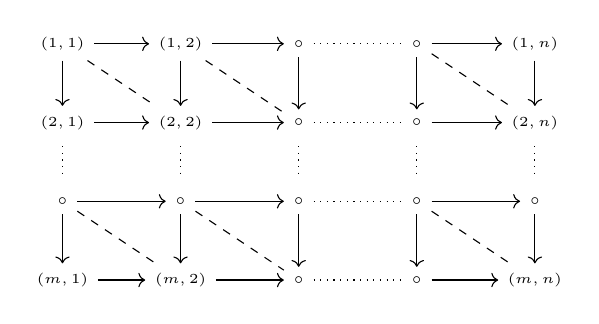
\begin{tikzpicture}
\node(11)at(0,0){\tiny{$(1,1)$}};
\node(12)at(1.5,0){\tiny{$(1,2)$}};
\node(13)at(3,0){\tiny{$\circ$}};
\draw[->](11)--(12);
\draw[->](12)--(13);
\node(14)at(4.5,0){\tiny{$\circ$}};
\node(15)at(6,0){\tiny{$(1,n)$}};
\draw[-,dotted](13)--(14);
\draw[->](14)--(15);
\node(21)at(0,-1){\tiny{$(2,1)$}};
\node(22)at(1.5,-1){\tiny{$(2,2)$}};
\node(23)at(3,-1){\tiny{$\circ$}};
\draw[->](21)--(22);
\draw[->](22)--(23);
\node(24)at(4.5,-1){\tiny{$\circ$}};
\node(25)at(6,-1){\tiny{$(2,n)$}};
\draw[-,dotted](23)--(24);
\draw[->](24)--(25);
\draw[->](15)--(25);
\draw[->](14)--(24);
\draw[->](13)--(23);
\draw[->](12)--(22);
\draw[->](11)--(21);
\draw[-,dashed](11)--(22);
\draw[-,dashed](12)--(23);
\draw[-,dashed](14)--(25);
\node(m1)at(0,-2){\tiny{$\circ$}};
\node(m2)at(1.5,-2){\tiny{$\circ$}};
\node(m3)at(3,-2){\tiny{$\circ$}};
\draw[->](m1)--(m2);
\draw[->](m2)--(m3);
\node(m4)at(4.5,-2){\tiny{$\circ$}};
\node(m5)at(6,-2){\tiny{$\circ$}};
\draw[-,dotted](m3)--(m4);
\draw[->](m4)--(m5);
\draw[-,dotted](6,-1.3)--(6,-1.7);
\draw[-,dotted](4.5,-1.3)--(4.5,-1.7);
\draw[-,dotted](3,-1.3)--(3,-1.7);
\draw[-,dotted](1.5,-1.3)--(1.5,-1.7);
\draw[-,dotted](0,-1.3)--(0,-1.7);
\node(n1)at(0,-3){\tiny{$(m,1)$}};
\node(n2)at(1.5,-3){\tiny{$(m,2)$}};
\node(n3)at(3,-3){\tiny{$\circ$}};
\draw[->](n1)--(n2);
\draw[->](n2)--(n3);
\node(n4)at(4.5,-3){\tiny{$\circ$}};
\node(n5)at(6,-3){\tiny{$(m,n)$}};
\draw[-,dotted](n3)--(n4);
\draw[->](n4)--(n5);
\draw[-,dashed](m1)--(n2);
\draw[-,dashed](m2)--(n3);
\draw[-,dashed](m4)--(n5);
\draw[->](m5)--(n5);
\draw[->](m4)--(n4);
\draw[->](m3)--(n3);
\draw[->](m2)--(n2);
\draw[->](m1)--(n1);
\end{tikzpicture}
\caption{the quiver which is a ``rectangle''}
\end{figure}
We introduce the gluing ``rectangles'' (see Definition \ref{defnOfGluing}) and investigate the derived equivalences between them. The main work of this paper is to establish the derived equivalence between all the Nakayama algebras $N(uv-a,v+1)$ and the corresponding ``rectangles'' missing an angle which is the quiver ${\vphantom{Q(m,n)}}\negmedspace{Q(m,n)}^{-a}$ obtained from $Q(u,v)$ by deleting vertices $\{(1,n-i+1)\}_{i\in \eta}$. Similarly, the bound quivers ${\vphantom{Q(m,n)}}^{-a}\negmedspace{Q(m,n)},\;{\vphantom{Q(m,n)}}_{-a}\negmedspace{Q(m,n)},\;{\vphantom{Q(m,n)}}\negmedspace{Q(m,n)}_{-a}$ are formed by deleting the vertex set $\{(1,i)\}_{i\in \eta}$, $\{(m,i)\}_{i\in \eta}$, $\{(m,n-i+1)\}_{i\in \eta}$ from quiver $ Q(m,n)$ respectively. We denote the algebra associated by the bound quiver $Q$ by $A(Q)$. Then the main theorem of this article is as following.

\begin{thm}\label{main}
\textup{(See Corollary \ref{main1} and Theorem \ref{main2})} We have the following derived equivalences:
\begin{align*}
\textup{D}^{b}(A[{\vphantom{Q(m,n)}}^{-a}\negmedspace{Q(m,n)}]) \simeq \textup{D}^{b}(A[\;{\vphantom{Q(m,n)}}\negmedspace{Q(m,n)}^{-a}]) &\simeq \textup{D}^{b}(A[{\vphantom{Q(m,n)}}_{-a}\negmedspace{Q(m,n)}])\simeq \textup{D}^{b}(A[\;{\vphantom{Q(m,n)}}\negmedspace{Q(m,n)}_{-a}])\\
&\simeq{\textup{D}^{b}( N(uv-a,v+1))}.
\end{align*}  
\end{thm}

The paper is organized as follows. In Section \ref{Sect2}, we recall some derived equivalences between upper triangular matrix algebras in \cite{Lad2011} and induce a new derived equivalence (see Corollary \ref{derOfTri3}). Furthermore, we describe the bound quivers $\tilde{Q},\widehat{Q}$ associated to these derived equivalent algebras. In Section \ref{Sect3}, we introduce the gluing ``rectangles'' and find a derived equivalence between different gluing ``rectangles''. As a Corollary, we prove a part of Theorem \ref{main}. In Section \ref{Sect4}, we investigate the gluing ``rectangles'' to the Nakayama algebras and provide the derived equivalence between the ``rectangle'' missing an angle and the corresponding Nakayama algebra which finish another part proof of Theorem \ref{main}.

\section{2}\label{Sect2}

\subsection{Algebras and quivers}

Throughout this paper, ${\bf k}$ is an algebraically closed field of characteristic zero and the algebras are considered as basic and connected finite dimensional ${\bf k}$-algebras. 

Let $\{e_i|i=1,2,\cdots,n\}$ be a complete set of primitive orthogonal idempotents of an algebra $A$. Then $A$ can be naturally regarded as a standard matrix algebra $A=(e_iAe_j)_{1\leq i,j\leq n}$ and any element $a\in A$ is naturally identified as the linear combination $a = \sum_{i,j=1}^n e_i a e_j$.

Let $Q=(Q_0,Q_1,I)$ be a quiver with the vertex set $Q_0$, the arrow set $Q_1$ and the admissible ideal $I$. By Gabriel's theorem, there exists unique finite connected quiver $Q_A=(Q_{A,0},Q_{A,1})$ and some admissible ideal $I$ such that $A\cong kQ_A/I$. We will call $A$ the algebra associated to the bound quiver $Q_A$ which means $(Q_{A,0},Q_{A,1},I)$. 

In our paper we focus on the bound quiver $Q=(Q_0,Q_1,I)$ with all commutative relations and no-cycles. It implies that there exists at most one path from $i$ to $j$ for each vertices $i,j\in Q_0$. We denote by $p_{i\to j}$ the only path from $i$ to $j$ if exists. Obviously, there is a natural partial order $\leq$ on $Q_0$: $i\leq j$ if and only if there is a path from $i$ to $j$ in $(Q_0,Q_1)$. Then the algebra associated to the bound quiver $Q$ can be an upper triangular matrix algebra, that is, $e_iAe_j=0$ for $i>j$. For simplicity, we will denote by $T(R,S;M)$ the upper triangular ring
$$\begin{pmatrix}
R  & M\\
0  & S
\end{pmatrix}.$$

\subsection{Derived equivalences between upper triangular matrix algebras}
In this subsection, we will recall some derived equivalences between triangular matrix algebras and show an unexpected derived equivalence as a corollary. 

First, Ladkani \cite{Lad2011} deduced a derived equivalence which will play a key role in our paper between triangular matrix algebras by constructing a tilting complex. 

\begin{prop} \textup{\cite[Theorem 4.5]{Lad2011}} \label{TiltingMod}
Let $R,S$ be rings and $T_S$ a tilting $S$-module. Let ${_R}M_S$ be an $R$-$S$-bimodule such that $M_S\in\textup{per}\;S$, that is $M_S$ is a right $S$-module and quasi-isomorphic to a bounded complex of finitely generated projective $S$-modules in $\textup{D}^{b}(S)$, and $\textup{Ext}^n_S(M_S,T_S)=0$ for all $n>0$.
Then the triangular matrix rings 
$$\begin{pmatrix}
R  & M\\
0  & S
\end{pmatrix}\,\,\,\,\,\,
and\,\,\,\,\,\,
\begin{pmatrix}
\textup{End}_{S}(T_S)  & \textup{Hom}{_S(M,T_S)}\\  
0  & R      
\end{pmatrix}$$are derived equivalent. 
\end{prop}

According to this Proposition, Ladkani also showed the following Corollary holds by taking $T_S=S$ and $T_S=\textup{D}(S)$ where $\textup{D}=\textup{Hom}_{\bf k} ({-}, {\bf k})$ is the standard duality.

\begin{cor} \textup{\cite[Corollary 4.9 and 4.11]{Lad2011}}
Let $R,S$ be algebras and ${_R}M_S$ an $R$-$S$-bimodule.
\begin{itemize}
    \item[(1)] If $M_S\in\textup{per}\;S$ and $\textup{Ext}^n_S(M_S,S)=0$ for all $n>0$. Then there is a derived equivalence between the triangular matrix algebras $T(R,S;M)$ and $T\big(S,R;\textup{Hom}{_S}(M,S)\big)$;
    \item[(2)] If $S$ is an Artin algebra with $\textup{gl.dim}\;S<\infty$ and $M$ is finitely generated as an $S$-module. Then there is a derived equivalence between $T(R,S;M)$ and $T(S,R;\textup{D}M)$.
\end{itemize}
\end{cor}

Our paper aims to study the ``gluing'' of ``rectangle'' algebras which is derived equivalent to the tensor product algebra of path algebras with type $\vec{A}$. For this purpose, we need the following Corollary as a byproduct of Proposition \ref{TiltingMod}. Our convention is that $\otimes$ (without subscript) will always mean tensor product over ${\bf k}$.

\begin{cor}\label{derOfTri3}
Let $R,S$ be algebras. Assume that $M$ is projective $S$-module and $N$ is projective ${\bf k}\vec{A}_n$-module. Then there exists a derived equivalence between the triangular matrix algebras $T(R\otimes{\bf k}\vec{A}_m,S\otimes{\bf k}\vec{A}_n;M\otimes N)$ and $T\big(S\otimes{\bf k}\vec{A}_n,R\otimes{\bf k}\vec{A}_m;\textup{Hom}_{S}(M,S)\otimes\textup{D}(N)\big)$.    
\end{cor}

\begin{proof}
Let $T=S\otimes_{\bf k}\textup{D}({\bf k}\vec{A}_n)$. Since $S$ is a tilting $S$-module and $\textup{D}({\bf k} \vec{A}_n)$ is a tilting ${\bf k}\vec{A}_n$-module, $T$ is a tilting $S\otimes {\bf k}\vec{A}_n$-module by \cite[Theorem A]{Lad2012} {\color{red}whose endomorphism algebra is isomorphic to $S\otimes{\bf k}\vec{A}_n$.}{\color{blue}Need prove!}

Moreover $M$ is projective as $S$-module and $N$ is projective as ${\bf k}\vec{A}_n$-module. By \cite[Lemma 2.1]{Lad2012}, we have
\begin{equation}\label{2111}
\textup{Hom}_{S\otimes{\bf k}\vec{A}_n}(M\otimes N,T)=\textup{Hom}_{S}(M,S)\otimes\textup{Hom}_{{\bf k}\vec{A}_n}(N,\textup{D}({\bf k} \vec{A}_n))
\end{equation}

According to the Hom-tensor adjointness, We have
\begin{align}
\textup{Hom}_{{\bf k}\vec{A}_n}(N,\textup{D}({\bf k} \vec{A}_n))&=\textup{Hom}_{{\bf k}\vec{A}_n}\big(N,\textup{Hom}_{\bf k}({\bf k} \vec{A}_n,{\bf k})\big)\notag\\
&=\textup{Hom}_{\bf k}(N\otimes_{{\bf k}\vec{A}_n}{\bf k}\vec{A}_n,{\bf k})=\textup{D}(N)\label{2112}
\end{align}
Combine formulas (\ref{2111}) and (\ref{2112}), it follows that $\textup{Hom}_{S\otimes{\bf k}\vec{A}_n}(M\otimes N,T)=\textup{Hom}_{S}(M,S)\otimes\textup{D}(N)$. Hence the result holds by Proposition \ref{TiltingMod}.
\end{proof}

\subsection{Shadow}
Let $Q=(Q_0,Q_1,I)$ be a quiver with all commutative relations and no-cycles. Now we define the shadow of a vertex.
\begin{defn}
For a vertex $i\in Q_0$ and a subset $T\subseteq Q_0$, we say $j$ is the \emph{shadow} of $i$ in $T$ if there exists the unique vertex $j$ in $T$ such that each path $p_{i\to t}$ ($t\in T$) can factor through non-zero $p_{i\to j}$.
\end{defn}

Let $\Omega(i,T)=\{t\in T|\textup{there exists a path from}\;i\;\textup{to}\;t\;\textup{in}\;Q\}$. The next lemma gives a description of the shadow.
\begin{lem}
For a subset $T\subseteq Q_0$, let $i$ be the vertex such that $\Omega(i,T)$ is non-empty. Then $j$ is the shadow of $i$ in $T$ if and only if $j$ is the minimum element in $\Omega(i,T)$.
\end{lem}

\begin{proof}
For any $t\in\Omega(i,T)$, there exists a path $p_{i\to t}$ in $Q$. If $j$ is the shadow of $i$ in $T$, we have $p_{i\to t}=p_{i\to j}p_{j\to t}$. Then there exists a path from $j$ to $t$ in $(Q_0,Q_1)$, that is, $j\leq t$. Hence $j$ is the minimum element in $\Omega(i,T)$.

Conversely, assume that there exists the minimum element $j$ in $\Omega(i,T)$. Then $j\leq t$ for any $t\in\Omega(i,T)$ by the minimum property of $j$. It implies $p_{i\to t}=p_{i\to j}p_{j\to t}$ in $(Q_0,Q_1)$, which also holds in $Q$ when $p_{i\to t}$ is non-zero. That is, each non-zero $p_{i\to t}$ can factor through non-zero $p_{i\to j}$. Hence $j$ is the shadow of $i$ in $T$.
\end{proof}

Let $Q$ be a quiver. Assume that $T\subseteq Q_0$ satisfies that $\Omega(i,T)$ has the minimum element for each vertex $i$ with non-empty set $\Omega(i,T)$. We define a map $f_T$ on $Q_0$ as following:
\begin{align*}
(1)\;f_T(i)\;\textup{is the shadow of}\;i\;\textup{in}\;T\;\textup{when}\;\Omega(i,T)\neq\emptyset;\;\;\;\;\;\;&(2)\;f_T(i)=i\;\textup{when}\;\Omega(i,T)=\emptyset.
\end{align*}

\subsection{Derived equivalence between bound quiver algebras}
Let $Q=(Q_0,Q_1,I)$ be a quiver with all commutative relations and no-cycles, that is, the associated algebra $A={\bf k}Q/I$ is an upper triangular ring $T(R,S;M)$. We may assume that $Q_0=Q_{R,0}\cup Q_{S,0}$.

In this subsection, we always assume that each non-empty set $\Omega(i,Q_{S,0})$ has the minimum element for each vertex $i\in Q_0$. Our main result is to construct two quivers $\tilde{Q},\widehat{Q}$ whose associated algebras are both derived equivalent to $A$. Because the proof of Proposition \ref{210} and \ref{211} are long and tedious, we put them in the next single subsection.

Let $f_S$ be the map $f_{Q_{S,0}}$, and denote by $f_S^{*}(j)$ the set $\{i\in Q_{R,0}|f_S(i)=j\}$ for each $j\in Q_{S,0}$.

\begin{defn}\label{Def210}
For the bound quiver $Q$ of the algebra $A$, we construct $\tilde{Q}=(\tilde{Q}_0,\tilde{Q}_1,\tilde{I})$ as following.
\begin{itemize}
    \item $\tilde{Q}_0=Q_0=Q_{R,0}\cup Q_{S,0}$;
    \item $\tilde{Q}$ contains all arrows which are in $Q_R$ or $Q_S$;
    %for arrow $\alpha:\;i\rightarrow j$ in $Q$ with $i,j\in Q_{R,0}$ (or $i,j\in Q_{S,0}$), then $\tilde{Q}$ also contains $\alpha$;
    \item adding the arrow $\alpha_{ji} : j \to i $ whenever $j\in Q_{S,0}$ and $i$ is a minimal element in $f_S^{*}(j)$; 
    \item $\tilde{I}$ contains all relations in $I$ whenever the corresponding paths are in $(\tilde{Q}_0,\tilde{Q}_1)$;
    \item adding zero relation $\alpha_{ji}\circ p_{i\to f_S(i')}$ whenever $p_{j\to i'}=0$ for $i' \in Q_{R,0}$, and zero relation $p_{j'\to j}\circ\alpha_{ji}$ whenever $p_{j'\to f_S(i)}=0$ for $j'\in Q_{S,0}${\color{red}[this part always holds?]}; 
    \item adding the commutative relations from $j\in Q_{S,0}$ to $i\in Q_{R,0}$ if there exist more than one path from $j$ to $i$.
\end{itemize}
\end{defn}

\begin{prop} \label{210}
We have $\textup{D}^b\big({\bf k} Q/I\big)\simeq \textup{D}^b\big({\bf k} \tilde{Q}/\tilde{I}\big)$. 
\end{prop}

Let $\Gamma(R) = \{i\in Q_{R,0}|p_{i\to j}\neq 0, \textup{there exists}\;j\in Q_{S,0}\}$ and $\Gamma(S) = \{j\in Q_{R,0}|p_{i\to j}\neq 0, \textup{there exists}\;i\in Q_{R,0}\}$. Denote by $m(R)\;\big(\textup{resp.}\;M(S)\big)$ the set of the minimal vertices in $R$ (resp. the maximal vertices in $S$). If there exists non-zero path from $i$ to $j$ in $Q$ for all $i\in m(R)$ and $j\in M(S)$, we construct $\widehat{Q}$ as following.

\begin{defn}\label{Def211}
For the bound quiver $Q$ of the algebra $A$, we construct $\widehat{Q}=(\widehat{Q}_0,\widehat{Q}_1,\widehat{I})$ as following.
\begin{itemize}
    \item $\widehat{Q}_0=Q_0=Q_{R,0}\cup Q_{S,0}$;
    \item $\widehat{Q}$ contains all arrows which are in $Q_R$ or $Q_S$;
    %for arrow $\alpha:\;i\rightarrow j$ in $Q$ with $i,j\in Q_{R,0}$ (or $i,j\in Q_{S,0}$), then $\tilde{Q}$ also contains $\alpha$;
    \item adding the arrow $\beta_{ji} : j\to i$ whenever $j\in M(S)$ and $i\in m(R)$;
    \item $\tilde{I}$ contains all relations in $I$ whenever the corresponding paths are in $(\tilde{Q}_0,\tilde{Q}_1)$;
    \item {\color{blue}adding zero relation $p_{j'j}\circ \beta_{ji}\circ p_{ii'}$ where $j\in M(S)$ and $i\in m(R)$ whenever $p_{j'\to i'}=0$ in $Q$;}
    \item adding commutative relations from $j\in Q_{S,0}$ to $i\in Q_{R,0}$ if there exist more than one path from $j$ to $i$ in $Q$.
\end{itemize}
\end{defn}

\begin{prop}\label{211}
If  $\textup{gl.dim}\;S<\infty$, then we have  $\textup{D}^b\big({\bf k} Q/I\big)\simeq \textup{D}^b\big({\bf k} \widehat{Q}/\widehat{I}\big)$.  
\end{prop}

\subsection{Proof of Proposition \ref{210} and \ref{211}}

\section{}\label{Sect3}

In this section, we will apply the construction in Definition \ref{Def210} and \ref{Def211} and use Proposition \ref{210} and \ref{211} to get some derived equivalences between ``rectangles'' under the different gluing methods.

\subsection{Gluing ``rectangles''}
\begin{defn}\label{defnOfGluing}
Let $r$ be a positive integer. Denote by $\mathscr{L}=\{{\bf{l}}_{ij}|1\leq i\neq j\leq r\}$ the set of vectors, where the dimension of ${\bf{l}}_{ij}$ and ${\bf{l}}_{ji}$ are equal. Denote by ${\bf{l}}_{ij}=(l_{ij}^{(k)})$ where $l_{ij}^{(k)}$ is an integer with $1\leq l_{ij}^{(k)}<l_{ij}^{(k+1)}\leq m_i$. Take ${\bf{l}}_i=\{{\bf{l}}_{ij}|j\neq i\}$. We define by $\#_{i=1}^r Q(m_i,n_i;{\bf{l}}_i)=Q(m_1,n_1;{\bf{l}}_1)\#Q(m_2,n_2;{\bf{l}}_2)\#\cdots\#Q(m_r,n_r;{\bf{l}}_r)$ the quiver by gluing quivers $Q(m_i,n_i)\;(1\leq i\leq r)$ as following:
\begin{itemize}
\item the vertex set is $\bigcup_{i=1}^r  Q(m_i,n_i)$; and in order to distinguish the vertex in different rectangles, we will use $(a,b;i)$ to represent the vertex $(a,b)$ in $Q(m_i,n_i)$;
\item we reserve the arrows in all rectangles, and add the arrow from $(l_{ij}^{(k)},n_i;i)$ to $(l_{ji}^{(k)},1;j)$ for each $1\leq i<j\leq r$;
\item we reserve the relations in all rectangles, and add the relations which makes the paths from $(l_{ij}^{(k)},n_i;i)$ to $(l_{ji}^{(k')},1;j)$ commute for each $1\leq i<j\leq r$ and $k\leq k'$.
\end{itemize}
\end{defn}

\begin{exm}\label{ExamOfGluing}
\begin{itemize}
    \item[(1)] If $r=2$ and the dimension of ${\bf{l}}_{12},{\bf{l}}_{21}$ are both $k$, the bound quiver $Q(m_1,n_1;{\bf{l}}_{12})$\# $Q(m_2,n_2;{\bf{l}}_{21})$ is the quiver as following with all commutative relations.
\begin{figure}[H]\centering
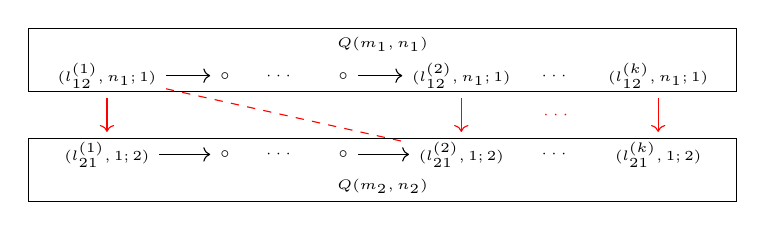
\begin{tikzpicture}
\draw[-](-1,1.6)--(8,1.6);
\draw[-](-1,0.8)--(8,0.8);
\draw[-](8,0.8)--(8,1.6);
\draw[-](-1,0.8)--(-1,1.6);
\node()at(3.5,1.4){\tiny{$Q(m_1,n_1)$}};
\draw[-](-1,0.2)--(8,0.2);
\draw[-](-1,-0.6)--(8,-0.6);
\draw[-](8,-0.6)--(8,0.2);
\draw[-](-1,-0.6)--(-1,0.2);
\node()at(3.5,-0.4){\tiny{$Q(m_2,n_2)$}};
\node(m5)at(0,1){\tiny{$(l_{12}^{(1)},n_1;1)$}};
\node(m4)at(1.5,1){\tiny{$\circ$}};
\node()at(2.2,1){\tiny{$\cdots$}};
\node(m3)at(3,1){\tiny{$\circ$}};
\node(m2)at(4.5,1){\tiny{$(l_{12}^{(2)},n_1;1)$}};
\node()at(5.7,1){\tiny{$\cdots$}};
\draw[->](m5)--(m4);
\draw[->](m3)--(m2);
\node(m1)at(7,1){\tiny{$(l_{12}^{(k)},n_1;1)$}};
\node(n5)at(0,0){\tiny{$(l_{21}^{(1)},1;2)$}};
\node(n4)at(1.5,0){\tiny{$\circ$}};
\node()at(2.2,0){\tiny{$\cdots$}};
\node(n3)at(3,0){\tiny{$\circ$}};
\node(n2)at(4.5,0){\tiny{$(l_{21}^{(2)},1;2)$}};
\draw[->](n5)--(n4);
\draw[->](n3)--(n2);
\draw[->,red](m5)--(n5);
\draw[->,red](m2)--(n2);
\draw[-,dashed,red](m5)--(n2);
\node()at(5.7,0){\tiny{$\cdots$}};
\node()at(5.7,0.5){\tiny{${\color{red}\cdots}$}};
\node(n1)at(7,0){\tiny{$(l_{21}^{(k)},1;2)$}};
\draw[->,red](m1)--(n1);
\end{tikzpicture}
\caption{the quiver $Q(m_1,n_1;{\bf{l}}_{12})\#Q(m_2,n_2;{\bf{l}}_{21})$}
\end{figure}
\item[(2)] If $r=3$ and $m_1=m_3$, we take ${\bf{l}}_{13}={\bf{l}}_{31}=\{1,2,3,\cdots,m_1\}$, ${\bf{l}}_{21}={\bf{l}}_{23}=\{1,2,3,\cdots,m_2\}$, ${\bf{l}}_{12}={\bf{l}}_{32}=\{l_1,l_2,l_3,\cdots,l_{m_2}\}$. The bound quiver $Q(m_1,n_1;{\bf{l}}_{12},{\bf{l}}_{13})$\#$Q(m_2,n_2;{\bf{l}}_{21},{\bf{l}}_{23})$\# $Q(m_3,n_3;{\bf{l}}_{31},{\bf{l}}_{32})$ is the quiver as following with all commutative relations.

\begin{figure}[H]
\tiny{
\begin{tikzcd}
	{\small\bullet} & \small\bullet & \small\bullet & {\small(1,n_1;1)} &&&&& {\small(1,1;3)} & \small\bullet & \small\bullet & {\small\bullet} \\
	\small\bullet & \small\bullet & \small\bullet & \small\bullet &&&&& \small\bullet & \small\bullet & \small\bullet & \small\bullet \\
	\small\bullet & \small\bullet & \small\bullet & {\small(l_1,n_1;1)} & {\small(1,1;2)} & \small\bullet & \small\bullet & {\small(1,n_2;2)} & {\small(l_{1},1;3)} & \small\bullet & \small\bullet & \small\bullet \\
	\small\bullet & \small\bullet & \small\bullet & \small\bullet & {} & { } & {} & {} & \small\bullet & \small\bullet & \small\bullet & \small\bullet \\
	\small\bullet & \small\bullet & \small\bullet & \small\bullet & {} & {} & {} & {} & \small\bullet & \small\bullet & \small\bullet & \small\bullet \\
	\small\bullet & \small\bullet & \small\bullet & {\small(l_2,n_1;1)} & {\small(2,1;2)} & \small\bullet & \small\bullet & \small\bullet & {\small(l_{2},1;3)} & \small\bullet & \small\bullet & \small\bullet \\
	\small\bullet & \small\bullet & \small\bullet & \small\bullet & \small\bullet & \small\bullet & \small\bullet & \small\bullet & \small\bullet & \small\bullet & \small\bullet & \small\bullet \\
	\small\bullet & \small\bullet & \small\bullet & \small\bullet & {} & {} & {} & {} & \small\bullet & \small\bullet & \small\bullet & \small\bullet \\
	\small\bullet & \small\bullet & \small\bullet & \small\bullet & {} & {} & {} & {} & \small\bullet & \small\bullet & \small\bullet & \small\bullet \\
	\small\bullet & \small\bullet & \small\bullet & {\small(l_{m_2},n_1;1)} & {\small(m_2,1;2)} & \small\bullet & \small\bullet & {\small(m_2,n_2;2)} & {\small(l_{m_2},1;3)} & \small\bullet & \small\bullet & \small\bullet \\
	\small\bullet & \small\bullet & \small\bullet & \small\bullet &&&&& \small\bullet & \small\bullet & \small\bullet & \small\bullet \\
	\small\bullet & \small\bullet & \small\bullet & {\small(m_1,n_1;1)} &&&&& {\small(m_3,1;3)} & \small\bullet & \small\bullet & \small\bullet
	\arrow[from=7-6, to=10-6]
	\arrow[from=10-5, to=10-6]
	\arrow[from=7-5, to=7-6]
	\arrow[from=7-5, to=10-5]
	\arrow[from=3-5, to=6-5]
	\arrow[from=10-7, to=10-8]
	\arrow[from=7-7, to=10-7]
	\arrow[from=7-7, to=7-8]
	\arrow[from=7-8, to=10-8]
	\arrow[from=6-7, to=6-8]
	\arrow[from=3-7, to=6-7]
	\arrow[from=3-7, to=3-8]
	\arrow[from=3-8, to=6-8]
	\arrow[dotted, no head, from=6-5, to=7-5]
	\arrow[dotted, no head, from=7-6, to=7-7]
	\arrow[dotted, no head, from=10-6, to=10-7]
	\arrow[dotted, no head, from=6-8, to=7-8]
	\arrow[dotted, no head, from=6-7, to=7-7]
	\arrow[from=2-3, to=2-4]
	\arrow[dotted, no head, from=1-2, to=1-3]
	\arrow[from=1-3, to=1-4]
	\arrow[from=1-3, to=2-3]
	\arrow[from=1-4, to=2-4]
	\arrow[from=1-1, to=1-2]
	\arrow[from=1-1, to=2-1]
	\arrow[from=2-1, to=2-2]
	\arrow[from=1-2, to=2-2]
	\arrow[dotted, no head, from=2-2, to=2-3]
	\arrow[from=11-4, to=12-4]
	\arrow[from=11-3, to=11-4]
	\arrow[from=11-3, to=12-3]
	\arrow[from=12-3, to=12-4]
	\arrow[dotted, no head, from=11-2, to=11-3]
	\arrow[from=11-2, to=12-2]
	\arrow[dotted, no head, from=12-2, to=12-3]
	\arrow[from=11-1, to=11-2]
	\arrow[from=11-1, to=12-1]
	\arrow[from=12-1, to=12-2]
	\arrow[dotted, no head, from=2-1, to=3-1]
	\arrow[from=3-1, to=3-2]
	\arrow[dotted, no head, from=2-2, to=3-2]
	\arrow[dotted, no head, from=2-3, to=3-3]
	\arrow[from=3-3, to=3-4]
	\arrow[dotted, no head, from=2-4, to=3-4]
	\arrow[from=3-3, to=4-3]
	\arrow[from=4-3, to=4-4]
	\arrow[from=3-4, to=4-4]
	\arrow[from=3-2, to=4-2]
	\arrow[from=3-1, to=4-1]
	\arrow[from=4-1, to=4-2]
	\arrow[from=5-3, to=5-4]
	\arrow[from=5-4, to=6-4]
	\arrow[from=5-3, to=6-3]
	\arrow[from=6-3, to=6-4]
	\arrow[from=5-1, to=6-1]
	\arrow[from=5-1, to=5-2]
	\arrow[from=6-1, to=6-2]
	\arrow[from=7-3, to=7-4]
	\arrow[from=7-4, to=8-4]
	\arrow[from=7-3, to=8-3]
	\arrow[from=8-3, to=8-4]
	\arrow[from=7-1, to=7-2]
	\arrow[from=7-2, to=8-2]
	\arrow[from=7-1, to=8-1]
	\arrow[from=8-1, to=8-2]
	\arrow[from=9-3, to=9-4]
	\arrow[from=9-4, to=10-4]
	\arrow[from=9-3, to=10-3]
	\arrow[from=10-3, to=10-4]
	\arrow[from=9-1, to=9-2]
	\arrow[from=9-2, to=10-2]
	\arrow[from=9-1, to=10-1]
	\arrow[from=10-1, to=10-2]
	\arrow[dotted, no head, from=10-3, to=11-3]
	\arrow[dotted, no head, from=10-4, to=11-4]
	\arrow[dotted, no head, from=10-2, to=11-2]
	\arrow[dotted, no head, from=10-1, to=11-1]
	\arrow[dotted, no head, from=10-2, to=10-3]
	\arrow[dotted, no head, from=9-2, to=9-3]
	\arrow[dotted, no head, from=8-2, to=8-3]
	\arrow[dotted, no head, from=7-2, to=7-3]
	\arrow[from=5-2, to=6-2]
	\arrow[dotted, no head, from=5-2, to=5-3]
	\arrow[dotted, no head, from=6-2, to=6-3]
	\arrow[dotted, no head, from=4-2, to=4-3]
	\arrow[dotted, no head, from=3-2, to=3-3]
	\arrow[dotted, no head, from=4-1, to=5-1]
	\arrow[dotted, no head, from=4-2, to=5-2]
	\arrow[dotted, no head, from=4-3, to=5-3]
	\arrow[dotted, no head, from=6-1, to=7-1]
	\arrow[dotted, no head, from=6-2, to=7-2]
	\arrow[dotted, no head, from=6-3, to=7-3]
	\arrow[dotted, no head, from=6-4, to=7-4]
	\arrow[dotted, no head, from=8-1, to=9-1]
	\arrow[dotted, no head, from=8-2, to=9-2]
	\arrow[dotted, no head, from=8-3, to=9-3]
	\arrow[dotted, no head, from=8-4, to=9-4]
	\arrow[from=6-5, to=6-6]
	\arrow[dotted, no head, from=6-6, to=7-6]
	\arrow[dotted, no head, from=6-6, to=6-7]
	\arrow[from=3-6, to=6-6]
	\arrow[from=3-5, to=3-6]
	\arrow[dotted, no head, from=3-6, to=3-7]
	\arrow[from=2-9, to=2-10]
	\arrow[from=1-9, to=1-10]
	\arrow[from=1-11, to=1-12]
	\arrow[from=2-11, to=2-12]
	\arrow[dotted, no head, from=2-9, to=3-9]
	\arrow[from=3-9, to=3-10]
	\arrow[dotted, no head, from=2-10, to=3-10]
	\arrow[dotted, no head, from=2-11, to=3-11]
	\arrow[from=3-11, to=3-12]
	\arrow[dotted, no head, from=2-12, to=3-12]
	\arrow[from=3-9, to=4-9]
	\arrow[from=4-9, to=4-10]
	\arrow[from=3-10, to=4-10]
	\arrow[from=3-11, to=4-11]
	\arrow[from=4-11, to=4-12]
	\arrow[from=3-12, to=4-12]
	\arrow[from=5-9, to=6-9]
	\arrow[from=5-9, to=5-10]
	\arrow[from=5-10, to=6-10]
	\arrow[from=6-9, to=6-10]
	\arrow[from=5-11, to=5-12]
	\arrow[from=5-11, to=6-11]
	\arrow[from=6-11, to=6-12]
	\arrow[from=5-12, to=6-12]
	\arrow[from=7-9, to=7-10]
	\arrow[from=7-9, to=8-9]
	\arrow[from=7-10, to=8-10]
	\arrow[from=8-9, to=8-10]
	\arrow[from=7-11, to=7-12]
	\arrow[from=7-12, to=8-12]
	\arrow[from=7-11, to=8-11]
	\arrow[from=8-11, to=8-12]
	\arrow[from=9-9, to=10-9]
	\arrow[from=9-9, to=9-10]
	\arrow[from=9-10, to=10-10]
	\arrow[from=9-11, to=9-12]
	\arrow[from=9-12, to=10-12]
	\arrow[from=9-11, to=10-11]
	\arrow[from=10-9, to=10-10]
	\arrow[from=10-11, to=10-12]
	\arrow[dotted, no head, from=10-9, to=11-9]
	\arrow[from=11-9, to=11-10]
	\arrow[dotted, no head, from=10-10, to=11-10]
	\arrow[dotted, no head, from=10-11, to=11-11]
	\arrow[from=11-11, to=11-12]
	\arrow[dotted, no head, from=10-12, to=11-12]
	\arrow[from=12-9, to=12-10]
	\arrow[from=12-11, to=12-12]
	\arrow[dotted, no head, from=1-10, to=1-11]
	\arrow[dotted, no head, from=2-10, to=2-11]
	\arrow[dotted, no head, from=3-10, to=3-11]
	\arrow[dotted, no head, from=4-10, to=4-11]
	\arrow[dotted, no head, from=5-10, to=5-11]
	\arrow[dotted, no head, from=6-10, to=6-11]
	\arrow[dotted, no head, from=7-10, to=7-11]
	\arrow[dotted, no head, from=8-10, to=8-11]
	\arrow[dotted, no head, from=9-10, to=9-11]
	\arrow[dotted, no head, from=10-10, to=10-11]
	\arrow[dotted, no head, from=11-10, to=11-11]
	\arrow[dotted, no head, from=12-10, to=12-11]
	\arrow[from=1-9, to=2-9]
	\arrow[from=1-10, to=2-10]
	\arrow[from=1-11, to=2-11]
	\arrow[from=1-12, to=2-12]
	\arrow[dotted, no head, from=4-9, to=5-9]
	\arrow[dotted, no head, from=4-10, to=5-10]
	\arrow[dotted, no head, from=4-11, to=5-11]
	\arrow[dotted, no head, from=4-12, to=5-12]
	\arrow[dotted, no head, from=6-9, to=7-9]
	\arrow[dotted, no head, from=6-10, to=7-10]
	\arrow[dotted, no head, from=6-11, to=7-11]
	\arrow[dotted, no head, from=6-12, to=7-12]
	\arrow[dotted, no head, from=8-9, to=9-9]
	\arrow[dotted, no head, from=8-10, to=9-10]
	\arrow[dotted, no head, from=8-11, to=9-11]
	\arrow[dotted, no head, from=8-12, to=9-12]
	\arrow[from=11-9, to=12-9]
	\arrow[from=11-10, to=12-10]
	\arrow[from=11-11, to=12-11]
	\arrow[from=11-12, to=12-12]
	\arrow[color={rgb,255:red,255;green,58;blue,51}, from=3-4, to=3-5]
	\arrow[color={rgb,255:red,255;green,58;blue,51}, from=6-4, to=6-5]
	\arrow[color={rgb,255:red,255;green,58;blue,51}, from=7-4, to=7-5]
	\arrow[color={rgb,255:red,255;green,58;blue,51}, from=10-4, to=10-5]
	\arrow[color={rgb,255:red,255;green,58;blue,51}, from=3-8, to=3-9]
	\arrow[color={rgb,255:red,255;green,58;blue,51}, from=6-8, to=6-9]
	\arrow[color={rgb,255:red,255;green,58;blue,51}, from=10-8, to=10-9]
	\arrow[color={rgb,255:red,255;green,58;blue,51}, from=7-8, to=7-9]
	\arrow[from=1-4, to=1-9]
	\arrow[from=2-4, to=2-9]
	\arrow[from=11-4, to=11-9]
	\arrow[from=12-4, to=12-9]
	\arrow[no head, from=4-4, to=4-5]
	\arrow[no head, from=8-4, to=8-5]
	\arrow[no head, from=9-4, to=9-5]
	\arrow[no head, from=8-5, to=8-6]
	\arrow[no head, from=5-4, to=5-5]
	\arrow[no head, from=4-5, to=4-6]
	\arrow[no head, from=5-5, to=5-6]
	\arrow[no head, from=9-5, to=9-6]
	\arrow[no head, from=4-6, to=4-7]
	\arrow[no head, from=5-6, to=5-7]
	\arrow[no head, from=8-6, to=8-7]
	\arrow[no head, from=9-6, to=9-7]
	\arrow[no head, from=8-7, to=8-8]
	\arrow[no head, from=5-7, to=5-8]
	\arrow[no head, from=4-7, to=4-8]
	\arrow[no head, from=9-7, to=9-8]
	\arrow[from=4-8, to=4-9]
	\arrow[from=5-8, to=5-9]
	\arrow[from=8-8, to=8-9]
	\arrow[from=9-8, to=9-9]
	\arrow[dotted, no head, from=4-4, to=5-4]
\end{tikzcd}}
\caption{the quiver $Q(m_1,n_1;{\bf{l}}_{12},{\bf{l}}_{13})\#Q(m_2,n_2;{\bf{l}}_{21},{\bf{l}}_{23})\#Q(m_3,n_3;{\bf{l}}_{31},{\bf{l}}_{32})$}
\end{figure}
\end{itemize}
\end{exm}

\subsection{A derived equivalence on gluing ``rectangles''}
In this subsection, we focus on the gluing ``rectangles'' in Example \ref{ExamOfGluing}. For simplicity, we assume that $m_1\geq m_2$ and denote by $A_0$ the algebra associated to $Q(m_1,n_1;{\bf{l}}_{12})\#Q(m_2,n_2;{\bf{l}}_{21})$ where ${\bf{l}}_{21}=\{1,2,3,\cdots,m_2\}$ and ${\bf{l}}_{12}=\{l_1,l_2,l_3,\cdots,l_{m_2}\}$. Also we denote by $A_s$ the algebra associated to $Q(m_1,n_1-s;{\bf{l}}_{12},{\bf{l}}_{13})\#Q(m_2,n_2;{\bf{l}}_{21},{\bf{l}}_{23})\#Q(m_1,s;{\bf{l}}_{31},{\bf{l}}_{32})$ as in Example \ref{ExamOfGluing}(2) for $1\leq s\leq n_1$. The following derived equivalences are important.

\begin{prop}\label{As=At}
There exist the derived equivalences $\textup{D}^{b}(A_s) \simeq \textup{D}^{b}(A_t)$ for each $0\leq s,t\leq n$.   
\end{prop}

\begin{proof}
\end{proof}

\begin{exm}
\end{exm}

An immediate consequence of Proposition \ref{As=At} is as following.

\begin{cor}\label{main1}
Let $\eta = \{1,2,\dots,a\}$ for $1\leq a<n$. We have the following derived equivalences
$$
    \textup{D}^{b}(A[{\vphantom{Q(m,n)}}^{-a}\negmedspace{Q(m,n)}]) \simeq \textup{D}^{b}(A[\;{\vphantom{Q(m,n)}}\negmedspace{Q(m,n)}^{-a}]) \simeq \textup{D}^{b}(A[{\vphantom{Q(m,n)}}_{-a}\negmedspace{Q(m,n)}])\simeq \textup{D}^{b}(A[\;{\vphantom{Q(m,n)}}\negmedspace{Q(m,n)}_{-a}]).
    $$
\end{cor}

\begin{proof}
Denote by ${\bf{l}}=\{1,2,\cdots,n-a\}$. By Proposition \ref{As=At}, we have \begin{align*}
    \textup{D}^{b}(A[\;{\vphantom{Q(m,n)}}\negmedspace{Q(m,n)}_{-a}])&\simeq \textup{D}^{b}(A[Q(n,m-1;{\bf{l}})\#Q(n-a,1;{\bf{l}})])\\
    &\simeq\textup{D}^{b}(A[Q(n-a,1;{\bf{l}})\#Q(n,m-1;{\bf{l}})])\\
    &\simeq \textup{D}^{b}(A[\;{\vphantom{Q(m,n)}}\negmedspace{Q(m,n)}^{-a}]).
\end{align*}
Similarly, we have $\textup{D}^{b}(A[{\vphantom{Q(m,n)}}^{-a}\negmedspace{Q(m,n)}]) \simeq \textup{D}^{b}(A[{\vphantom{Q(m,n)}}_{-a}\negmedspace{Q(m,n)}])$. 

Moreover, denote by ${\bf{l}'}=\{1,2,\cdots,m-1\}$. By Proposition \ref{As=At}, we have \begin{align*}
    \textup{D}^{b}(A[\;{\vphantom{Q(m,n)}}\negmedspace{Q(m,n)}_{-a}])&\simeq \textup{D}^{b}(A[Q(m,n-a;{\bf{l}'})\#Q(m-1,a;{\bf{l}'})])\\
    &\simeq\textup{D}^{b}(A[Q(m-1,a;{\bf{l}'})\#Q(m,n-a;{\bf{l}'})])\\
    &\simeq \textup{D}^{b}(A[{\vphantom{Q(m,n)}}_{-a}\negmedspace{Q(m,n)}]).
\end{align*}
Hence we finish the proof.
\end{proof}



\section{The derived equivalences for studying the Nakayama algebras}\label{Sect4}

\subsection{Gluing with the Nakayama algebra}
The Nakayama algebra $N(n,r)$ is the bound quiver algebra of the equioriented quiver
$$\xymatrix{1\ar[r]^{x}&2\ar[r]^{x}&3\ar[r]^{x}&\cdots\ar[r]^{x}&n-1\ar[r]^{x}&n}$$
of type $\vec{A}_n$ subject to all relations $x^r=0$. Clearly, we may regard $Q_{N(n,r)}$ as the quiver $\vec{A}_n$ with admissible ideal $(x^r)$. For convenience, we denote $Q^{(r)}(n,1)=Q_{N(n,r)}$. Similar to Definition \ref{defnOfGluing}, we can define by $Q(u,v;{\bf l}_0)\#Q^{(r)}(n,1;{\bf l})$ the quiver $Q(u,v;{\bf l}_0)\#Q(n,1;{\bf l})$ preserving the relations in $Q_{N(n,r)}$ for $u\leq r$, where ${\bf l}_0=\{1,2,\cdots,u\}$ and ${\bf l}=\{l_1,l_2,\cdots,l_u\}$. We have the following proposition.

\begin{prop}\label{Rect+Naka}
Let $u\leq r$. Take ${\bf l}_0=\{1,2,\cdots,u\}$, ${\bf l}=\{l_1,l_2,\cdots,l_u\}$, then we have the following derived equivalences
\begin{itemize}
    \item[(1)] $\textup{D}^{b}\big(A[Q(u,v;{\bf l}_0)\#Q^{(r)}(n,1;{\bf l})]\big)\simeq\textup{D}^{b}\big(A[Q^{(r)}(n,1;{\bf l})\#Q(u,v;{\bf l}_0)]\big).$
    \item[(2)] $\textup{D}^{b}\big(A[Q(u,v;{\bf l}_0)\#Q^{(u+1)}(n,1;{\bf l}_0)\big)\simeq\textup{D}^{b}\big(A[Q(u,v-1;{\bf l}_0)\#Q^{(u+1)}(n+u,1;{\bf l}_0)]\big)$
\end{itemize}
\end{prop}

\begin{proof}
    
\end{proof}

\begin{exm}
    
\end{exm}

\subsection{}
For the purpose of studying the Nakayama algebras, we need the significant proposition \ref{derivedImp} which establishes the derived equivalence between a Nakayama algebra and gluing ``rectangles''.

\begin{prop}\label{derivedImp}
Let ${\bf l}=\{1,2,\cdots,u\}$ and $x$ be an integer greater than or equal to $2$. Then there exists the derived equivalence
$$\textup{D}^{b}(A[Q(u,v-1;{\bf{l}})\#Q^{(u+1)}(u+x,1;{\bf{l}})])\simeq\textup{D}^{b}(N(uv+x,u+1)).$$
\end{prop}

\begin{proof}
By induction and using Proposition \ref{Rect+Naka}(2), we have
\begin{align*}
    \textup{D}^{b}(A[Q(u,v-1;{\bf{l}})\#Q^{(u+1)}(u+x,1;{\bf{l}})])&\simeq \textup{D}^{b}(A[Q(u,v-2;{\bf{l}})\#Q^{(u+1)}(2u+x,1;{\bf{l}})])\\
    &\simeq\textup{D}^{b}(A[Q(u,v-3;{\bf{l}})\#Q^{(u+1)}(3u+x,1;{\bf{l}})])\\
    &\simeq \cdots\cdots\simeq\textup{D}^{b}(N(uv+x,u+1)).
\end{align*}
\end{proof}

Immediately, it follows that the ``rectangle'' missing an angle is derived to some Nakayama algebra by Proposition \ref{derivedImp}.

\begin{thm}\label{main2}
We have derived equivalences 
${\textup{D}^{b}\big(A[Q(u,v)^{-a}]\big)} \simeq
    {\textup{D}^{b}( N(uv-a,v+1))}.$
\end{thm}
\newpage

\section{Preliminary}
\subsection{Irreducible vertex}
%%%%%%%%%%%%%%%%%%%%%%%%
In this subsection, we focus on the bound quiver $Q=(Q_0,Q_1,I)$ satisfies that {\color{blue}$I$ contains all commutative relations.} It implies that there exists at most one path from $i$ to $j$ for each vertices $i,j\in Q_0$. We denote by $p_{i\to j}$ the only path from $i$ to $j$ if exists. \textcolor{red}{  For a subset $T\subseteq Q_0$ and $j\in T$, we call a path $p_{i\to j}$ \emph{irreducible} to $T$ provided that if there exist $k\in T$ such that $ p_{i\to j} = p_{i \to k} p_{k \to j} $ then $k=j$. } 

For a vertex $i$, we say $i$ is irreducible to $T$ if there exists at most one vertex $j\in T$ such that $p_{i\to j}$ is irreducible. {\color{blue}Denote by $I_T$ the set of vertices which are irreducible to $T$, then we can define a map $f$ on $I_T$ that $f(i)=j$ when $j$ is the unique vertex in $T$ such that $p_{i\rightarrow j}$ is irreducible and $f(i)=i$ else. We call $f$ the projection map (with respect to $T$). Moreover we say that a subset $U\subseteq Q_0$ is irreducible to $T$ if $U\subseteq I_T$, that is, $U$ is point-wise irreducible to $T$.}

\begin{lem}\label{factorthroughf}
Let $i\in I_T$. Then any path $p_{i\rightarrow j}$ from $i$ to $j\in T$ can factor through $p_{i\rightarrow f(i)}$.
\end{lem}

Let $Q=(Q_0,Q_1,I)$ be a bound quiver with no-cycles. Then there is a natural partial order $\leq$ on $Q_0$: $i\leq j$ if and only if there is a path from $i$ to $j$ in $(Q_0,Q_1)$. For any subset $T\subseteq Q_0$ and $i\in Q_0$, we define $\Omega(i,T)=\{j\in T|\textup{there exists a path from }i\textup{ to }j\textup{ in }Q\}$.

\begin{lem}
For a subset $T\subseteq Q_0$, let $i$ be the vertex such that $\Omega(i,T)$ is non-empty. Then $i$ is irreducible to $T$ if and only if there exists the minimum element in $\Omega(i,T)$ which is just $f(i)$.
\end{lem} 

\begin{proof}
Since $\Omega(i,T)$ is non-empty, there exists at least one vertex $j\in T$ such that $p_{i\to j}$ is irreducible to $T$. If $i$ is irreducible to $T$, we have $f(i)$ is the minimum element in $\Omega(i,T)$ by Lemma \ref{factorthroughf}.

Conversely, assume that there exists the minimum element $j'$ in $\Omega(i,T)$. For any vertex $j\in T$ with $p_{i\to j}$ irreducible to $T$, $j\in\Omega(i,T)$. Then we have $j'\leq j$ by the minimum property of $j'$. It implies $p_{i\to j}=p_{i\to j'}p_{j'\to j}$ and $p_{i\to j'}$ is non-zero. Since $p_{i\to j}$ is irreducible to $T$, we have $j=j'$. Hence there exists exactly one vertex $j'\in T$ such that $p_{i\to j'}$ is irreducible to $T$, that is, $i$ is irreducible to $T$ and $j'=f(i)$.
\end{proof}
%%%%%%%%%%%%%%%%%%%%%%%%
\subsection{Derived equivalence between upper triangular matrix algebras}
%%%%%%%%%%%%%%%%%%%%%%%%
\;{Let $A$ be a basic and connected finite dimensional $k$-algebra. Then $A$ can be naturally regarded as a standard matrix algebra}

\begin{equation*}\label{equa 04}
    A \simeq 
     \left( \begin{matrix}
     e_1 A e_1  & \cdots & e_1 A e_n      \cr\cr
        \vdots  & \ddots & \vdots      \cr\cr
     e_n A e_1  & \cdots & e_n A e_n    
\end{matrix}\right),
\end{equation*}\\
{where $\{e_i|i=1,2,...,n\}$ is a complete set of primitive orthogonal idempotents of $A$ and an element $a\in A$ is naturally identified as the linear combination $a = \sum_{i,j=1}^n e_i a e_j$. When $e_i A e_j = 0, i>j$, we identify $A$ as an upper triangular matrix algebra. By constructing a tilting complex in \cite{Lad2011}, Ladkani deduced a derived equivalence between triangular matrix algebras which will play a key role in our paper.}

\begin{prop} \cite[Theorem 4.5]{Lad2011}
 Let $R, S$  be rings and  $T_S$  a tilting $S$-module. Let ${_R}M_S$ be an $R$-$S$-bimodule such that as an $S$-module, $M_S$ $\in$ $\rm{per}$ $S$,  that is, $M$ as a right $S$-module is quasi-isomorphic to a perfect complex in $\textup{D}^{b}(S)$, and $\Ext^n_S(M_S,T_S)=0$ for all $n > 0$.
Then the triangular matrix rings
$$
     \left( \begin{matrix}
     R  & M      \cr\cr
     0  & S      
\end{matrix}\right)\,\,\,\,\,\,
 and\,\,\,\,\,\,
 \left( \begin{matrix}
     {\rm{End}}_{S}(T_S)  & \Hom{_S(M,T_S)}      \cr\cr
     0  & R      
\end{matrix}\right)
 $$\\
 are derived equivalent. 

\end{prop}

By taking $T_S = S$ in Proposition \ref{TiltingMod}, we have the following Proposition.

\begin{prop} \cite[Corollary 4.11]{Lad2011}
Let $R, S$ be algebras and ${_R}M_S$ an $R$-$S$-bimodule such that $M_S$ $\in$ $\rm{per}$ $S$, and $\Ext^n_S(M_S,S)=0$ for all $n > 0$. Then the triangular matrix algebras
$$
     \left( \begin{matrix}
     R  & M      \cr\cr
     0  & S      
\end{matrix}\right)\,\,\,\,\,\,
 and\,\,\,\,\,\,
 \left( \begin{matrix}
     S  & \Hom{_S(M,S)}      \cr\cr
     0  & R      
\end{matrix}\right)
 $$\\
 are derived equivalent. 

\end{prop}

For an upper triangular matrix algebra $A$, we assume that $$
   A=\left( \begin{matrix}
     R  & M      \cr\cr
     0  & S      
\end{matrix}\right),\,\,\,\,\,\,
 \textup{and}\,\,\,\,\,\,
 \tilde{A}=\left( \begin{matrix}
     S  & \Hom{_S(M,S)}      \cr\cr
     0  & R      
\end{matrix}\right).
 $$
By Gabriel's theorem, there exists the unique bound finite connected acyclic quiver $Q$ and an admissible idels $(\rho)$ such that $A\cong {\bf k}Q/(\rho)$. Moreover we may assume that the vertex set $Q_0$ of the quiver $Q$ of $A$ is $Q_0=Q_{R,0}\cup Q_{S,0}$ where $Q_{R,0}= \{1,2,\dots,n\}$ and $Q_{S,0}= \{ n+1,n+2,\dots,n+m\}$. Denote by $e_i$ the idempotent corresponding to vertex $i$ for $1\leq i\leq n+m$, then we have $1_R= \sum_{p=1}^{n} e_p$, $1_S= \sum_{s=n+1}^{n+m} e_s$ and $M=1_R\cdot A\cdot 1_S$. 

\begin{lem} \label{hom(MS)}
Assume that $Q_{R,0}$ is irreducible to $Q_{S,0}$. Then we have left $S$-modules isomorphism
$$\textup{Hom}_S(M,S)\cong \oplus_{i\in Q_{R,0}} Se_{f(i)}.$$
\end{lem}

\begin{proof}
Note that $M=1_RA1_S=\oplus_{p\in A}1_R({\bf k}p)1_S$. Since $Q_{R,0}$ is irreducible to $Q_{S,0}$, by Lemma \ref{factorthroughf} we have $p_{i\to j}=p_{i\to f(i)}\cdot p_{f(i)\to j}$ for any $i\in Q_{R,0},j\in Q_{S,0}$. Then $M$ is generated by $\{p_{i\to f(i)}|i\in Q_{R,0}\}$ which implies $M\cong\oplus_{i\in Q_{R,0}}e_{f(i)}S$ as right $S$-modules. Hence by {\color{blue}\cite[I.4.2]{yellowbook} }, we have $$\textup{Hom}_S(M,S)\cong \oplus_{i\in Q_{R,0}}\textup{Hom}_S(e_{f(i)}S,S)\cong\oplus_{i\in Q_{R,0}} Se_{f(i)}.$$
\end{proof}

Next we will show a more explicit description of $\textup{Hom}_S(M,S)$ when $Q_{R,0}$ is irreducible to $Q_{S,0}$. It is clear that there is a left $S$ right $R$-module structure on $\textup{Hom}_S(M,S)$, that is, $sh:\;m\mapsto s\cdot h(m)$ and $hr:\;m\mapsto h(r\cdot m)$ for any $h\in\textup{Hom}_S(M,S),m\in M,s\in S, r\in R$. We observe that $M$ is generated by $\{p_{i\to f(i)}|i\in Q_{R,0}\}$ as a right $S$-module, then each right $S$-module homomorphism $h$ in $\textup{Hom}_S(M,S)$ is determined by $h(p_{i\to f(i)})$ which is an element in $S$.

{\color{blue}Define the element $g_{ji}$ in $\textup{Hom}_S(M,S)$ as following: for each $i\in Q_{R,0},j\in Q_{S,0}$,
$$g_{j i}(p_{i'\to f(i')}) =\left\{\begin{array}{ll}
  p_{j\to f(i)} ,& i'=i,\\\\
0 ,& i'\in Q_{R,0}\backslash\{i\}.\end{array}\right.$$
Here we admit $g_{ji}$ be zero morphism. Because $(e_ag_{ji}e_b)(p_{i'\rightarrow f(i')})=e_a g_{ji}(e_bp_{i'\rightarrow f(i')})$, we have that
$$e_{a} g_{ji} e_{b} =\left\{\begin{array}{ll}
 g_{ji} ,& a=j, b=i,\\\\
0 ,& else.\end{array}\right.$$
In the rest of this section, we always assume that $Q_{R,0}$ is irreducible to $Q_{S,0}$. The following Lemma show some property of $g_{ji}$.

\begin{lem}\label{gp+pg}
Let $i,i'\in Q_{R,0}$ and $j,j'\in Q_{S,0}$. Then
\begin{itemize}
\item[(1)] $p_{j'\to f(i)}\neq0$ if and only if $p_{j'\to j}\circ g_{ji}\neq 0$
    \item[(2)] $p_{j\to f(i')}\neq0$ if and only if $g_{ji}\circ p_{i\to i'}\neq 0$.
\end{itemize}
 In these cases, $p_{j'\to j}\circ g_{ji}=g_{j'i}$ ,$g_{ji}\circ p_{i\to i'}=g_{ji'}$.
\end{lem}

\begin{proof}
Note that each element $h$ in $\textup{Hom}_S(M,S)$ is determined by $h(p_{k\to f(k)})$ for each $k\in Q_{R,0}$. Then we have
$$p_{j'\to j}\circ g_{ji}(p_{k\to f(k)})=p_{j'\to j}\cdot g_{ji}(p_{k\to f(k)}),\;\;g_{ji}\circ p_{i\to i'}(p_{k\to f(k)})=g_{ji}(p_{i\to i'}p_{k\to f(k)}).$$
By the definition of $g_{ji}$, we have that $p_{j'\to j}\circ g_{ji}\neq0$ if and only if there exist some $k\in Q_{R,0}$ such that $i=k$ and $p_{j'\to f(k)}\neq0$, that is, $p_{j'\to f(i)}\neq0$. In this case, $p_{j'\to j}\circ g_{ji}=g_{j'i}$. Similarly, $g_{ji}\circ p_{i\to i'}\neq0$ if and only if there exist some $k\in Q_{R,0}$ such that $i'=k$ and $p_{j\to f(k)}\neq0$, that is, $p_{j\to f(i')}\neq0$. In this case, $g_{ji}\circ p_{i\to i'}=g_{ji'}$.
\end{proof}

Now we shall give a more explicit description of $\textup{Hom}_S(M,S)$. Denote by $Q_{R,0}^{f}=\{i\in Q_{R,0}|f(i)=i\}$ the set of invariant vertices under the projection map $f$ and by $Q_{R,0}^{*}=Q_{R,0}-Q_{R,0}^{f}$. It is obvious that $i\in Q_{R,0}^{*}$ if and only if $\Omega(i,Q_{S,0})$ is non-empty. 

\begin{lem}\label{lemma 2.6}
The set $\{g_{ji}|p_{j\to f(i)}\textup{\;non zero,\;} i\in Q_{R,0}^{*}\}$ is a ${\bf k}$-basis of $\textup{Hom}_S(M,S)$.
\end{lem}}

Let $f^{-1}(j) = \{ i\in Q_{R,0}|f(i) = j\} $ be the pre-image of $j$ for $j\in f(Q_{S,0})$.

\begin{prop}
Assume that $f$ preserves partial order of $Q_{R,0}^{*}$. Let $V(j)$ be the set of minimal elements in $f^{-1}(j)$. Then we have $S$-$R$-bimodule isomorphism 
$$\textup{Hom}_S(M,S) \cong \bigoplus_{j\in f(Q_{S,0})}\bigoplus_{v\in V(j)} S \circ g_{jv} \circ R. $$ 
\end{prop}

{\color{blue}\begin{proof}
For any $i\in Q_{R,0}^{*}$ and $g_{ji}$ with $p_{j\to f(i)}$ non zero, we have $g_{ji}=p_{j\to f(i)}\circ g_{f(i)i}$ by Lemma \ref{gp+pg}(1). By the property of minimal, there exists a minimal element $v$ in $f^{-1}(f(i))$ such that $v\leq f(i)$. Since $v\in f^{-1}(f(i))$, we know $f(v)=f(i)$ and $p_{v\to f(i)}=p_{v\to i}p_{i\to f(i)}\neq0$. By Lemma \ref{gp+pg}(2), $g_{f(i)i}=g_{f(i)v}\circ p_{v\to i}$. Combine with Lemma \ref{lemma 2.6}, $\textup{Hom}_S(M,S)$ is generated by $\{g_{jv}|j\in f(Q_{S,0}),v\in V(j)\}$.

Note that $p_{j_1\to j_2}g_{jv}p_{i_1\to i_2}\neq0$ implies $j_1\leq f(v),j_2=j\leq f(i_2)$. Then $f(v)=j_1$ for the minimal property of $v$. In this case, $p_{j_1\to j_2}g_{jv}p_{i_1\to i_2}=g_{j_1\to i_2}$. If $i_2$ is a minimal element in $f^{-1}(j_1)$, then $i_2\leq v$ which implies $i_2=v$. By $j_2\leq f(i_2)=j_1$ and $p_{j_1\to j_2}\neq0$, we have $j_1=j_2=j$. That is, $S \circ g_{jv} \circ R\cap S \circ g_{j'v'} \circ R=0$ for $(j,v)\neq(j',v')$. The proof is complete.\end{proof}}

The main result in this section is to construct the quiver $\tilde{Q}$ and to prove that it is the quiver of the algebra $\tilde{A}$.

\begin{defn}
For the quiver $Q$ of the algebra $A$, we construct $\tilde{Q}$ as following.
\begin{itemize}
    \item $\tilde{Q}_0=Q_0=Q_{R,0}\cup Q_{S,0}$;
    \item for arrow $\alpha:\;i\rightarrow j$ in $Q$ with $i,j\in Q_{R,0}$ (or $i,j\in Q_{S,0}$), then $\tilde{Q}$ also contains $\alpha$;
    \item adding arrow $\alpha_{jv} : j \to v $ whenever $j\in Q_{S,0}$ and $v$ is a minimal element in $f^{-1}(j)$; 
    \item  $\rho\subseteq \tilde{\rho}$, and adding zero relation $\alpha_{jv}\circ p_{v\to f(i')} =0 $ whenever $p_{j\to i'}=0$ for $i' \in Q_{R,0}$ [and zero relation $p_{j'\to j}\circ\alpha_{jv}$ whenever $p_{j'\to f(v)}=0$ for $j' \in Q_{S,0}$(this part always holds)]; 
    \item adding the commutative relations from $j\in Q_{S,0}$ to $i\in Q_{R,0}$ if there exist more than one path from $j$ to $i$.
\end{itemize}
\end{defn}

\begin{prop} \label{prop 2.10}
We have $\tilde{Q}$ is the quiver of the algebra $\tilde{A}$. That is, $\textup{D}^b\big({\bf k} Q/(\rho)\big)\simeq \textup{D}^b\big({\bf k} \tilde{Q}/(\tilde{\rho})\big)$.    
\end{prop}

\newpage
Denote by $Q_{R,0}^{f}=\{i\in Q_{R,0}|f(i)=i\}$ the set of invariant vertices under the projection map $f$ and by $Q_{R,0}^{*}=Q_{R,0}-Q_{R,0}^{f}$. It is obvious that $i\in Q_{R,0}^{*}$ if and only if $\Omega(i,Q_{S,0})$ is non-empty. Then we have the following property.

We say $A$ is $(R,S)$-separated if the ideal of relations can be generated by a set $\rho$ such that for every $\sum_j\lambda_j p_j\in\rho$ with $\lambda_j\in{\bf k}\backslash\{0\}$ and each $p_j$ is in $R$ or $S$. 
\textcolor{red}{ Let $A$ be a path algebra with a complete set of primitive orthogonal idempotents $\{e_i|i= 1,2,...,p\}$ and $N_A$ be a right $A-$module, we call any nonzero element $ n{e_{i}} \in N{e_{i}}$ a \emph{right zero factor} of $A$ if there exist a nonzero element ${e_i}a \in e_{i}A$ such that $n{e_i}a = 0$. For any $i\in Q_{R,0}$ such that $f(i)\in Q_{S,0}$, we always assume $\rho_{i\to f(i)}$ isn't a right zero factor of $S$. }

In this subsection, we always assume that $Q_{R,0}$ is irreducible to $Q_{S,0}$ and the algebra $A$ is $(R,S)$-separated. 

\textcolor{red}{ $(*)$Determine $\textup{Hom}_S(M,S)$ and establish commutative relations.}

\begin{lem} 
For any $i\in Q_{R,0}$ and $j\in Q_{S,0}$, we define $g_{j\to i}\in \textup{Hom}_S(M,S)$ as 
$$g_{j i}(\rho_{i'\to f(i')}) =\left\{\begin{array}{ll}
  \rho_{j\to f(i)} ,& i'=i,\\\\
0 ,& i'\in Q_{R,0}\backslash\{i\}.\end{array}\right.$$ 
Then $\{g_{ji}| i\in Q_{R,0},f(i)\in Q_{S,0}, j\leq f(i) \}$ is a basis of $\textup{Hom}_S(M,S)$. And for $i'\in Q_{R,0},j'\in Q_{S,0}$, we have
$$e_{j'} g_{ji} e_{i'} =\left\{\begin{array}{ll}
 g_{ji} ,& j'=j, i'=i,\\\\
0 ,& else.\end{array}\right.$$ 
Then $\textup{Hom}_S(M,S)_{ji} = e_j \textup{Hom}_S(M,S) e_i=  g_{ji}$ for any $j\in Q_{S,0} $ and $i\in Q_{R,0}$. 
\end{lem}

\begin{proof}
    By Lemma \ref{hom(MS)}, $\Phi: \{g_{ji}|j\in Q_{S,0},i \in Q_{R,0}\}\to \bigoplus_{i\in Q_{R,0}} Se_{f(i)}, g_{ji}\mapsto \rho_{j\to f(i)}$ is bijective, therefore, $\{g_{ji}|j\in Q_{S,0},i \in Q_{R,0}\}$ is a basis of $\textup{Hom}_S(M,S)$. For the second conclusion, we let $ \omega_{pq} =1$ if $ p=q$ and $\omega_{pq} = 0$ if $p\neq q$, and check that $e_{j'}g_{ji}e_{i'}(\rho_{i''\to j''}) =\omega_{i'{i''}} e_{j'}g_{ji}(\rho_{i'\to j''}) =\omega_{i'{i''}} \omega_{i{i'}} \omega_{j{j''}}\omega_{j{j''}}\rho_{j\to f(i)},$ therefore, $e_{j'}g_{ji}e_{i'} = g_{ji}$ if and only if $i'=i, j'=j $. 

\end{proof}

If $Q_{R,0}$ is irreducible to $Q_{S,0}$, then let $f$ be the corresponding that takes $i\in Q_{R,0}$ to the unique minimal vertex $f(i)\in \Omega(i,Q_{S,0})\subseteq Q_{S,0}$ when $\Omega(i,Q_{S,0})$ is non-empty, while we define $f(i) = i$ when $\Omega(i,Q_{S,0})$ is an empty set. Then, we let $f(Q_{R,0}) = \{f(i)|i\in Q_{R,0} \}$ be the image of $f$, $ \mathbf{0}_S = \{i\in Q_{R,0}| f(i) = i\} \subseteq f(Q_{R,0})$ be the set of invariant points of $f$.  




\textcolor{red}{ $(*)$Partial order preserving map.}



Recall that $g_{ji}\in \textup{Hom}_S(M,S)$ is a right zero factor of $R$ provided that there exist $i,i'\in Q_{R,0}$ and $\rho_{i\to i'} \neq 0$ such that $ g_{ji} \circ \rho_{i\to i'}$ is a zero homomorphism in $\textup{Hom}_S(M,S)$. We have the following description of right zero factors of $R$ in $\textup{Hom}_S(M,S)$. 

\begin{lem}  
    Let $ \mathbf{0}_S = \{i\in Q_{R,0}| f(i) = i\} $, then for any $ i\in Q_{R,0}\backslash \mathbf{0}_S $, if there exist $i'\in  \mathbf{0}_S \subseteq Q_{R,0}$ such that $\rho_{i\to i'} \neq 0 $, then $0 \neq g_{ji}\in \textup{Hom}_S(M,S)$ is a right zero factor of $R$.
\end{lem}

\begin{proof}
      Assume that there exist $i'\in \mathbf{0}_S$ such that $\rho_{i\to i'} \neq 0$, then for any ${i}^{*}  \in Q_{R,0}\backslash \mathbf{0}_S $ we have 
    \begin{align*}
        g_{ji}\circ \rho_{i\to i'}( \rho_{{i}^{*}\to f({i}^{*})})  &= g_{ji}(\rho_{i\to i'} \rho_{{i}^{*}\to f({i}^{*})})\\
        &=  g_{ji}(0) =0,
    \end{align*}  
    where the second equality follows from that $i'\in \mathbf{0}_S$ and thus $e_{i'}\rho_{i^{*}\to f(i^{*})} = 0 $. Note that $\{\rho_{i\to f(i)}|i\in Q_{R,0}\backslash \mathbf{0}_S\} $ generates $M$ as right $S$-module, we have $g_{ji}\circ \rho_{i\to i'} = 0$.
\end{proof}

Let $T_1$ and $T_2$ be two sets with partial orders $\leq_{1}$ and $\leq_{2}$ respectively, and $\eta: T_1 \to T_2$ be a map, then if for any $i$ and $i'$ in $T_1$ with $i\leq_{1} i'$, we have $\eta{(i)} \leq_{2}  \eta{(i')}$, we call $\eta$ \emph{preserves partial order of $T_1$}   

Recall that we define partial order on subsets of $Q_0$ as : $i\leq j$ if and only if there exists the path $p_{i\to j}$ in $Q$. In the following lemma, we suppose $\{Q_{R,0}\bigcup f(Q_{R,0})\}\backslash \mathbf{0}_S $ is a partial ordered set, that is, for any $ i,i',i''\in \{Q_{R,0}\bigcup f(Q_{R,0})\}\backslash \mathbf{0}_S$ and nonzero paths $ \rho_{i\to i'}, \rho_{i'\to i''}\neq 0$, the composition $\rho_{i\to i'} \rho_{i'\to i''}= \rho_{i\to i''} $ is also nonzero.

Also, we assume the projection $f$ preserves partial order of $Q_{R,0}\backslash \mathbf{0}_S$, that is, for any $i,i'\in Q_{R,0} \backslash \mathbf{0}_S$ such that $\rho_{i\to i'} \neq 0$, we have $\rho_{f(i)\to f(i')} \neq 0$. Then, we have the following description of right zero factors of $R$ in $\textup{Hom}_S(M,S)$ with a few extra restrictions attached. 

\begin{lem} \label{lemma 2.8}
    We suppose $\{Q_{R,0}\bigcup f(Q_{R,0})\}\backslash \mathbf{0}_S $ is a partial ordered set and the projection map $f:Q_{R,0}\to f(Q_{R,0})$ preserves order of $Q_{R,0}\backslash \mathbf{0}_S$. Then for any $ i\in Q_{R,0}\backslash \mathbf{0}_S $, we have $g_{f(i)i}\in \textup{Hom}_S(M,S)$ is a right zero factor of $R$ if and only if there exist $i'\in \mathbf{0}_S \subseteq Q_{R,0}$ such that $\rho_{i\to i'} \neq 0 $ . 
\end{lem}

\begin{proof}
    We only show the sufficiency. Assume that $g_{f(i)i}\in \textup{Hom}_S(M,S)$ is a right zero factor of $R$, then there exist  $0 \neq \rho_{i\to i'} \in R$ such that $ g_{f(i)i}\circ \rho_{i\to i'} = 0$. We assume the contrary that $ i' \in Q_{R,0}\backslash\mathbf{0}_S$. Then we have
    \begin{align*}
        g_{f(i)i}\circ \rho_{i\to i'}( \rho_{i'\to f(i')}) 
        &= g_{f(i)i}(\rho_{i\to i'} \rho_{i'\to f(i')})\\
        &=  g_{f(i)i}(\rho_{i\to f(i)}\rho_{f(i)\to f(i')})\\
        &=  g_{f(i)i}(\rho_{i\to f(i)}) \rho_{f(i)\to f(i')}\\
        &=  e_{f(i)} \rho_{f(i)\to f(i')}\\
        &=  \rho_{f(i)\to f(i')},
    \end{align*}  
    where the first equality follows from the right $R$-module structure of $\textup{Hom}_S(M,S)$ and $\{Q_{R,0}\bigcup f(Q_{R,0})\}\backslash \mathbf{0}_S$ is a partial ordered set, the second equality follows from that $\rho_{i\to f(i)}$ isn't a right zero factor of $S$ and $f$ preserves partial order of $Q_{R,0}\backslash \mathbf{0}_S$, the third equality follows from that $g_{f(i)i}$ is a right $S$-module homomorphism and the forth equality follows that $g_{f(i)i}$ sends $\rho_{i\to f(i)}$ to $e_{f(i)}$. Note that $\rho_{f(i)\to f(i')}\neq 0$  and thus $g_{f(i)i}\circ \rho_{i\to i'} = g_{f(i)i'} \neq 0$, which contradicts to our assumption that $ g_{f(i)i}\circ \rho_{i\to i'} = 0$. 
\end{proof}

\textcolor{red}{$(*)$ right $R$-basis of $\textup{Hom}_S(M,S)$.}

We recall that from Lemma $\ref{hom(MS)}$, there exist a left $S$-module isomorphism $ \textup{Hom}_S(M,S) \cong \bigoplus_{i\in Q_{R,0}}Se_{f(i)}$ when $Q_{R,0}$ is irreducible to $Q_{S,0}$ and $\rho_{i\to f(i)}$ isn't a right zero factor of $S$. Then, it is left for us to determine the right $R$-module structure of $\textup{Hom}_S(M,S)$.

We let $f^{-1}(j) = \{ i\in Q_{R,0}|f(i) = j \in f(Q_{R,0})\} $ be the pre-image of $j\in f(Q_{R,0})$. Note that since $Q_{R,0}$ is irreducible to $Q_{S,0}$, we have a disjoint union $Q_{R,0} = \bigcup_{j\in f(Q_{R,0})} f^{-1}(j)$. Assuming that for each $j\in f(Q_{R,0})$, $f^{-1}(j)$ is a partial ordered set with a unique minimal vertex, we have the following lemma. 

\begin{cor} \label{cor 2.8}
    We suppose $\{Q_{R,0}\bigcup f(Q_{R,0})\}\backslash \mathbf{0}_S $ is a partial ordered set and the projection map $f:Q_{R,0}\to f(Q_{R,0})$ preserves order of $Q_{R,0}\backslash \mathbf{0}_S$ and for each $j\in f(Q_{R,0})$,  ${f^{-1}(j)}$ has a unique minimal vertex $v_{f^{-1}(j)}$ 
 .  Then we have $S$-$R$-bimodule isomorphism $\textup{Hom}_S(M,S) \cong \bigoplus_{j\in f(Q_{R,0})} S \circ g_{jv_{f^{-1}(j)}} \circ R $.
\end{cor}

\begin{proof}
    Take any $0 \neq g_{j'i} \in \textup{Hom}_S(M,S) $, $j'\in Q_{S,0}$, $i\in Q_{R,0}\backslash{\mathbf{0}_S}$, by Lemma \ref{lemma 2.6}, we have $ g_{j'i} = \rho_{j'\to f(i)}\circ g_{f(i)i}$. Since $ i\in f^{-1}(f(i))$ and $ v_{f^{-1}(f(i))}$ is the unique minimal vertex of $ f^{-1}(f(i))$, since $i\in Q_{R,0}\backslash \mathbf{0}_S$, then we have $\rho_{v_{f^{-1}(f(i))}\to i} \neq 0$ and  $g_{f(i)v_{f^{-1}(f(i))}} \circ \rho_{v_{f^{-1}(f(i))}\to i} = g_{f(i)i}$ by Lemma \ref{lemma 2.8}. Thus, we have $ g_{j'i} = \rho_{j'\to f(i)}\circ g_{f(i)v_{f^{-1}(f(i))}} \circ \rho_{v_{f^{-1}(f(i))}\to i }$ . We establish an injective corresponding 
    \begin{align*}
        \kappa : \textup{Hom}_S(M,S) = \Hom_{S}(M,S) &\to \bigoplus_{j\in f(Q_{R,0})} S \circ g_{jv_{f^{-1}(j)}}\circ R \\
        g_{j'i} &\mapsto  \rho_{j'\to f(i)} \circ g_{f(i)v_{f^{-1}(f(i))}} \circ \rho_{v_{f^{-1}(f(i))}\to i }.
    \end{align*}
   It is sufficient to show that $\kappa$ is surjective. Take any $\rho_{v_{f^{-1}(j)}\to i'}\neq 0$ with $i'\in Q_{R,0}$, we suppose $i'\in Q_{R,0}\backslash \mathbf{0}_S$, then by Lemma \ref{lemma 2.8}, for $j\in f(Q_{R,0})$, we have
   \begin{align*}
         g_{jv_{f^{-1}(j)}} \circ \rho_{v_{f^{-1}(j)}\to i'} 
        &= g_{jf(i')} \circ \rho_{f(i')\to i'}\\
        & = \rho_{j\to f(i')} \circ g_{f(i') i'} \\
        &=  \rho_{j\to f(i')} \circ g_{f(i')v_{f^{-1}(f(i'))}} \circ \rho_{v_{f^{-1}(f(i'))}\to i'}
    \end{align*}
   Therefore, we have
   $$\rho_{j'\to j}\circ g_{jv_{f^{-1}(j)}}\circ \rho_{v_{f^{-1}}(j)} = \rho_{j'\to f(i')}\circ g_{f(i')v_{f^{-1}(f(i'))}} \circ \rho_{v_{f^{-1}(f(i'))}\to i'} = \kappa(g_{j'i'})$$ for any $i'\in Q_{R,0}\backslash \mathbf{0}_S$. If $i'\in \mathbf{0}_S$, again by Lemma \ref{lemma 2.8}, we have $\rho_{j'\to j}\circ (g_{jv_{f^{-1}(j)}}\circ \rho_{v_{f^{-1}(j)}\to i'}) = 0 $. Therefore, $\kappa$ is surjective, and thus bijective.   
\end{proof}

\newpage

Now we construct the quiver $\tilde{Q}$ and prove that it is the quiver of the algebra $\tilde{A}$.

\begin{defn}
For the quiver $Q$ of the algebra $A$, we construct $\tilde{Q}$ as following.
\begin{itemize}
    \item $\tilde{Q}_0=Q_0=Q_{R,0}\cup Q_{S,0}$;
    \item for arrow $\alpha:\;i\rightarrow j$ in $Q$ with $i,j\in Q_{R,0}$ (or $i,j\in Q_{S,0}$), then $\tilde{Q}$ also contains $\alpha$;
    \item adding arrow $\alpha_{f(i)} : f(i) \to v_{f^{-1}(f(i))} $ whenever $i\in Q_{R,0}\backslash\mathbf{0}_S$. 
    \item  $\rho\subseteq \tilde{\rho}$, and adding zero relation $\alpha_{f(i)}\circ \rho_{v_{f^{-1}(f(i)}\to i'} =0 $ whenever $i' \in \mathbf{0}_S$. 
    \item adding the commutative relations from $j\in Q_{S,0}$ to $i\in Q_{R,0}$ if there exist more than one path from $j$ to $i$.
\end{itemize}
\end{defn}

\begin{prop} \label{prop 2.10}
We have $\tilde{Q}$ is the quiver of the algebra $\tilde{A}$. That is, $\textup{D}^b\big({\bf k} Q/(\rho)\big)\simeq \textup{D}^b\big({\bf k} \tilde{Q}/(\tilde{\rho})\big)$.    
\end{prop}

\begin{proof}
    
\end{proof}

\begin{proof}
We prove that the quiver $Q_{\tilde{A}}$ of $\tilde{A}$ is $\tilde{Q}$. Obviously the vertex set of $\tilde{A}$ is just $\tilde{Q}_0$. Now we consider the arrow set.

From the definition above, for any $j,i\in Q_{S,0}$ (or $j,i\in Q_{R,0}$), we have $\rho_{j\to i}\in Q_{S,0}$(or $\rho_{j\to i}\in Q_{R,0}$). Then we consider the path $\rho_{j\to i}$ from $j\in Q_{S,0}$ to $i\in Q_{R,0}$, which, by the third, fourth and fith steps, is decomposed into $\rho_{j\to f(i)} \circ \alpha_{f(i)} \circ \rho_{v_{f^{-1}(f(i))} \to i}$ and $i\in \mathbf{0}_S$ or $\rho_{j\to f(i)} = 0$ implies $ \rho_{j\to i} = 0$, and commutative relations are added whenever multiple paths occur between two vertices. 

Then from Corollary \ref{cor 2.8} we know that $\textup{Hom}_S(M,S) \cong \bigoplus_{j'\in f(Q_{R,0})} S \circ g_{j'v_{f^{-1}(j)}} \circ R $, and thus the arrows $\alpha_{f(i)}: f(i) \to v_{f^{-1(f(i))}} $ generates paths $ \rho_{j\to i}, j\in Q_{S,0}, i\in Q_{R,0}$ corresponding to $\rho_{j\to f(i)}\circ g_{f(i)v_{f^{-1(f(i))}}} \circ \rho_{v_{f^{-1(f(i))}} \to i}$ in $\textup{Hom}_S(M,S)$. Hence $\tilde{Q}_1$ is the arrow set of $\tilde{A}$ and we have $\tilde{A}\cong {\bf k} \tilde{Q}/(\tilde{\rho})$. Finally, the conclusion follows from Proposition \ref{TiltingMod}.
\end{proof}


Let ${\bf k}$ be a field, $D = \Hom{_k} ({-}, {\bf k})$ be the usual duality, then, by taking $T_S = D(S)$ in Proposition \ref{TiltingMod}, we have the following Proposition.

\begin{prop} \cite[Corollary 4.9]{Lad2011} \label{prop 2.6}
    Let $R$ be a ring, $S$ an Artin algebra with $\rm{gl.dim}$ $S < \infty$ and ${_R}M{_S}$ an $S$-$R$-bimodule which is finitely generated as an $S$-module. Then the triangular matrix
rings

$$
     \Lambda = \left( \begin{matrix}
     R  & M      \cr\cr
     0  & S      
\end{matrix}\right)\,\,\,\,\,\,
 and\,\,\,\,\,\,
\Tilde{\Lambda} = \left( \begin{matrix}
     S  & DM      \cr\cr
     0  & R      
\end{matrix}\right)
 $$\\
 are derived equivalent. 
\end{prop}

Since $D$ restricts to a duality $D : \mod S \to \mod S^{op}$, for
$f:M \to J \in DM$, and $m\in M$, $r\in R $, $s\in S$, we regard $DM$ as an $R$-$S$-bimodule and have 
 $(sf)(m) :=  f(ms) $ and $ (fr)(m) :=  f(rm) $. 
 
 Let $Q$ be the quiver such that $\Lambda \cong {\bf k}Q/(\rho)$ and
  $Q_0 = Q_{R,0}\cup Q_{S,0}$ be its vertex set, where $Q_{R,0}= \{1,2,\dots,n\}$ and $Q_{S,0}= \{ n+1,n+2,\dots,n+m\}$ are the vertex sets of $R$ and $S$ respectively with $1_R= \sum_{p=1}^{n} e_p$ and $1_S= \sum_{s=n+1}^{n+m} e_s$ . For $i\in Q_{R,0}, j\in Q_{S,0}$, we calculate $(DM)_{ji} $
 $$ (DM)_{ji} = e_j (DM)e_i = D(e_i M e_j),  $$ 
 which leads to a linear isomorphism
 $$ M \to DM: \rho_{i\to j} \in M_{ij} \mapsto \rho_{i\to j}^{*}\in (DM)_{ji}, $$ 
 where $\{\rho_{i\to j}^{*}|i\in Q_{R,0}, j\in Q_{S,0}, 0\neq \rho_{i\to j}\in M_{ij} \}$ is the dual basis of $DM$. 

 \begin{lem} \label{lem 2.12}
     For a nonzero path $ \rho_{i\to j} \in M $, $\rho_{i\to i'}\in Q_{R,0}$ and $\rho_{j'\to j}\in Q_{R,0}$, we have $$ \rho_{j'\to j} \circ \rho_{i\to j}^{*} \circ \rho_{i\to i'} = \rho_{i'\to j'}^{*}.$$
 \end{lem}

 \begin{proof}
     $ \rho_{j'\to j} \circ \rho_{i\to j}^{*} \circ \rho_{i\to i'} (\rho_{i'\to j'}) = \rho_{i\to j}^{*}(\rho_{i\to i'} \circ \rho_{i'\to j'}\circ\rho_{j'\to j}) =\rho_{i\to j}^{*}(\rho_{i\to j}) = 1 .$
 \end{proof}

 Let $\Gamma(Q_{R,0}) = \{i\in  Q_{R,0}|\rho_{i\to j}\neq 0, \exists j \in Q_{S,0}\} $ and $\Gamma(Q_{S,0}) = \{j\in  Q_{R,0}|\rho_{i\to j}\neq 0, \exists i \in Q_{R,0}\} $, we assume that $\Gamma(Q_{R,0})$ and $\Gamma(Q_{S,0})$ are partial ordered set with respectively the unique maximal and minimal vertices $ v_{{\bf min},R}$ and $ v_{{\bf max},S}$ such that $ \rho_{ v_{{\bf min},R}\to v_{{\bf max},S} }\neq 0$ . 

 \begin{lem}
     We have $R$-$S$-bimodule isomorphism $ DM \cong R\circ \rho_{ v_{{\bf min},R}\to v_{{\bf max},S} }^{*} \circ S $.
 \end{lem}

 \begin{proof}
     For any $0\neq \rho_{i\to j}^{*}\in DM$, since $i\in \Gamma(Q_{R,0})$ and $j\in \Gamma(Q_{S,0})$, then we have $ \rho_{i\to v_{{\bf min},R}} \neq 0$ and $ \rho_{ v_{{\bf max},S}\to j} \neq 0$, therefore, $ \rho_{i\to v_{{\bf min},R}} \circ \rho_{v_{{\bf max},S}\to v_{{\bf min},R}}^{*} \circ \rho_{ v_{{\bf max},S}\to j} = \rho_{i\to j}^{*} $.
 \end{proof}
 
 
 Now we construct quiver $\Tilde{Q}$ for algebra $\Tilde{\Lambda}$. 

 \begin{defn}\label{tildeQ}
For the quiver $Q$ of the algebra $\Lambda$, we construct $\tilde{Q}$ as following.
\begin{itemize}
    \item $\tilde{Q}_0=Q_0=Q_{R,0}\cup Q_{S,0}$;
    \item for arrow $\alpha:\;i\rightarrow j$ in $Q$ with $i,j\in Q_{R,0}$ (or $i,j\in Q_{S,0}$), then $\tilde{Q}$ also contains $\alpha$;
    \item adding arrows from $ v_{{\bf max},S}$ to $v_{{\bf min},R}$ ;
    \item $\rho\subseteq \tilde{\rho}$, and adding zero relation from $j\in Q_{S,0}$ to $i\in Q_{R,0}$ whenever $\rho_{i\to j} =0$ in $Q$;
    \item adding commutative relations from $j\in Q_{S,0}$ to $i\in Q_{R,0}$ if there exist more than one path from $j$ to $i$ in $Q$.
\end{itemize}
\end{defn}

\begin{prop}\label{DerInQ}
If  $\rm{gl.dim}$ $1_S \Lambda 1_S < \infty$, then we have $\tilde{Q}$ is the quiver of the algebra $\tilde{\Lambda}$. That is, $\textup{D}^b\big({\bf k} Q/(\rho)\big)\simeq \textup{D}^b\big({\bf k} \tilde{Q}/(\tilde{\rho})\big)$.  
\hfill $\square$
\end{prop}

We consider the upper triangular matrix algebra $ \mathcal{T}_{m,n}(R,S,N) $ associated with algebras $R$, $S$, the $R$-$S$-bimodule ${_R}N{_S}$, the algebra ${\bf k}A_{m+n} = {\rm span}_{\bf k} \{ \rho_{i\to j} | 1\leq i\leq j\leq m+n\}$ and the sub-algebras ${\bf k}A_{m} = {\rm span}_{\bf k} \{ \rho_{i\to j} | 1\leq i\leq j\leq m\}$, ${\bf k}A_{n} = {\rm span}_{\bf k} \{ \rho_{i\to j} | m+1\leq i\leq j\leq m+n\}$
$$
\mathcal{T}_{m,n}(R,S,N) = \left(\begin{array}{ccc}
A & {_A}M_{B}  \\
0 & B 
\end{array}
\right)
= \left\{ \left(\begin{array}{ccc}
r\otimes  {{\bf k} A_{m}} & n \otimes {\rm span}_{\bf k}\left\{ \sum_{i,j}\rho_{i\to j} \right\}  \\
0 & s\otimes {{\bf k} A_{n}} 

\end{array}
\right): r\in R, n \in N, s\in S  \right\},
$$
where $1\leq i \leq m$ and $ 1\leq j \leq m+n$ and the tensor product is computed in field ${\bf k}$. We have the following derived equivalence. 

\begin{prop} \label{TensorHom}
    Let $D = \Hom_{\bf k}{(-,{\bf k})}$ be the usual duality, we consider the tilting $B$-module $T_B= S\otimes D({\bf k} A_n )$ and assume that $N_S$ is  projective as $S$-module, then, for $1\leq i \leq m$ and $1 \leq j \leq m+n$, we have that the triangular matrix rings 

$$
     \left( \begin{matrix}
     A  & M      \cr\cr
     0  & B      
\end{matrix}\right)\,\,\,\,\,\,
 and\,\,\,\,\,\,
 \left( \begin{matrix}
   B  & \Hom_{S}(N,S)\otimes D \left( {\rm span}_{\bf k}\left\{ \sum_{i,j}\rho_{i\to j} \right\} \right)    \cr\cr
     0  & A     
\end{matrix}\right)
 $$\\
 are derived equivalent.
    
\end{prop} 

\begin{proof}
    Since $S$ is a projective $S$-module and $D({\bf k} A_n)$ is a tilting $ {\bf k}A_n$-module, $T_B = S\otimes D({\bf k} A_n)$ is a tilting $ S\otimes {\bf k}A_n$-module whose endomorphism algebra is 
    $$
    \End_{ S\otimes {\bf k}A_n}\left(S\otimes D\left({\bf k}A_n\right)\right) = \End_{S}(S)\otimes \End_{{\bf k}A_n} \left(D\left({\bf k}A_n\right)\right) \cong S\otimes {\bf k}A_n.
    $$
    Then we compute $\Hom_{B}(M,T_B) $ for any $1\leq i \leq m$ and $ 1\leq j \leq m+n$: 
    \begin{align*}
        \Hom_B(M,T_B) &= \Hom_{S\otimes {\bf k}A_n}\left(N \otimes {\rm span}_{\bf k}\left\{ \sum\nolimits_{i,j}\rho_{i\to j} \right\},S\otimes D\left({\bf k}A_n\right)\right)\\
        &= \Hom_{S}(N,S)\otimes \Hom_{{\bf k}A_n} \left({\rm span}_{\bf k}\left\{ \sum\nolimits_{i,j}\rho_{i\to j} \right\},D\left({\bf k}A_n\right)\right)\\
        &=  \Hom_{S}(N,S)\otimes \Hom_{{\bf k}A_n} \left({\rm span}_{\bf k}\left\{ \sum\nolimits_{i,j}\rho_{i\to j} \right\},\Hom_{\bf k}({\bf k}A_n,{\bf k})\right)\\
        &\cong \Hom_{S}(N,S)\otimes \Hom_{{\bf k}}\left({\rm span}_{\bf k}\left\{ \sum\nolimits_{i,j}\rho_{i\to j} \right\}\otimes_{{\bf k}A_n}{\bf k}A_n,{\bf k}\right)\\
        &\cong \Hom_{S}(N,S)\otimes D\left({\rm span}_{\bf k}\left\{ \sum\nolimits_{i,j}\rho_{i\to j} \right\}\right).
    \end{align*}
    And the conclusion follows from Proposition \ref{TiltingMod}.
\end{proof}

\begin{cor}
    We have derived equivalence $\mathcal{T}_{m,n}(R,S,N) \simeq \mathcal{T}_{n,m}(S,R,\Hom_{S}(N,S))$. 
\end{cor}

\begin{proof}
    We note that for $1\leq i \leq m$ and $m+1\leq j \leq m+n$, we have an natural ${\bf k}A_n$-${\bf k}A_m$-bimodule isomorphism $D\left({\rm span}_{\bf k}\left(\sum_{i,j}\rho_{i\to j}\right)\right) \to {\rm span}_{\bf k} \left(\sum_{i,j}\rho_{j\to i}\right): \rho_{i\to j}^{*} \mapsto \rho_{j\to i}$. Then our conclusion follows from Proposition \ref{TensorHom}.
\end{proof}


 
\section{Derived equivalence between quivers}

In this section, we will apply the construction in Definition \ref{tildeQ} and Proposition \ref{DerInQ} to get some derived equivalences between specific bound quiver algebras.

\subsection{gluing ``rectangles''}
First, we denote by $Q(m,n)$ the following bound quiver with commutative relations for $m,n\geq1$. Let {\color{red}${\bf{l}}_u$ be a integer sequence} $\{l_i\}_{1\leq i \leq u}$: $ 1\leq l_1 < l_2 < \dots < l_{u} \leq \max\{m,m'\}$. Then we denote by $Q(m,n;{\mathbf{l}}_u)$
\begin{figure}[H]
    \centering
    \small{\begin{tikzcd}
{\small (1, 1)} \arrow[r] \arrow[d]                        & \small\bullet \arrow[r, no head, dotted] \arrow[d]                   & \small\bullet \arrow[r] \arrow[d]                  & {\small (1, n)} \arrow[d] \\
{\small (2, 1)} \arrow[r] \arrow[d, no head, dotted] & \small\bullet \arrow[r, no head, dotted] \arrow[d, no head, dotted]  & \small\bullet \arrow[r] \arrow[d, no head, dotted] & {\small (2, n)} \arrow[d, no head, dotted] \\
\small\bullet \arrow[r] \arrow[d]                  & \small\bullet \arrow[r, no head, dotted] \arrow[d]                   & \small\bullet \arrow[r] \arrow[d]                  & \small\bullet \arrow[d] \\
{\small (m, 1)} \arrow[r]                            & \small\bullet \arrow[r, no head, dotted]                             & \small\bullet \arrow[r]                            &  {\small (m, n)} \\
\end{tikzcd}  }\label{Q(m,n)}
\end{figure}

We define by $Q(m,n;{\mathbf{l}}_u)\#Q(m',n';{\mathbf{l}}_u')$ the quiver by gluing two quivers $Q(m,n)$ and $Q(m',n')$ as following:
\begin{itemize}
\item the vertex set is $Q(m,n)\cup Q(m',n')$; and in order to distinguish the vertex in $Q(m,n)$ and $Q(m',n')$, we will use $[a,b]$ to represent the vertex $(a,b)$ in $Q(m',n')$;
\item we reserve the arrows in $Q(m,n)$ and $Q(m',n')$, and add the arrow from $(l_i,n)$ to $[l'_i,1]$ for each $1\leq i\leq u$;
\item we reserve the relations in $Q(m,n)$ and $Q(m',n')$, and add the relation which makes the paths from $(l_i,n)$ to $[l_{i+1}',1]$ commute for each $1\leq i\leq u-1$.
\end{itemize}
Similarly, we can define by $Q(m,n;{\mathbf{l}}_p,{\mathbf{k}}_q)\#Q(m',n';{\mathbf{l}}_p')\#Q(m'',n'';{\mathbf{l}}_p'',{\mathbf{k}}_q')$ the quiver $Q(m,n)\cup Q(m',n')\cup Q(m'',n'')$ which adds the arrows and the relations as the gluing process of $Q(m,n;{\mathbf{l}}_p)$ and $Q(m',n';{\mathbf{l}}_p')$, $Q(m',n';\mathbf{l}_p')$ and $Q(m'',n'';{\mathbf{l}}_p'')$, $Q(m,n;{\mathbf{k}}_q)$ and $Q(m'',n'';{\mathbf{k}}_q')$, respectively.

The following derived equivalences play key role in our paper.

\begin{prop}\label{Dl=Dr}
Let $A_s$ be the bound quiver algebra of the bound quiver 
$$Q(m,s;{\mathbf{l}}_u,{\mathbf{k}}_{m})\#Q(u,v;{\mathbf{l}}'_{u})\#Q(m,n-s;{\mathbf{l}}_u,{\mathbf{k}}_{m}),$$
where 
\begin{align*}
    \{l_p\}_{1\leq p \leq u} &: 1\leq l_1< l_2 < \dots < l_u \leq m;\\
    l_p' &= p,\, p= 1,2,\dots,u;\\
    k_p  &= p,\, p= 1,2,\dots,m;\\
\end{align*}
    There exists the derived equivalences
    $$\textup{D}^{\textup{b}}(A_s) \simeq \textup{D}^{\textup{b}}(A_t)$$
for each $0\leq s,t\leq n$.
\end{prop}

\begin{proof}
    It is sufficient to show $\textup{D}^{\textup{b}}(A_s) \simeq \textup{D}^{\textup{b}}(A_{s+1})$, $0 \leq s \leq n-1$. We use $[a,b]$ and $\langle a,b \rangle $ to represent the vertex $(a,b)$ in $Q(m,s) $ and $Q(m,n-s)$ (the sub-quivers of $ Q_{A_s}$) respectively. Let $Q_{A_s,0}$ be the vertex set of $Q_{A_s}$,  $ Q_{S,0} = \{\langle i,n-s \rangle | i=1,2,\dots,m \}$ and $Q_{R,0} = Q_{A_s,0}\backslash Q_{S,0}$, then $Q_{S,0}$ is linearly ordered, and thus irreducible to $Q_{R,0} $. For $1\leq i\leq m $, $ 1\leq p \leq u $, $ 1\leq j \leq s $, $ 1\leq j' \leq v $ and $ 1\leq j'' \leq n-s-1 $, the projection $f$ is
    \begin{align*}
        f: Q_{R,0} &\to Q_{S,0},\\
        [i,j] &\mapsto \langle i, n-s \rangle, \\
        (p,j') &\mapsto \langle l_p, n-s \rangle, \\
        \langle i,j'' \rangle &\mapsto \langle i, n-s \rangle.
    \end{align*}
\begin{itemize}
\item[(1)] When $s = 0$, we have $f^{-1}(\langle i,n-1\rangle) = \{ \langle i,j \rangle| 1\leq j \leq n-1\}$, $i\notin \{l_p\}_{1\leq p \leq u} $ and $f^{-1}(\langle l_p,n\rangle) = \{ (p,j),\langle l_p,j'\rangle| 1\leq j \leq v, 1\leq j' \leq n-1 \} $. Then the minimal vertices of $f^{-1}(\langle i,n\rangle)$ and $f^{-1}(\langle l_p,n\rangle)$ are $ v_{f^{-1}(\langle i,n\rangle)} = \langle i,1\rangle$, $i\notin \{l_p\}_{1\leq p \leq u}$  and $ v_{f^{-1}(\langle l_p,n\rangle)} = (p,1)$ respectively. 

Then, we construct $ \Tilde{Q}$ by reserving the vertices of $Q_{A_{0}}$, the arrows $ \alpha: i\to j$ such that $ i,j \in Q_{R,0}$ (or $i,j \in Q_{S,0}$) and the full commutative relations in $R$ and $S$. Then, we add arrows $ \alpha_{\langle i,n-s \rangle}: \langle i,n-s \rangle \to \langle i,1 \rangle$, $i\notin \{l_p\}_{1\leq p \leq u}$, $ \alpha_{\langle l_p,n \rangle}: \langle l_p,n \rangle \to (p,1)$ with full commutative relations. To see that $\Tilde{Q} = Q_{A_{1}}$, we use $ [i,1]$ to represent $\langle i, n\rangle $. 

Finally, by \ref{prop 2.10}, we have $\textup{D}^{\textup{b}}(A_0) \simeq \textup{D}^{\textup{b}}(\Tilde{Q}/\Tilde{\rho}) =\textup{D}^{\textup{b}}(A_1) $.

\item[(2)] When $1 \leq s\leq n-1$, we have $f^{-1}(\langle i,n-s\rangle) = \{ [i,j], \langle i,j' \rangle| 1\leq j \leq s, 1\leq j' \leq n-s-1\}$, $i\notin \{l_p\}_{1\leq p \leq u} $ and $f^{-1}(\langle l_p,n-s\rangle) = \{ [l_p,j],(p,j),\langle l_p,j'\rangle| 1\leq j \leq v, 1\leq j' \leq n \} $. Then the minimal vertex of $f^{-1}(\langle i,n-s\rangle)$ is $ v_{f^{-1}(\langle i,n-s\rangle)} = [i,1]$. 

We construct $ \Tilde{Q}$ by reserving the vertices of $Q_{A_{s}}$, the arrows $ \alpha: i\to j$  such that $ i,j \in Q_{R,0}$ (or $i,j \in Q_{S,0}$) and the full commutative relations in $R$ and $S$. Then, we add arrows $ \alpha_{\langle i,n-s \rangle}: \langle i,n-s \rangle \to [i,1]$ with full commutative relations. To see that $\Tilde{Q} = Q_{A_{s+1}}$, we use $ [i,1]$ to represent $\langle i, n-s\rangle $ and $ [i,j-1]$ to represent $[i,j] $, $ 2\leq j\leq s $. 

Finally, by \ref{prop 2.10}, we have $\textup{D}^{\textup{b}}(A_s) \simeq \textup{D}^{\textup{b}}(\Tilde{Q}/\Tilde{\rho}) =\textup{D}^{\textup{b}}(A_{s+1}) $.

\end{itemize}
    
\end{proof}

\begin{exm}
    \textcolor{red}{add pictures of quivers of 10 vertices}
\end{exm}


Obviously $A_0$ is just the bound quiver algebra of the bound quiver $Q(u,v;{\mathbf{l}}_u)\#Q(m,n;{\mathbf{l}'}_u)$, and $A_n$ is the bound quiver algebra of the bound quiver $Q(m,n;{\mathbf{l}'}_u)\#Q(u,v;{\mathbf{l}}_u)$

Let $\eta = \{1,2,\dots,a\} $ where $1\leq a < n$, denote by ${\vphantom{Q(m,n)}}^{-a}\negmedspace{Q(m,n)},\;{\vphantom{Q(m,n)}}\negmedspace{Q(m,n)}^{-a},\;{\vphantom{Q(m,n)}}_{-a}\negmedspace{Q(m,n)},\;{\vphantom{Q(m,n)}}\negmedspace{Q(m,n)}_{-a}$ the bound quiver formed by deleting the vertex set $\{(1,i)\}_{i\in \eta}$, $\{(1,n-i+1)\}_{i\in \eta}$,$\{(m,i)\}_{i\in \eta}$, $\{(m,n-i+1)\}_{i\in \eta}$ from quiver $ Q(m,n)$ respectively. Then an immediate consequence of Proposition \ref{Dl=Dr} is as following.

\begin{cor}
We have the following derived equivalences
$$
    \textup{D}^{\textup{b}}(A[{\vphantom{Q(m,n)}}^{-a}\negmedspace{Q(m,n)}]) \simeq \textup{D}^{\textup{b}}(A[\;{\vphantom{Q(m,n)}}\negmedspace{Q(m,n)}^{-a}]) \simeq \textup{D}^{\textup{b}}(A[{\vphantom{Q(m,n)}}_{-a}\negmedspace{Q(m,n)}])\simeq \textup{D}^{\textup{b}}(A[\;{\vphantom{Q(m,n)}}\negmedspace{Q(m,n)}_{-a}]).
    $$
\end{cor}

\begin{proof}
Denote by ${\bf{l}}=\{1,2,\cdots,n-a\}$. By Proposition \ref{Dl=Dr}, we have \begin{align*}
    \textup{D}^{\textup{b}}(A[\;{\vphantom{Q(m,n)}}\negmedspace{Q(m,n)}_{-a}])&\simeq \textup{D}^{\textup{b}}(A[Q(n,m-1;{\bf{l}})\#Q(n-a,1;{\bf{l}})])\\
    &\simeq\textup{D}^{\textup{b}}(A[Q(n-a,1;{\bf{l}})\#Q(n,m-1;{\bf{l}})])\\
    &\simeq \textup{D}^{\textup{b}}(A[\;{\vphantom{Q(m,n)}}\negmedspace{Q(m,n)}^{-a}]).
\end{align*}
Similarly, we have $\textup{D}^{\textup{b}}(A[{\vphantom{Q(m,n)}}^{-a}\negmedspace{Q(m,n)}]) \simeq \textup{D}^{\textup{b}}(A[{\vphantom{Q(m,n)}}_{-a}\negmedspace{Q(m,n)}])$. 

Moreover, denote by ${\bf{l}'}=\{1,2,\cdots,m-1\}$. By Proposition \ref{Dl=Dr}, we have \begin{align*}
    \textup{D}^{\textup{b}}(A[\;{\vphantom{Q(m,n)}}\negmedspace{Q(m,n)}_{-a}])&\simeq \textup{D}^{\textup{b}}(A[Q(m,n-a;{\bf{l}'})\#Q(m-1,a;{\bf{l}'})])\\
    &\simeq\textup{D}^{\textup{b}}(A[Q(m-1,a;{\bf{l}'})\#Q(m,n-a;{\bf{l}'})])\\
    &\simeq \textup{D}^{\textup{b}}(A[{\vphantom{Q(m,n)}}_{-a}\negmedspace{Q(m,n)}]).
\end{align*}
Hence we finish the proof.
\end{proof}

\subsection{the gluing with Nakayama algebras} 
The Nakayama algebra $N(n,r)$ is the bound quiver algebra of the equioriented quiver $$\xymatrix{1\ar[r]^{x}&2\ar[r]^{x}&3\ar[r]^{x}&\cdots\ar[r]^{x}&n-1\ar[r]^{x}&n}$$
of type $A_n$ subject to all relations $x^r=0$. For simplicity, we denote by $Q^{(r)}(n,1)$ the bound quiver of the Nakayama algebra $N(n,r)$. Using Proposition \ref{DerInQ}, we have the following derived equivalence which is important in studying the derived equivalences between two branches extension algebras of ``rectangles''.

\begin{prop} \label{prop 3.4}
Let ${\bf{l}}=\{1,2,\cdots,u\}$ and ${\bf{l}'}=\{l_1,l_2,\cdots,l_u\}$ where $l_u-l_1\leq r-1$. Then there exists the derived equivalence
$$\textup{D}^{\textup{b}}(A[Q(u,v;{\bf{l}}')\#Q^{(r)}(n,1;{\bf{l}})])
\simeq\textup{D}^{\textup{b}}
(A[Q^{(r)}(n,1;{\bf{l}})\#Q(u,v;{\bf{l}}')])$$
\end{prop}

\begin{proof}
   We use $[a,1]$ to represent the vertex $a$ in $Q^{(r)}(n,1)$ .
   
   Let $Q_{0}$ be the vertex set of $ Q(u,v;{\bf{l}})\#Q^{(r)}(n,1;{\bf{l}}) $,  $ Q_{S} = Q^{(r)}(n,1)$ and $Q_{R} = Q(u,v)$. Since $l_1+r \leq l_u +1$, for each vertex $(i,j) \in Q_{R,0}$, $\Omega\left((i,j),Q_{S,0}\right) = \{ [l_i+k,1] | 0\leq k \leq \min\{n,l_{i}+r-1\} \}$ is linearly ordered, then  $Q_{R,0}$ is irreducible to $Q_{S,0}$. Then, for $1 \leq j \leq v$, the projection $f$ is 
   \begin{align*}
        f: Q_{R,0} &\to Q_{S,0},\\
        (i,j) &\mapsto [ l_i, 1 ]. 
    \end{align*}
   Then, we have $f^{-1}([ l_i, 1 ]) = \{(i,j)| 1 \leq j \leq v\} $ and the minimal vertex of $f^{-1}([ l_i, 1 ])$ is $(i,1)$.
   
   We then construct $ \Tilde{Q}$ by reserving the sub-quivers $Q_{R}$ and $Q_{S}$ and adding arrows $ \alpha_{[l_i,1]}: [l_i,1] \to (i,1)$  with full commutative relations. 
   
    Finally, by \ref{prop 2.10}, we have $\textup{D}^{\textup{b}}(A[Q(u,v;{\bf{l}}')\#Q^{(r)}(n,1;{\bf{l}})])
\simeq \textup{D}^{\textup{b}}(\Tilde{Q}/\Tilde{\rho}) = \textup{D}^{\textup{b}}
(A[Q^{(r)}(n,1;{\bf{l}})\#Q(u,v;{\bf{l}}')])$. 
\end{proof}

\begin{exm}
    \textcolor{red}{ add pictures of quivers of 10 vertices}
\end{exm}

\section{the derived equivalence with the Nakayama algebras}

\subsection{the proof of main theorem}
For the purpose of studying the Nakayama algebras by using ``rectangles'', we need
the significant proposition \ref{KeyProp} to establish the derived equivalence between Nakayama algebras and ``rectangles''. In order to prove it, we need the following lemma.

\begin{lem}\label{lem34}
Let ${\bf{l}}=\{1,2,\cdots,u\}$ and $x$ be an integer which is greater than or equal to $2$. There exists the derived equivalence
$$\textup{D}^{\textup{b}}(A[Q(u,v;{\bf{l}})\#Q^{(u+1)}(u+x,1;{\bf{l}})])\simeq\textup{D}^{\textup{b}}(A[Q(u,v-1;{\bf{l}})\#Q^{(u+1)}(2u+x,1;{\bf{l}})])$$
\end{lem}

\begin{proof}
By Proposition \ref{prop 3.4}, We have  
$$\textup{D}^{\textup{b}}(A[Q(u,v;{\bf{l}})\#Q^{(u+1)}(u+x,1;{\bf{l}})])\simeq \textup{D}^{\textup{b}}(A[Q^{(u+1)}(u+x,1;{\bf{l}}) \# Q(u,v;{\bf{l}})]) $$.
\end{proof}

\begin{prop}\label{KeyProp}
Let ${\bf{l}}=\{1,2,\cdots,u\}$ and $x$ be an integer greater than or equal to $2$. There exists the derived equivalence
$$\textup{D}^{\textup{b}}(A[Q(u,v-1;{\bf{l}})\#Q^{(u+1)}(u+x,1;{\bf{l}})])\simeq\textup{D}^{\textup{b}}(N(uv+x,u+1)).$$
\end{prop}

\begin{proof}
    By induction and using Lemma \ref{lem34}, we have
    \begin{align*}
    \textup{D}^{\textup{b}}(A[Q(u,v-1;{\bf{l}})\#Q^{(u+1)}(u+x,1;{\bf{l}})])&\simeq \textup{D}^{\textup{b}}(A[Q(u,v-2;{\bf{l}})\#Q^{(u+1)}(2u+x,1;{\bf{l}})])\\
    &\simeq\textup{D}^{\textup{b}}(A[Q(u,v-3;{\bf{l}})\#Q^{(u+1)}(3u+x,1;{\bf{l}})])\\
    &\simeq \cdots\cdots\simeq\textup{D}^{\textup{b}}(N(uv+x,u+1)).
\end{align*}
\end{proof}

Using Proposition \ref{KeyProp}, we have the following corollary which shows that the ``rectangle'' missing an angle is derived to some Nakayama algebra. 

\begin{cor}
We have derived equivalences 
    $$
    {\textup{D}^{\textup{b}}( A[Q(u,v)^{-a}])} \simeq
    {\textup{D}^{\textup{b}}( N(uv-a,v+1))}.
    $$
\end{cor}

\subsection{one-branch extension}
In this subsection, we extend the result of [cite] to more general case as following. Let $^{a}Q(u,v),_{a}Q(u,v),Q(u,v)^{a},Q(u,v)_{a}$ be one-branch extension algebras of $Q(u,v)$ as follows.

\begin{figure}[H]
    \centering
    \small{\begin{tikzcd}
&{\small (1, -a)}\arrow[r]&\small\bullet \arrow[r, no head, dotted]&{\small (1, -1)}\arrow[r]&{\small (1, 1)} \arrow[r] \arrow[d]                        & \small\bullet \arrow[r, no head, dotted] \arrow[d]                   & \small\bullet \arrow[r] \arrow[d]                  & {\small (1, n)} \arrow[d] \\
^{a}Q(U,V):&&&&{\small (2, 1)} \arrow[r] \arrow[d, no head, dotted] & \small\bullet \arrow[r, no head, dotted] \arrow[d, no head, dotted]  & \small\bullet \arrow[r] \arrow[d, no head, dotted] & {\small (2, n)} \arrow[d, no head, dotted] \\
&&&&\small\bullet \arrow[r] \arrow[d]                  & \small\bullet \arrow[r, no head, dotted] \arrow[d]                   & \small\bullet \arrow[r] \arrow[d]                  & \small\bullet \arrow[d] \\
&&&&{\small (m, 1)} \arrow[r]                            & \small\bullet \arrow[r, no head, dotted]                             & \small\bullet \arrow[r]                            &  {\small (m, n)} \\
\end{tikzcd}  }\label{Q(m,n)}
\end{figure}

\begin{prop} 
   We have derived equivalences
   $$   \textup{D}^{\textup{b}}(A[^{a}Q(u,v)]) \simeq \textup{D}^{\textup{b}}(A[_{a}Q(u,v)])\simeq  \textup{D}^{\textup{b}}(A[Q(u,v)_{a}]) \simeq \textup{D}^{\textup{b}}(A[Q(u,v)^{a}])\simeq  D^{b}(N(uv+a,v+1)).$$ 
   {\color{red}Condition:whether we need $a>?$}
\end{prop}

Also, an unexpected derived equivalence has been found.

\begin{cor}
Let $u\geq2, 0\leq a < v$. Then for each $1\leq i\leq u-1$, there exists the derived equivalence
   $$  \textup{D}^{\textup{b}}(A(u,v)^{-a}) \simeq   \textup{D}^{\textup{b}}(A[Q(u-i,v)_{vi-a}])$$
\end{cor} 

\newpage

\appendix
\section{Figures}


\section{Tilting Realization}
For the complex $X$ of form $$\cdots\rightarrow 0\rightarrow P_{m_1}\rightarrow P_{m_2}\rightarrow \cdots\rightarrow P_{m_k}\rightarrow 0\rightarrow\cdots$$
with $m_1\leq m_2\leq\cdots\leq m_k$, denote by $X[\geq m]$ the complex of form
$$\cdots\rightarrow 0\rightarrow P_{m_i}\rightarrow P_{m_{i+1}}\rightarrow \cdots\rightarrow P_{m_k}\rightarrow0\rightarrow \cdots$$
for the unique $i$ such that $m_{i-1}< m$ and $m_i\geq m$.

Let $n=a(r-1)+b$. For $1\leq i\leq b-1$, take $Y_i$ as the complex of form
$$\cdots\rightarrow P_{n-b+1-jr}\rightarrow P_{n-b+1+i-jr}\rightarrow \cdots \rightarrow P_{n-b+1}\rightarrow P_{n-b+1+i}\rightarrow0\rightarrow\cdots.$$
And for $1\leq i\leq r-b$, take $Z_i$ as the complex of form
$$\cdots\rightarrow P_{n-b+1-i-jr}\rightarrow P_{n-b+1-jr}\rightarrow \cdots \rightarrow P_{n-b+1-i}\rightarrow P_{n-b+1}\rightarrow0\rightarrow\cdots.$$
Here $P_{m}=0$ for each $m\leq 0$ and $Z_{i}[0] = Y_{i}[0] = P_{n-b+1} $. We take
$$T=P_{n-b+1}\bigoplus(\oplus_{j=0}^{a}\oplus_{i=1}^{b-1}Y_i[\geq n-b+1-j(r-1)])\bigoplus(\oplus_{j= 1}^{a}\oplus_{i=1}^{r-b}Z_i[\geq n-b+1-j(r-1)]).$$

\begin{prop}
Then $T$ is the tilting complex in $D^{\textup{b}}(N(n,r))$ whose endomorphism algebra is isomorphic to $A[Q(a+1,r-1)^{-r+b+1}]$.
\end{prop}



We construct a quiver by gluing two rectangles $q^{-} = Q(\sigma_1,\sigma_2) $ and  $q^{+} = Q(\tau_1,\tau_2) $, $ \sigma_1\leq \tau_1$ with respect to the integer sequence $\{l_i\}_{1\leq i \leq \sigma_1}$: $ 1\leq l_1 < l_2 < \dots < l_{\sigma_1} \leq \tau_1$, where for each $1 \leq i\leq \sigma_1$, a path $ \rho_{(i,\sigma_2)\to [l_i,1]}\neq 0$ is added with relations that all squares are commutative. We note this quiver as ${Q}_{a}=Q(q^{-},l,q^{+})$ and present its diagram bellow.

\begin{figure}[H] 

    \tiny{
  
\begin{tikzcd}
	&&&& {\small[1,1]} & \small\bullet & \small\bullet & {\small[1,\tau_2]} \\
	&&&& \small\bullet & \small\bullet & \small\bullet & \small\bullet \\
	{\small(1,1)} & \small\bullet & \small\bullet & {\small(1,\sigma_2)} & {\small[l_1,1]} & \bullet & \bullet & \bullet \\
	&&&& \small\bullet & \small\bullet & \small\bullet & \small\bullet \\
	&&&& \small\bullet & \small\bullet & \small\bullet & \small\bullet \\
	{\small(2,1)} & \small\bullet & \small\bullet & \small\bullet & {\small[l_{2},1]} & \small\bullet & \small\bullet & \small\bullet \\
	\small\bullet & \small\bullet & \small\bullet & \small\bullet & \small\bullet & \small\bullet & \small\bullet & \small\bullet \\
	&&&& \small\bullet & \small\bullet & \small\bullet & \small\bullet \\
	&&&& \small\bullet & \small\bullet & \small\bullet & \small\bullet \\
	{\small(\sigma_1,1)} & \small\bullet & \small\bullet & {\small(\sigma_1,\sigma_2)} & {\small[l_{\sigma_1},1]} & \small\bullet & \small\bullet & \small\bullet \\
	&&&& \small\bullet & \small\bullet & \small\bullet & \small\bullet \\
	&&&& {\small[\tau_1,1]} & \small\bullet & \small\bullet & {\small[\tau_1,\tau_2]}
	\arrow[from=7-2, to=10-2]
	\arrow[from=10-1, to=10-2]
	\arrow[from=7-1, to=10-1]
	\arrow[from=3-1, to=6-1]
	\arrow[from=10-3, to=10-4]
	\arrow[from=7-3, to=10-3]
	\arrow[from=7-3, to=7-4]
	\arrow[from=7-4, to=10-4]
	\arrow[from=6-3, to=6-4]
	\arrow[from=3-3, to=6-3]
	\arrow[from=3-3, to=3-4]
	\arrow[from=3-4, to=6-4]
	\arrow[dotted, no head, from=6-1, to=7-1]
	\arrow[dotted, no head, from=7-2, to=7-3]
	\arrow[dotted, no head, from=10-2, to=10-3]
	\arrow[dotted, no head, from=6-4, to=7-4]
	\arrow[dotted, no head, from=6-3, to=7-3]
	\arrow[dotted, no head, from=6-2, to=7-2]
	\arrow[dotted, no head, from=6-2, to=6-3]
	\arrow[from=3-2, to=6-2]
	\arrow[from=3-1, to=3-2]
	\arrow[dotted, no head, from=3-2, to=3-3]
	\arrow[from=2-5, to=2-6]
	\arrow[from=1-5, to=1-6]
	\arrow[from=1-7, to=1-8]
	\arrow[from=2-7, to=2-8]
	\arrow[dotted, no head, from=2-5, to=3-5]
	\arrow[from=3-5, to=3-6]
	\arrow[dotted, no head, from=2-6, to=3-6]
	\arrow[dotted, no head, from=2-7, to=3-7]
	\arrow[from=3-7, to=3-8]
	\arrow[dotted, no head, from=2-8, to=3-8]
	\arrow[from=3-5, to=4-5]
	\arrow[from=4-5, to=4-6]
	\arrow[from=3-6, to=4-6]
	\arrow[from=3-7, to=4-7]
	\arrow[from=4-7, to=4-8]
	\arrow[from=3-8, to=4-8]
	\arrow[from=5-5, to=6-5]
	\arrow[from=5-5, to=5-6]
	\arrow[from=5-6, to=6-6]
	\arrow[from=6-5, to=6-6]
	\arrow[from=5-7, to=5-8]
	\arrow[from=5-7, to=6-7]
	\arrow[from=6-7, to=6-8]
	\arrow[from=5-8, to=6-8]
	\arrow[from=7-5, to=7-6]
	\arrow[from=7-5, to=8-5]
	\arrow[from=7-6, to=8-6]
	\arrow[from=8-5, to=8-6]
	\arrow[from=7-7, to=7-8]
	\arrow[from=7-8, to=8-8]
	\arrow[from=7-7, to=8-7]
	\arrow[from=8-7, to=8-8]
	\arrow[from=9-5, to=10-5]
	\arrow[from=9-5, to=9-6]
	\arrow[from=9-6, to=10-6]
	\arrow[from=9-7, to=9-8]
	\arrow[from=9-8, to=10-8]
	\arrow[from=9-7, to=10-7]
	\arrow[from=10-5, to=10-6]
	\arrow[from=10-7, to=10-8]
	\arrow[dotted, no head, from=10-5, to=11-5]
	\arrow[from=11-5, to=11-6]
	\arrow[dotted, no head, from=10-6, to=11-6]
	\arrow[dotted, no head, from=10-7, to=11-7]
	\arrow[from=11-7, to=11-8]
	\arrow[dotted, no head, from=10-8, to=11-8]
	\arrow[from=12-5, to=12-6]
	\arrow[from=12-7, to=12-8]
	\arrow[dotted, no head, from=1-6, to=1-7]
	\arrow[dotted, no head, from=2-6, to=2-7]
	\arrow[dotted, no head, from=3-6, to=3-7]
	\arrow[dotted, no head, from=4-6, to=4-7]
	\arrow[dotted, no head, from=5-6, to=5-7]
	\arrow[dotted, no head, from=6-6, to=6-7]
	\arrow[dotted, no head, from=7-6, to=7-7]
	\arrow[dotted, no head, from=8-6, to=8-7]
	\arrow[dotted, no head, from=9-6, to=9-7]
	\arrow[dotted, no head, from=10-6, to=10-7]
	\arrow[dotted, no head, from=11-6, to=11-7]
	\arrow[dotted, no head, from=12-6, to=12-7]
	\arrow[from=1-5, to=2-5]
	\arrow[from=1-6, to=2-6]
	\arrow[from=1-7, to=2-7]
	\arrow[from=1-8, to=2-8]
	\arrow[dotted, no head, from=4-5, to=5-5]
	\arrow[dotted, no head, from=4-6, to=5-6]
	\arrow[dotted, no head, from=4-7, to=5-7]
	\arrow[dotted, no head, from=4-8, to=5-8]
	\arrow[dotted, no head, from=6-5, to=7-5]
	\arrow[dotted, no head, from=6-6, to=7-6]
	\arrow[dotted, no head, from=6-7, to=7-7]
	\arrow[dotted, no head, from=6-8, to=7-8]
	\arrow[dotted, no head, from=8-5, to=9-5]
	\arrow[dotted, no head, from=8-6, to=9-6]
	\arrow[dotted, no head, from=8-7, to=9-7]
	\arrow[dotted, no head, from=8-8, to=9-8]
	\arrow[from=11-5, to=12-5]
	\arrow[from=11-6, to=12-6]
	\arrow[from=11-7, to=12-7]
	\arrow[from=11-8, to=12-8]
	\arrow[color={rgb,255:red,255;green,58;blue,51}, from=3-4, to=3-5]
	\arrow[color={rgb,255:red,255;green,58;blue,51}, from=6-4, to=6-5]
	\arrow[color={rgb,255:red,255;green,58;blue,51}, from=10-4, to=10-5]
	\arrow[color={rgb,255:red,255;green,58;blue,51}, from=7-4, to=7-5]
	\arrow[from=6-1, to=6-2]
	\arrow[from=7-1, to=7-2]
\end{tikzcd}
    }

\caption{$Q_{a} = Q(q^{-},l,q^{+}) $}\label{algebraquiver}
\end{figure}

Also, we glue $q^{-}$ and $ q^{+}$ in a reverse order with respect to the same data $\{l_i\}_{1\leq i \leq \sigma_{1}}$,  where for each $1 \leq i\leq \sigma_1$, a path $ \rho_{[l_i,\tau_2]\to (i,1)}\neq 0$ is added with relations that all squares are commutative. We note this quiver as $Q_{b} = Q(q^{+},l,q^{-}) $ and present its diagram bellow.

\begin{figure}[H]
    \centering
    \tiny{
   \begin{tikzcd}
	{\small[1,1]} & \small\bullet & \small\bullet & {\small[1,\tau_2]} \\
	\small\bullet & \small\bullet & \small\bullet & \small\bullet \\
	\small\bullet & \small\bullet & \small\bullet & {\small[l_1,\tau_2]} & {\small(1,1)} & \small\bullet & \small\bullet & {\small(1,\sigma_2)} \\
	\small\bullet & \small\bullet & \small\bullet & \small\bullet \\
	\small\bullet & \small\bullet & \small\bullet & \small\bullet \\
	\small\bullet & \small\bullet & \small\bullet & {\small[l_{2},\tau_2]} & {\small(2,1)} & \small\bullet & \small\bullet & \small\bullet \\
	\small\bullet & \small\bullet & \small\bullet & \small\bullet & \small\bullet & \small\bullet & \small\bullet & \small\bullet \\
	\small\bullet & \small\bullet & \small\bullet & \small\bullet \\
	\small\bullet & \small\bullet & \small\bullet & \small\bullet \\
	\small\bullet & \small\bullet & \small\bullet & {\small[l_1,\tau_2]} & {\small(\sigma_1,1)} & \small\bullet & \small\bullet & {\small(\sigma_1,\sigma_2)} \\
	\small\bullet & \small\bullet & \small\bullet & \small\bullet \\
	{\small[\tau_1,1]} & \small\bullet & \small\bullet & {\small[\tau_1,\tau_2]}
	\arrow[from=7-6, to=10-6]
	\arrow[from=10-5, to=10-6]
	\arrow[from=7-5, to=7-6]
	\arrow[from=7-5, to=10-5]
	\arrow[from=3-5, to=6-5]
	\arrow[from=10-7, to=10-8]
	\arrow[from=7-7, to=10-7]
	\arrow[from=7-7, to=7-8]
	\arrow[from=7-8, to=10-8]
	\arrow[from=6-7, to=6-8]
	\arrow[from=3-7, to=6-7]
	\arrow[from=3-7, to=3-8]
	\arrow[from=3-8, to=6-8]
	\arrow[dotted, no head, from=6-5, to=7-5]
	\arrow[dotted, no head, from=7-6, to=7-7]
	\arrow[dotted, no head, from=10-6, to=10-7]
	\arrow[dotted, no head, from=6-8, to=7-8]
	\arrow[dotted, no head, from=6-7, to=7-7]
	\arrow[from=2-3, to=2-4]
	\arrow[dotted, no head, from=1-2, to=1-3]
	\arrow[from=1-3, to=1-4]
	\arrow[from=1-3, to=2-3]
	\arrow[from=1-4, to=2-4]
	\arrow[from=1-1, to=1-2]
	\arrow[from=1-1, to=2-1]
	\arrow[from=2-1, to=2-2]
	\arrow[from=1-2, to=2-2]
	\arrow[dotted, no head, from=2-2, to=2-3]
	\arrow[from=11-4, to=12-4]
	\arrow[from=11-3, to=11-4]
	\arrow[from=11-3, to=12-3]
	\arrow[from=12-3, to=12-4]
	\arrow[dotted, no head, from=11-2, to=11-3]
	\arrow[from=11-2, to=12-2]
	\arrow[dotted, no head, from=12-2, to=12-3]
	\arrow[from=11-1, to=11-2]
	\arrow[from=11-1, to=12-1]
	\arrow[from=12-1, to=12-2]
	\arrow[dotted, no head, from=2-1, to=3-1]
	\arrow[from=3-1, to=3-2]
	\arrow[dotted, no head, from=2-2, to=3-2]
	\arrow[dotted, no head, from=2-3, to=3-3]
	\arrow[from=3-3, to=3-4]
	\arrow[dotted, no head, from=2-4, to=3-4]
	\arrow[from=3-3, to=4-3]
	\arrow[from=4-3, to=4-4]
	\arrow[from=3-4, to=4-4]
	\arrow[from=3-2, to=4-2]
	\arrow[from=3-1, to=4-1]
	\arrow[from=4-1, to=4-2]
	\arrow[from=5-3, to=5-4]
	\arrow[from=5-4, to=6-4]
	\arrow[from=5-3, to=6-3]
	\arrow[from=6-3, to=6-4]
	\arrow[from=5-1, to=6-1]
	\arrow[from=5-1, to=5-2]
	\arrow[from=6-1, to=6-2]
	\arrow[from=7-3, to=7-4]
	\arrow[from=7-4, to=8-4]
	\arrow[from=7-3, to=8-3]
	\arrow[from=8-3, to=8-4]
	\arrow[from=7-1, to=7-2]
	\arrow[from=7-2, to=8-2]
	\arrow[from=7-1, to=8-1]
	\arrow[from=8-1, to=8-2]
	\arrow[from=9-3, to=9-4]
	\arrow[from=9-4, to=10-4]
	\arrow[from=9-3, to=10-3]
	\arrow[from=10-3, to=10-4]
	\arrow[from=9-1, to=9-2]
	\arrow[from=9-2, to=10-2]
	\arrow[from=9-1, to=10-1]
	\arrow[from=10-1, to=10-2]
	\arrow[dotted, no head, from=10-3, to=11-3]
	\arrow[dotted, no head, from=10-4, to=11-4]
	\arrow[dotted, no head, from=10-2, to=11-2]
	\arrow[dotted, no head, from=10-1, to=11-1]
	\arrow[dotted, no head, from=10-2, to=10-3]
	\arrow[dotted, no head, from=9-2, to=9-3]
	\arrow[dotted, no head, from=8-2, to=8-3]
	\arrow[dotted, no head, from=7-2, to=7-3]
	\arrow[from=5-2, to=6-2]
	\arrow[dotted, no head, from=5-2, to=5-3]
	\arrow[dotted, no head, from=6-2, to=6-3]
	\arrow[dotted, no head, from=4-2, to=4-3]
	\arrow[dotted, no head, from=3-2, to=3-3]
	\arrow[dotted, no head, from=4-1, to=5-1]
	\arrow[dotted, no head, from=4-2, to=5-2]
	\arrow[dotted, no head, from=4-3, to=5-3]
	\arrow[dotted, no head, from=4-4, to=5-4]
	\arrow[dotted, no head, from=6-1, to=7-1]
	\arrow[dotted, no head, from=6-2, to=7-2]
	\arrow[dotted, no head, from=6-3, to=7-3]
	\arrow[dotted, no head, from=6-4, to=7-4]
	\arrow[dotted, no head, from=8-1, to=9-1]
	\arrow[dotted, no head, from=8-2, to=9-2]
	\arrow[dotted, no head, from=8-3, to=9-3]
	\arrow[dotted, no head, from=8-4, to=9-4]
	\arrow[from=6-5, to=6-6]
	\arrow[dotted, no head, from=6-6, to=7-6]
	\arrow[dotted, no head, from=6-6, to=6-7]
	\arrow[from=3-6, to=6-6]
	\arrow[from=3-5, to=3-6]
	\arrow[dotted, no head, from=3-6, to=3-7]
	\arrow[color={rgb,255:red,255;green,58;blue,51}, from=3-4, to=3-5]
	\arrow[color={rgb,255:red,255;green,58;blue,51}, from=6-4, to=6-5]
	\arrow[color={rgb,255:red,255;green,58;blue,51}, from=7-4, to=7-5]
	\arrow[color={rgb,255:red,255;green,58;blue,51}, from=10-4, to=10-5]
\end{tikzcd}
    }
    \caption{$Q_b = Q(q^{+},l,q^{-})$}
    \label{fig:enter-label}
\end{figure}

Let $A_{*}, *=a,b$ by the corresponding path algebras of $Q_*$, then by Proposition \ref{prop 2.2}, we have derived equivalence $\textup{D}^{b}(A_a)\simeq \textup{D}^{b}(A_b)$. The idea of the proof is to repeatedly transfer the rightmost column of $Q_a$ as the leftmost column $\tau_2$ times. Therefore, a series of byproducts are generated during the process. 

We note these intermediates as $Q_{a}^{(i)}, 0\leq i \leq \tau_2$, where $Q_{a}^{(0)} = Q_a$, $Q_{a}^{(\tau_2)} = Q_b $ and $Q_{a}^{(i+1)}$ is constructed by moving the rightmost column of  $Q_{a}^{(i)}$ to the left and adding paths $ \rho_{[j,\tau_2-i]  \to [j,\tau_2-i+1]}$,  $ \rho_{[l_k,\tau_2-i]  \to (k,1)}$, $ 1 \leq j \leq \tau_1$, $ 1 \leq k \leq \sigma_1$ with relations that all squares are commutative. 

\begin{figure}[H]
\tiny{
\begin{tikzcd}
	{\small[1,\tau_2-i+1]} & \small\bullet & \small\bullet & {\small[1,\tau_2]} &&&&& {\small[1,1]} & \small\bullet & \small\bullet & {\small[1,\tau_2-i]} \\
	\small\bullet & \small\bullet & \small\bullet & \small\bullet &&&&& \small\bullet & \small\bullet & \small\bullet & \small\bullet \\
	\small\bullet & \small\bullet & \small\bullet & {\small[l_1,\tau_2]} & {\small(1,1)} & \small\bullet & \small\bullet & {\small(1,\sigma_2)} & {\small[l_1,1]} & \small\bullet & \small\bullet & \small\bullet \\
	\small\bullet & \small\bullet & \small\bullet & \small\bullet & {} & { } & {} & {} & \small\bullet & \small\bullet & \small\bullet & \small\bullet \\
	\small\bullet & \small\bullet & \small\bullet & \small\bullet & {} & {} & {} & {} & \small\bullet & \small\bullet & \small\bullet & \small\bullet \\
	\small\bullet & \small\bullet & \small\bullet & {\small[l_{2},\tau_2]} & {\small(2,1)} & \small\bullet & \small\bullet & \small\bullet & {\small[l_{2},1]} & \small\bullet & \small\bullet & \small\bullet \\
	\small\bullet & \small\bullet & \small\bullet & \small\bullet & \small\bullet & \small\bullet & \small\bullet & \small\bullet & \small\bullet & \small\bullet & \small\bullet & \small\bullet \\
	\small\bullet & \small\bullet & \small\bullet & \small\bullet & {} & {} & {} & {} & \small\bullet & \small\bullet & \small\bullet & \small\bullet \\
	\small\bullet & \small\bullet & \small\bullet & \small\bullet & {} & {} & {} & {} & \small\bullet & \small\bullet & \small\bullet & \small\bullet \\
	\small\bullet & \small\bullet & \small\bullet & {\small[l_1,\tau_2]} & {\small(\sigma_1,1)} & \small\bullet & \small\bullet & {\small(\sigma_1,\sigma_2)} & {\small[l_{\sigma_1},1]} & \small\bullet & \small\bullet & \small\bullet \\
	\small\bullet & \small\bullet & \small\bullet & \small\bullet &&&&& \small\bullet & \small\bullet & \small\bullet & \small\bullet \\
	\small\bullet & \small\bullet & \small\bullet & {\small[\tau_1,\tau_2]} &&&&& {\small[\tau_1,1]} & \small\bullet & \small\bullet & \small\bullet
	\arrow[from=7-6, to=10-6]
	\arrow[from=10-5, to=10-6]
	\arrow[from=7-5, to=7-6]
	\arrow[from=7-5, to=10-5]
	\arrow[from=3-5, to=6-5]
	\arrow[from=10-7, to=10-8]
	\arrow[from=7-7, to=10-7]
	\arrow[from=7-7, to=7-8]
	\arrow[from=7-8, to=10-8]
	\arrow[from=6-7, to=6-8]
	\arrow[from=3-7, to=6-7]
	\arrow[from=3-7, to=3-8]
	\arrow[from=3-8, to=6-8]
	\arrow[dotted, no head, from=6-5, to=7-5]
	\arrow[dotted, no head, from=7-6, to=7-7]
	\arrow[dotted, no head, from=10-6, to=10-7]
	\arrow[dotted, no head, from=6-8, to=7-8]
	\arrow[dotted, no head, from=6-7, to=7-7]
	\arrow[from=2-3, to=2-4]
	\arrow[dotted, no head, from=1-2, to=1-3]
	\arrow[from=1-3, to=1-4]
	\arrow[from=1-3, to=2-3]
	\arrow[from=1-4, to=2-4]
	\arrow[from=1-1, to=1-2]
	\arrow[from=1-1, to=2-1]
	\arrow[from=2-1, to=2-2]
	\arrow[from=1-2, to=2-2]
	\arrow[dotted, no head, from=2-2, to=2-3]
	\arrow[from=11-4, to=12-4]
	\arrow[from=11-3, to=11-4]
	\arrow[from=11-3, to=12-3]
	\arrow[from=12-3, to=12-4]
	\arrow[dotted, no head, from=11-2, to=11-3]
	\arrow[from=11-2, to=12-2]
	\arrow[dotted, no head, from=12-2, to=12-3]
	\arrow[from=11-1, to=11-2]
	\arrow[from=11-1, to=12-1]
	\arrow[from=12-1, to=12-2]
	\arrow[dotted, no head, from=2-1, to=3-1]
	\arrow[from=3-1, to=3-2]
	\arrow[dotted, no head, from=2-2, to=3-2]
	\arrow[dotted, no head, from=2-3, to=3-3]
	\arrow[from=3-3, to=3-4]
	\arrow[dotted, no head, from=2-4, to=3-4]
	\arrow[from=3-3, to=4-3]
	\arrow[from=4-3, to=4-4]
	\arrow[from=3-4, to=4-4]
	\arrow[from=3-2, to=4-2]
	\arrow[from=3-1, to=4-1]
	\arrow[from=4-1, to=4-2]
	\arrow[from=5-3, to=5-4]
	\arrow[from=5-4, to=6-4]
	\arrow[from=5-3, to=6-3]
	\arrow[from=6-3, to=6-4]
	\arrow[from=5-1, to=6-1]
	\arrow[from=5-1, to=5-2]
	\arrow[from=6-1, to=6-2]
	\arrow[from=7-3, to=7-4]
	\arrow[from=7-4, to=8-4]
	\arrow[from=7-3, to=8-3]
	\arrow[from=8-3, to=8-4]
	\arrow[from=7-1, to=7-2]
	\arrow[from=7-2, to=8-2]
	\arrow[from=7-1, to=8-1]
	\arrow[from=8-1, to=8-2]
	\arrow[from=9-3, to=9-4]
	\arrow[from=9-4, to=10-4]
	\arrow[from=9-3, to=10-3]
	\arrow[from=10-3, to=10-4]
	\arrow[from=9-1, to=9-2]
	\arrow[from=9-2, to=10-2]
	\arrow[from=9-1, to=10-1]
	\arrow[from=10-1, to=10-2]
	\arrow[dotted, no head, from=10-3, to=11-3]
	\arrow[dotted, no head, from=10-4, to=11-4]
	\arrow[dotted, no head, from=10-2, to=11-2]
	\arrow[dotted, no head, from=10-1, to=11-1]
	\arrow[dotted, no head, from=10-2, to=10-3]
	\arrow[dotted, no head, from=9-2, to=9-3]
	\arrow[dotted, no head, from=8-2, to=8-3]
	\arrow[dotted, no head, from=7-2, to=7-3]
	\arrow[from=5-2, to=6-2]
	\arrow[dotted, no head, from=5-2, to=5-3]
	\arrow[dotted, no head, from=6-2, to=6-3]
	\arrow[dotted, no head, from=4-2, to=4-3]
	\arrow[dotted, no head, from=3-2, to=3-3]
	\arrow[dotted, no head, from=4-1, to=5-1]
	\arrow[dotted, no head, from=4-2, to=5-2]
	\arrow[dotted, no head, from=4-3, to=5-3]
	\arrow[dotted, no head, from=6-1, to=7-1]
	\arrow[dotted, no head, from=6-2, to=7-2]
	\arrow[dotted, no head, from=6-3, to=7-3]
	\arrow[dotted, no head, from=6-4, to=7-4]
	\arrow[dotted, no head, from=8-1, to=9-1]
	\arrow[dotted, no head, from=8-2, to=9-2]
	\arrow[dotted, no head, from=8-3, to=9-3]
	\arrow[dotted, no head, from=8-4, to=9-4]
	\arrow[from=6-5, to=6-6]
	\arrow[dotted, no head, from=6-6, to=7-6]
	\arrow[dotted, no head, from=6-6, to=6-7]
	\arrow[from=3-6, to=6-6]
	\arrow[from=3-5, to=3-6]
	\arrow[dotted, no head, from=3-6, to=3-7]
	\arrow[from=2-9, to=2-10]
	\arrow[from=1-9, to=1-10]
	\arrow[from=1-11, to=1-12]
	\arrow[from=2-11, to=2-12]
	\arrow[dotted, no head, from=2-9, to=3-9]
	\arrow[from=3-9, to=3-10]
	\arrow[dotted, no head, from=2-10, to=3-10]
	\arrow[dotted, no head, from=2-11, to=3-11]
	\arrow[from=3-11, to=3-12]
	\arrow[dotted, no head, from=2-12, to=3-12]
	\arrow[from=3-9, to=4-9]
	\arrow[from=4-9, to=4-10]
	\arrow[from=3-10, to=4-10]
	\arrow[from=3-11, to=4-11]
	\arrow[from=4-11, to=4-12]
	\arrow[from=3-12, to=4-12]
	\arrow[from=5-9, to=6-9]
	\arrow[from=5-9, to=5-10]
	\arrow[from=5-10, to=6-10]
	\arrow[from=6-9, to=6-10]
	\arrow[from=5-11, to=5-12]
	\arrow[from=5-11, to=6-11]
	\arrow[from=6-11, to=6-12]
	\arrow[from=5-12, to=6-12]
	\arrow[from=7-9, to=7-10]
	\arrow[from=7-9, to=8-9]
	\arrow[from=7-10, to=8-10]
	\arrow[from=8-9, to=8-10]
	\arrow[from=7-11, to=7-12]
	\arrow[from=7-12, to=8-12]
	\arrow[from=7-11, to=8-11]
	\arrow[from=8-11, to=8-12]
	\arrow[from=9-9, to=10-9]
	\arrow[from=9-9, to=9-10]
	\arrow[from=9-10, to=10-10]
	\arrow[from=9-11, to=9-12]
	\arrow[from=9-12, to=10-12]
	\arrow[from=9-11, to=10-11]
	\arrow[from=10-9, to=10-10]
	\arrow[from=10-11, to=10-12]
	\arrow[dotted, no head, from=10-9, to=11-9]
	\arrow[from=11-9, to=11-10]
	\arrow[dotted, no head, from=10-10, to=11-10]
	\arrow[dotted, no head, from=10-11, to=11-11]
	\arrow[from=11-11, to=11-12]
	\arrow[dotted, no head, from=10-12, to=11-12]
	\arrow[from=12-9, to=12-10]
	\arrow[from=12-11, to=12-12]
	\arrow[dotted, no head, from=1-10, to=1-11]
	\arrow[dotted, no head, from=2-10, to=2-11]
	\arrow[dotted, no head, from=3-10, to=3-11]
	\arrow[dotted, no head, from=4-10, to=4-11]
	\arrow[dotted, no head, from=5-10, to=5-11]
	\arrow[dotted, no head, from=6-10, to=6-11]
	\arrow[dotted, no head, from=7-10, to=7-11]
	\arrow[dotted, no head, from=8-10, to=8-11]
	\arrow[dotted, no head, from=9-10, to=9-11]
	\arrow[dotted, no head, from=10-10, to=10-11]
	\arrow[dotted, no head, from=11-10, to=11-11]
	\arrow[dotted, no head, from=12-10, to=12-11]
	\arrow[from=1-9, to=2-9]
	\arrow[from=1-10, to=2-10]
	\arrow[from=1-11, to=2-11]
	\arrow[from=1-12, to=2-12]
	\arrow[dotted, no head, from=4-9, to=5-9]
	\arrow[dotted, no head, from=4-10, to=5-10]
	\arrow[dotted, no head, from=4-11, to=5-11]
	\arrow[dotted, no head, from=4-12, to=5-12]
	\arrow[dotted, no head, from=6-9, to=7-9]
	\arrow[dotted, no head, from=6-10, to=7-10]
	\arrow[dotted, no head, from=6-11, to=7-11]
	\arrow[dotted, no head, from=6-12, to=7-12]
	\arrow[dotted, no head, from=8-9, to=9-9]
	\arrow[dotted, no head, from=8-10, to=9-10]
	\arrow[dotted, no head, from=8-11, to=9-11]
	\arrow[dotted, no head, from=8-12, to=9-12]
	\arrow[from=11-9, to=12-9]
	\arrow[from=11-10, to=12-10]
	\arrow[from=11-11, to=12-11]
	\arrow[from=11-12, to=12-12]
	\arrow[color={rgb,255:red,255;green,58;blue,51}, from=3-4, to=3-5]
	\arrow[color={rgb,255:red,255;green,58;blue,51}, from=6-4, to=6-5]
	\arrow[color={rgb,255:red,255;green,58;blue,51}, from=7-4, to=7-5]
	\arrow[color={rgb,255:red,255;green,58;blue,51}, from=10-4, to=10-5]
	\arrow[color={rgb,255:red,255;green,58;blue,51}, from=3-8, to=3-9]
	\arrow[color={rgb,255:red,255;green,58;blue,51}, from=6-8, to=6-9]
	\arrow[color={rgb,255:red,255;green,58;blue,51}, from=10-8, to=10-9]
	\arrow[color={rgb,255:red,255;green,58;blue,51}, from=7-8, to=7-9]
	\arrow[from=1-4, to=1-9]
	\arrow[from=2-4, to=2-9]
	\arrow[from=11-4, to=11-9]
	\arrow[from=12-4, to=12-9]
	\arrow[no head, from=4-4, to=4-5]
	\arrow[no head, from=8-4, to=8-5]
	\arrow[no head, from=9-4, to=9-5]
	\arrow[no head, from=8-5, to=8-6]
	\arrow[no head, from=5-4, to=5-5]
	\arrow[no head, from=4-5, to=4-6]
	\arrow[no head, from=5-5, to=5-6]
	\arrow[no head, from=9-5, to=9-6]
	\arrow[no head, from=4-6, to=4-7]
	\arrow[no head, from=5-6, to=5-7]
	\arrow[no head, from=8-6, to=8-7]
	\arrow[no head, from=9-6, to=9-7]
	\arrow[no head, from=8-7, to=8-8]
	\arrow[no head, from=5-7, to=5-8]
	\arrow[no head, from=4-7, to=4-8]
	\arrow[no head, from=9-7, to=9-8]
	\arrow[from=4-8, to=4-9]
	\arrow[from=5-8, to=5-9]
	\arrow[from=8-8, to=8-9]
	\arrow[from=9-8, to=9-9]
	\arrow[dotted, no head, from=4-4, to=5-4]
\end{tikzcd}}
\caption{$Q_{a}^{(i)}$}\label{algebraquiver}
\end{figure}

\begin{prop} \label{prop 2.3}
    Keep notions as before and let $A(*), * =(q^{-},l,q^{+}), (q^{+},l,q^{-})$ be $Q(*)$'s corresponding path algebra, we have derived equivalences
    $$
    \textup{D}^{b}(A(q^{-},l,q^{+})) \simeq \textup{D}^{b}(A_{a}^{(i)}) \simeq \textup{D}^{b}( A(q^{+},l,q^{-})), 0 \leq i \leq \tau_2,
    $$
    where $q^{-} = Q(\sigma_1,\sigma_2)$, $ q^{+} = Q(\tau_1,\tau_2), \sigma_1\leq \tau_1$ and $\{l_i\}_{1\leq i \leq \sigma_1}$: $ 1\leq l_1 < l_2 < \dots < l_{\sigma_1} \leq \tau_1$.
\end{prop}

\begin{proof}
    It is sufficient to show $ \,\,\textup{D}^{b}( A_a^{(i)}) \simeq \textup{D}^{b}(A_a^{(i+1)}), 1\leq i \leq \tau_2 - 1,$  where $ A_a^{(i)}, 0\leq i \leq \tau_2$ are the path algebra of $ Q_a^{(i)} $. To show that $\textup{D}^{b}(A_a^{(i)} )\simeq \textup{D}^{b}(A_a^{(i+1)})$, starting from quiver $ Q_a^{(i)} $, we let $ {\rm{set}}_S = \{[j,\tau_2-i]\}_{1\leq j \leq \tau_1}$, $ {\rm{set}}_R = (Q_a^{(i)})_0-{\rm{set}}_S  $.  
  
  For a point $ \alpha \in (Q_a^{(i)})_0$, we let $f(\alpha) \in {\rm{set}}_S$ be its projection. Note that for any $ (x,y) \in q^{-} \subset {\rm{set}}_R $, $ f\left( (x,y)\right) = [l_x,\tau_2-i]$, therefore $\rho_{[j,\tau_2-i]\to f\left((x,y)\right)} = \rho_{[j,\tau_2-i]\to [l_x,\tau_2-i]}\neq 0, 1 \leq j\leq l_x $. Now let $ \Tilde{Q}$ be the quiver after transformation, since $ \rho_{[j,\tau_2-i]\to [l_x,\tau_2-i]} , 1 \leq j\leq l_x $ are nonzero in $Q_a^{(i)}$, we let $\rho_{[j,\tau_2-i]\to (x,y)}, 1 \leq j\leq l_x $ be nonzero in $ \Tilde{Q}$. 
  
  Similarly, for $ [x,y] \in q^{+}$, we have $f\left( [x,y] \right) = [x,\tau_2-i]$ and $\rho_{[j,\tau_2]\to [x,\tau_2-i]}, 1\leq j \leq x$ are nonzero in $Q_a^{(i)}$, then we let $\rho_{[j,\tau_2]\to [x,y]}, 1\leq j \leq x$ be nonzero in $\Tilde{Q}$. Check that $\Tilde{Q} = {Q}_a^{(i+1)}$ and the rest follow from Proposition \ref{prop 2.2}. 
 
\end{proof}

An immediate consequence of Proposition \label{prop 2.3} is the derived equivalence $\textup{D}^{b}(A(l,u)^{-v} )\simeq \textup{D}^{b}( {^{-v}A(l,u) })$ and $\textup{D}^{b}({ _{-v}A(l,u)} )\simeq \textup{D}^{b}( A(l,u)_{-v} )$. Note that, by flipping quiver $Q(l,u)^{-v}$, we have $ Q(l,u)^{-v} =  Q(q^{-},l,q^{+}) $, where $ q^{-} = Q(u-v,1)$, $q^{+} = Q(u,l-1)$ and $l_i = i, 1\leq i \leq u-v$. Therefore, the two algebras are derived equivalent
$$A(l,u)^{-v} =  A(q^{-},l,q^{+}),  A(q^{+},l,q^{-}) =  A(l,u)_{-v} .$$
Thus, we have the following Proposition. 

\begin{prop}
    Four types of algebras are derived equivalent\,${\rm{:}}$ $ {^{-v}A(l,u) }, A(l,u)^{-v}, A(l,u)_{-v}, { _{-v}A(l,u)}. $\hfill $\square$
\end{prop}

We consider another kind of quiver constructed by gluing a rectangle and a bounded line. Let $q^{-} = Q(\sigma_1,\sigma_2)$, $\{l_i\}_{1\leq i\leq \sigma_1}: 1\leq l_1 < l_2 < \dots < l_{\sigma_1} \leq l_1 + \lambda -1$ and $p^{+} = L(x,\lambda), \lambda \leq x$\,be a straight line of $x$ points bounded by zero relations $\rho_{i\to i+\lambda} = 0, 1\leq i \leq x-\lambda$, we glue $p^{-}$ and $p^{+}$ by adding paths $ \rho_{(j,\sigma_2)\to l_j}, 1 \leq j \leq \sigma_1$ along with relations that all squares are commutative. We denote this quiver as $Q_c$ and present its diagram as follow. \\

\begin{figure}[H]
    \tiny{
    \begin{tikzcd}
                                             &                                                               &                                              &                                                           & 1 \arrow[d, no head, dashed]                                                        \\
                                             &                                                               &                                              &                                                           & \bullet \arrow[d, no head, dashed] \arrow[ddddddddd, no head, dotted, bend left=49] \\
{\small(1,1)} \arrow[ddd] \arrow[r]          & \bullet \arrow[ddd] \arrow[r, no head, dashed]                & \bullet \arrow[r] \arrow[ddd]                & {\small(1,\sigma_2)} \arrow[ddd] \arrow[r,red]                & l_1 \arrow[d]                                                                       \\
                                             &                                                               &                                              &                                                           & \bullet \arrow[d, no head, dashed]                                                  \\
                                             &                                                               &                                              &                                                           & \bullet \arrow[d]                                                                   \\
\bullet \arrow[r] \arrow[d, no head, dashed] & \bullet \arrow[r, no head, dashed] \arrow[d, no head, dashed] & \bullet \arrow[r] \arrow[d, no head, dashed] & {\small(2,\sigma_2)} \arrow[r,red] \arrow[d, no head, dashed] & l_2 \arrow[d]                                                                       \\
\bullet \arrow[r] \arrow[ddd]                & \bullet \arrow[r, no head, dashed] \arrow[ddd]                & \bullet \arrow[r] \arrow[ddd]                & \bullet \arrow[ddd] \arrow[r,red]                             & \bullet \arrow[d]                                                                   \\
                                             &                                                               &                                              &                                                           & \bullet \arrow[d, no head, dashed]                                                  \\
                                             &                                                               &                                              &                                                           & \bullet \arrow[d]                                                                   \\
{\small(\sigma_1,1)} \arrow[r]               & \bullet \arrow[r, no head, dashed]                            & \bullet \arrow[r]                            & {\small(\sigma_1,\sigma_2)} \arrow[r,red]                     & l_{\sigma_1} \arrow[d, no head, dashed]                                             \\
                                             &                                                               &                                              &                                                           & \bullet \arrow[d, no head, dashed]                                                  \\
                                             &                                                               &                                              &                                                           & x                                                                                  
\end{tikzcd}
    }
    \caption{$Q_c = Q(q^{-},l,p^{+}) $}

\end{figure}

Note that $L(x,\lambda)$ is not a partial ordered set, but for any point $ (\alpha,\beta) \in p^{-}$, since the image\\ 
$$\Omega(\alpha,\beta) = \{y\in L(x,\lambda): l_{\alpha}\leq y\leq l_{\alpha}+\lambda-1 \}$$\\
is a partial ordered set, we could still apply Proposition \ref{prop 2.2}. 

Note that the projection of any $(\alpha,\beta)\in p^{-}$ is $f(\alpha,\beta) = l_\alpha \in L(x,\lambda)$, the nonzero path in $L(x,\lambda)$ ended at $ l_\alpha$ is
$$
\{ p_{y\to l_{\alpha}}: l_{\alpha} - \lambda+1 \leq y \leq l_{\alpha} \}.
$$
Therefore, if we let ${\rm{set}}_S = \{1,2,\dots,x\}$, ${\rm{set}}_R = (Q_c)_0 - {\rm{set}}_S$ and transform quiver $Q_c$ by the principle given by Proposition \ref{prop 2.2}, then in the new quiver $Q_d$, for any point $(\alpha,\beta) \in q^{-}$, the nonzero path from ${\rm{set}}_S$ to  $(\alpha,\beta)$ is 
$$
\{ p_{y\to (\alpha,\beta)}: l_{\alpha} - \lambda+1 \leq y \leq l_{\alpha} \}.
$$
We denote the quiver after transformation as $Q_d$, then by our discussion above, $Q_d$ is glued by $p^{+}$ and $q^{-}$ with respect to the same data $\{l_i \}_{1\leq i \leq \sigma_1}$, i.e.,
adding paths $ \rho_{l_i \to (i,1)} \neq 0, 1\leq i\leq \sigma_1 $ with relations that all squares are commutative. 
\begin{figure}
   \tiny{\begin{tikzcd}
1 \arrow[d, no head, dashed]                                                         &                                                    &                                                               &                                              &                                    \\
\bullet \arrow[d, no head, dashed] \arrow[ddddddddd, no head, dotted, bend right=49] &                                                    &                                                               &                                              &                                    \\
l_1 \arrow[d] \arrow[r,red]                                                              & {\small(1,1)} \arrow[ddd] \arrow[r]                & \bullet \arrow[ddd] \arrow[r, no head, dashed]                & \bullet \arrow[r] \arrow[ddd]                & {\small(1,\sigma_2)} \arrow[ddd]   \\
\bullet \arrow[d, no head, dashed]                                                   &                                                    &                                                               &                                              &                                    \\
\bullet \arrow[d]                                                                    &                                                    &                                                               &                                              &                                    \\
l_2 \arrow[d, no head, dashed] \arrow[r,red]                                             & {\small(2,1)} \arrow[r] \arrow[d, no head, dashed] & \bullet \arrow[r, no head, dashed] \arrow[d, no head, dashed] & \bullet \arrow[r] \arrow[d, no head, dashed] & \bullet \arrow[d, no head, dashed] \\
\bullet \arrow[d] \arrow[r,red]                                                          & \bullet \arrow[r] \arrow[ddd]                      & \bullet \arrow[r, no head, dashed] \arrow[ddd]                & \bullet \arrow[r] \arrow[ddd]                & \bullet \arrow[ddd]                \\
\bullet \arrow[d, no head, dashed]                                                   &                                                    &                                                               &                                              &                                    \\
\bullet \arrow[d]                                                                    &                                                    &                                                               &                                              &                                    \\
l_{\sigma_1} \arrow[d, no head, dashed] \arrow[r,red]                                    & {\small(\sigma_1,1)} \arrow[r]                     & \bullet \arrow[r, no head, dashed]                            & \bullet \arrow[r]                            & {\small(\sigma_1,\sigma_2)}        \\
\bullet \arrow[d, no head, dashed]                                                   &                                                    &                                                               &                                              &                                    \\
x                                                                                    &                                                    &                                                               &                                              &                                   
\end{tikzcd}
   
   }
    
    \caption{$Q_d = Q(p^{+},l,q^{-})$}
   
\end{figure}
\begin{prop}
     Keep notions as before and let $A(*), * =(q^{-},l,p^{+}), (p^{+},l,q^{-})$ be $Q(*)$'s corresponding path algebra, we have derived equivalences 
     $$ 
    \textup{D}^{b}( A(q^{-},l,p^{+})) \simeq \textup{D}^{b}(A(p^{+},l,q^{-})), 
     $$
     where $q^{-} = Q(\sigma_1,\sigma_2) $, $q^{+} = L(x,\lambda)$ and $\{l_i\}_{1\leq i\leq \sigma_1}: 1\leq l_1 <l_2<\dots <l_{\sigma_1}\leq l_1+\lambda -1$. \hfill $\square $
\end{prop} 

Let $ q^{-} = Q(\sigma_1,\sigma_2)$, $q^{+}= L(x,\sigma_1+1)$, $\{l_i^{(1)}=i:1\leq i\leq \sigma_1\}$, $\{l_j^{(2)}=j:x-\sigma_1+1\leq j\leq x\}$, then by Proposition \ref{prop 2.5}, we have derived equivalences 
$$
 \textup{D}^{b}(A(q^{-},l^{(1)},p^{+})) \simeq \textup{D}^{b}(A(p^{+},l^{(1)},q^{-})), 
 \textup{D}^{b}(A(q^{-},l^{(2)},p^{+}) )\simeq \textup{D}^{b}(A(p^{+},l^{(2)},q^{-})).
$$

\begin{figure}[H]
    \tiny{
    \begin{tikzcd}
1 \arrow[r,red] \arrow[d] \arrow[dddd, no head, dotted, bend right] & {\small(1,1)} \arrow[r] \arrow[d]                                                 & \bullet \arrow[r, no head, dashed] \arrow[d]                  & \bullet \arrow[r] \arrow[d]                                   & \bullet \arrow[d]                            & {\small(1,1)} \arrow[r] \arrow[d]            & \bullet \arrow[d] \arrow[r, no head, dashed]                  & \bullet \arrow[d] \arrow[r]                                   & \bullet \arrow[d] \arrow[r,red]                  & 1 \arrow[d] \arrow[dddd, no head, dotted, bend left] &                                                                                  \\
\bullet \arrow[r,red] \arrow[d, no head, dashed]                    & \bullet \arrow[r] \arrow[d, no head, dashed]                                      & \bullet \arrow[r, no head, dashed] \arrow[d, no head, dashed] & \bullet \arrow[r] \arrow[d, no head, dashed]                  & \bullet \arrow[d, no head, dashed]           & \bullet \arrow[r] \arrow[d, no head, dashed] & \bullet \arrow[r, no head, dashed] \arrow[d, no head, dashed] & \bullet \arrow[r] \arrow[d, no head, dashed]                  & \bullet \arrow[d, no head, dashed] \arrow[r,red] & \bullet \arrow[d, no head, dashed]                   &                                                                                  \\
\bullet \arrow[r,red] \arrow[d]                                     & \bullet \arrow[r] \arrow[d]                                                       & \bullet \arrow[r, no head, dashed] \arrow[d]                  & \bullet \arrow[r] \arrow[d]                                   & \bullet \arrow[d]                            & \bullet \arrow[r] \arrow[d]                  & \bullet \arrow[r, no head, dashed] \arrow[d]                  & \bullet \arrow[d] \arrow[r]                                   & \bullet \arrow[d] \arrow[r,red]                  & \bullet \arrow[d]                                    &                                                                                  \\
\bullet \arrow[r,red] \arrow[d, no head, dashed]                    & \bullet \arrow[r]                                                                 & \bullet \arrow[r, no head, dashed]                            & \bullet \arrow[r]                                             & {\small(\sigma_1,\sigma_2)}                  & \bullet \arrow[r]                            & \bullet \arrow[r, no head, dashed]                            & \bullet \arrow[r]                                             & {\small(\sigma_1,\sigma_2)} \arrow[r,red]        & \bullet \arrow[d, no head, dashed]                   &                                                                                  \\
\sigma_1+2 \arrow[d, no head, dashed]                           & 1 \arrow[d, no head, dashed]                                                      &                                                               &                                                               &                                              &                                              &                                                               &                                                               &                                              & \sigma_1+2 \arrow[d, no head, dashed]                & 1 \arrow[d, no head, dashed]                                                     \\
x                                                               & x-\sigma_1-1 \arrow[d, no head, dashed] \arrow[dddd, no head, dotted, bend right] &                                                               &                                                               &                                              &                                              &                                                               &                                                               &                                              & x                                                    & x-\sigma_1-1 \arrow[d, no head, dashed] \arrow[dddd, no head, dotted, bend left] \\
                                                                & \bullet \arrow[d] \arrow[r,red]                                                       & {\small(1,1)} \arrow[d] \arrow[r]                             & \bullet \arrow[d] \arrow[r, no head, dashed]                  & \bullet \arrow[r] \arrow[d]                  & \bullet \arrow[d]                            & {\small(1,1)} \arrow[r] \arrow[d]                             & \bullet \arrow[r, no head, dashed] \arrow[d]                  & \bullet \arrow[r] \arrow[d]                  & \bullet \arrow[r,red] \arrow[d]                          & \bullet \arrow[d]                                                                \\
                                                                & \bullet \arrow[d, no head, dashed] \arrow[r,red]                                      & \bullet \arrow[d, no head, dashed] \arrow[r]                  & \bullet \arrow[d, no head, dashed] \arrow[r, no head, dashed] & \bullet \arrow[d, no head, dashed] \arrow[r] & \bullet \arrow[d, no head, dashed]           & \bullet \arrow[r] \arrow[d, no head, dashed]                  & \bullet \arrow[r, no head, dashed] \arrow[d, no head, dashed] & \bullet \arrow[d, no head, dashed] \arrow[r] & \bullet \arrow[d, no head, dashed] \arrow[r,red]         & \bullet \arrow[d, no head, dashed]                                               \\
                                                                & \bullet \arrow[d] \arrow[r,red]                                                       & \bullet \arrow[r] \arrow[d]                                   & \bullet \arrow[d] \arrow[r, no head, dashed]                  & \bullet \arrow[d] \arrow[r]                  & \bullet \arrow[d]                            & \bullet \arrow[r] \arrow[d]                                   & \bullet \arrow[d] \arrow[r, no head, dashed]                  & \bullet \arrow[d] \arrow[r]                  & \bullet \arrow[d] \arrow[r,red]                          & \bullet \arrow[d]                                                                \\
                                                                & x \arrow[r,red]                                                                       & \bullet \arrow[r]                                             & \bullet \arrow[r, no head, dashed]                            & \bullet \arrow[r]                            & {\small(\sigma_1,\sigma_2)}                  & \bullet \arrow[r]                                             & \bullet \arrow[r, no head, dashed]                            & \bullet \arrow[r]                            & {\small(\sigma_1,\sigma_2)} \arrow[r,red]                & x                                                                               
\end{tikzcd}
    }
    
    \caption{type $Q(p^{+},l^{(i)},q^{-})$,  $Q(q^{-},l^{(i)},p^{+}), i=1,2.$
   }
    \label{fig:enter-label}
\end{figure}

We'll show that $ A(p^{+},l^{(1)},q^{-}), A(q^{-},l^{(1)},p^{+}) ,A(p^{+},l^{(2)},q^{-}),A(q^{-},l^{(2)},p^{+})$ are derived equivalent to $N(\sigma_1\sigma_2+x,\sigma_1+1) $ in the following section. 



\newpage

Let $ q^{-}_{k} = Q(\sigma_1,\sigma_2-k)$, $q^{+}_{k}= L_{k}(x+k\sigma_1,\sigma_1+1)$, $\sigma_1+2 \leq x$, $0 \leq k \leq \sigma_2 $ be rectangles and lines, and $\{l_{k,j}^{(1)}=j:1\leq j\leq \sigma_1\}$, $\{l_{k,j}^{(2)}=j:x+(k-1)\sigma_1+1\leq j\leq x+k\sigma_1\}$
be integer sequences for gluing, then we let  $A_{i,k}(p^{+}_{k},l_{k}^{(i)},q^{-}_{k}) $, $A_{i,k}(q^{-}_{k},l_{k}^{(i)},p^{+}_{k}), i = 1,2$ be the corresponding path algebras of $Q_{i,k}(q^{-}_{k},l_{k}^{(i)},p^{+}_{k})$, $Q_{i,k}(p^{+}_{k},l_{k}^{(i)},q^{-}_{k}), i = 1,2$, where $ Q_{i,0}(*) = Q(*),  A_{i,0}(*) = A(*), (*) = (p^{+}_{k},l_{k}^{(i)},q^{-}_{k}), (q^{-}_{k},l_{k}^{(i)},p^{+}_{k})$. 
\begin{figure}[H]
    \centering
    \tiny{
    \begin{tikzcd}
1 \arrow[r,red] \arrow[d] \arrow[dddd, no head, dotted, bend right] & {\small(1,1)} \arrow[r] \arrow[d]                                                 & \bullet \arrow[r, no head, dashed] \arrow[d]                  & \bullet \arrow[r] \arrow[d]                                   & \bullet \arrow[d]                            & {\small(1,1)} \arrow[r] \arrow[d]            & \bullet \arrow[d] \arrow[r, no head, dashed]                  & \bullet \arrow[d] \arrow[r]                                   & \bullet \arrow[d] \arrow[r,red]                  & 1 \arrow[d] \arrow[dddd, no head, dotted, bend left] &                                                                                  \\
\bullet \arrow[r,red] \arrow[d, no head, dashed]                    & \bullet \arrow[r] \arrow[d, no head, dashed]                                      & \bullet \arrow[r, no head, dashed] \arrow[d, no head, dashed] & \bullet \arrow[r] \arrow[d, no head, dashed]                  & \bullet \arrow[d, no head, dashed]           & \bullet \arrow[r] \arrow[d, no head, dashed] & \bullet \arrow[r, no head, dashed] \arrow[d, no head, dashed] & \bullet \arrow[r] \arrow[d, no head, dashed]                  & \bullet \arrow[d, no head, dashed] \arrow[r,red] & \bullet \arrow[d, no head, dashed]                   &                                                                                  \\
\bullet \arrow[r,red] \arrow[d]                                     & \bullet \arrow[r] \arrow[d]                                                       & \bullet \arrow[r, no head, dashed] \arrow[d]                  & \bullet \arrow[r] \arrow[d]                                   & \bullet \arrow[d]                            & \bullet \arrow[r] \arrow[d]                  & \bullet \arrow[r, no head, dashed] \arrow[d]                  & \bullet \arrow[d] \arrow[r]                                   & \bullet \arrow[d] \arrow[r,red]                  & \bullet \arrow[d]                                    &                                                                                  \\
\bullet \arrow[r,red] \arrow[d, no head, dashed]                    & \bullet \arrow[r]                                                                 & \bullet \arrow[r, no head, dashed]                            & \bullet \arrow[r]                                             & {\small(\sigma_1,\sigma_2-k)}                & \bullet \arrow[r]                            & \bullet \arrow[r, no head, dashed]                            & \bullet \arrow[r]                                             & {\small(\sigma_1,\sigma_2-k)} \arrow[r,red]      & \bullet \arrow[d, no head, dashed]                   &                                                                                  \\
\sigma_1+2 \arrow[d, no head, dashed]                           & 1 \arrow[d, no head, dashed]                                                      &                                                               &                                                               &                                              &                                              &                                                               &                                                               &                                              & \sigma_1+2 \arrow[d, no head, dashed]                & 1 \arrow[d, no head, dashed]                                                     \\
x+k\sigma_1                                                     & x-\sigma_1-1 \arrow[d, no head, dashed] \arrow[dddd, no head, dotted, bend right] &                                                               &                                                               &                                              &                                              &                                                               &                                                               &                                              & x+k\sigma_1                                          & x-\sigma_1-1 \arrow[d, no head, dashed] \arrow[dddd, no head, dotted, bend left] \\
                                                                & \bullet \arrow[d] \arrow[r,red]                                                       & {\small(1,1)} \arrow[d] \arrow[r]                             & \bullet \arrow[d] \arrow[r, no head, dashed]                  & \bullet \arrow[r] \arrow[d]                  & \bullet \arrow[d]                            & {\small(1,1)} \arrow[r] \arrow[d]                             & \bullet \arrow[r, no head, dashed] \arrow[d]                  & \bullet \arrow[r] \arrow[d]                  & \bullet \arrow[r,red] \arrow[d]                          & \bullet \arrow[d]                                                                \\
                                                                & \bullet \arrow[d, no head, dashed] \arrow[r,red]                                      & \bullet \arrow[d, no head, dashed] \arrow[r]                  & \bullet \arrow[d, no head, dashed] \arrow[r, no head, dashed] & \bullet \arrow[d, no head, dashed] \arrow[r] & \bullet \arrow[d, no head, dashed]           & \bullet \arrow[r] \arrow[d, no head, dashed]                  & \bullet \arrow[r, no head, dashed] \arrow[d, no head, dashed] & \bullet \arrow[d, no head, dashed] \arrow[r] & \bullet \arrow[d, no head, dashed] \arrow[r,red]         & \bullet \arrow[d, no head, dashed]                                               \\
                                                                & \bullet \arrow[d] \arrow[r,red]                                                       & \bullet \arrow[r] \arrow[d]                                   & \bullet \arrow[d] \arrow[r, no head, dashed]                  & \bullet \arrow[d] \arrow[r]                  & \bullet \arrow[d]                            & \bullet \arrow[r] \arrow[d]                                   & \bullet \arrow[d] \arrow[r, no head, dashed]                  & \bullet \arrow[d] \arrow[r]                  & \bullet \arrow[d] \arrow[r,red]                          & \bullet \arrow[d]                                                                \\
                                                                & x+k\sigma_1 \arrow[r,red]                                                             & \bullet \arrow[r]                                             & \bullet \arrow[r, no head, dashed]                            & \bullet \arrow[r]                            & {\small(\sigma_1,\sigma_2-k)}                & \bullet \arrow[r]                                             & \bullet \arrow[r, no head, dashed]                            & \bullet \arrow[r]                            & {\small(\sigma_1,\sigma_2-k)} \arrow[r,red]              & x+k\sigma_1                                                                     
\end{tikzcd}
    }
    \caption{type $Q_{i,k}(p^{+}_{k},l^{(i)}_{k},q^{-}_{k})$,  $Q_{i,k}(q^{-}_{k},l^{(i)}_{k},p^{+}_{k}), i=1,2.$}
    \label{fig:enter-label}
\end{figure}
\begin{prop} \label{prop 3.7}

    Keep notions as before, then for $0\leq k \leq\sigma_2$, we have derived equivalences
$$
 \textup{D}^{b}(A_{i,k}(*)) \simeq \textup{D}^{b}(N(\sigma_1\sigma_2+x,\sigma_1+1)),
$$ 
where $(*) = (p^{+}_{k},l_{k}^{(i)},q^{-}_{k}), (q^{-}_{k},l_{k}^{(i)},p^{+}_{k}), i=1,2$.
\end{prop}

\begin{proof}
    We show the derived equivalences 
    $$\begin{array}{ll}
 (1) & \textup{D}^{b}(A_{1,k}(p^{+}_{k},l_{k}^{(1)},q^{-}_{k}))\simeq
 \textup{D}^{b}(A_{1,k+1}(p^{+}_{k+1},l_{k+1}^{(1)},q^{-}_{k+1})),\\\\
 (2)&\textup{D}^{b}(A_{2,k}(q^{-}_{k},l_{k}^{(2)},p^{+}_{k}))\simeq
 \textup{D}^{b}(A_{2,k+1}(q^{+}_{k+1},l_{k+1}^{(2)},p^{-}_{k+1})). \end{array}$$\\
 Then the result follows from 
 $$
 \textup{D}^{b}(A_{1,0}(p^{+}_{0},l_{0}^{(1)},q^{-}_{0}))\simeq \dots 
 \simeq \textup{D}^{b}(A_{1,\sigma_2}(p^{+}_{\sigma_2},l_{\sigma_2}^{(1)},q^{-}_{\sigma_2})) = \textup{D}^{b}(N(\sigma_1\sigma_2+x,\sigma_1+1),$$

  $$
 \textup{D}^{b}(A_{2,0}(q^{-}_{0},l_{0}^{(2)},p^{+}_{0}))\simeq \dots 
 \simeq \textup{D}^{b}(A_{2,\sigma_2}(q^{-}_{\sigma_2},l_{\sigma_2}^{(2)},p^{+}_{\sigma_2})) = \textup{D}^{b}(N(\sigma_1\sigma_2+x,\sigma_1+1).$$\\

 It is sufficient to show (1) $ \textup{D}^{b}(A_{1,k}(p^{+}_{k},l_{k}^{(1)},q^{-}_{k}))\simeq
 \textup{D}^{b}(A_{1,k+1}(p^{+}_{k+1},l_{k+1}^{(1)},q^{-}_{k+1})). $
 
 Starting from quiver $ Q = Q_{1,k}((p^{+}_{k},l_{k}^{(1)},q^{-}_{k}) $, we let $ Q_{S,0} = \{(i,j)|1\leq i \leq \sigma_1, 1 \leq j \leq \sigma_2 -k\}$ and let $ Q_{R,0} = \{ 1,2,\dots,x+k\sigma_1 \}$. We then annihilate all arrows from $Q_{R}$ to $Q_{S}$ and add a path from $j\in Q_{S,0}$ to $i\in Q_{R,0}$ whenever there exist a path from $i\in Q_{R,0}$ to $j\in Q_{S,0}$. Denoting the quiver after transformation as $\Tilde{Q}$, then $\Tilde{Q}$ is constructed by adding a arrow from 
 $(\sigma_1,\sigma_2-k)\in Q_{S,0} $ to $1\in Q_{R,0}$ and bounded by relations
 $\rho_{(i,\sigma_2-k)\to i+1} =0, 1\leq i \leq \sigma_1$. We check that $\Tilde{Q} = Q_{1,k+1}(q^{-}_{k+1},l_{k+1}^{(1)},p^{+}_{k+1})$,  then by Proposition \ref{prop 3.6} and \ref{prop 3.4}, we have derived equivalences
 $$ \textup{D}^{b}(A_{1,k}(p^{+}_{k},l_{k}^{(1)},q^{-}_{k}))\simeq \textup{D}^{b}(A_{1,k+1}(q^{-}_{k+1},l_{k+1}^{(1)},p^{+}_{k+1})) \simeq
 \textup{D}^{b}(A_{1,k+1}(p^{+}_{k+1},l_{k+1}^{(1)},q^{-}_{k+1})). $$
\end{proof}



\begin{prop}
    We have derived equivalences 
    $$
    {\textup{D}^{b}( A(\sigma_1,\sigma_2)^{-a})} \simeq
    {\textup{D}^{b}( N(\sigma_1\sigma_2-a,\sigma_2+1))}
    $$
\end{prop}
\begin{proof}
    We show the derived equivalence 
    $${\textup{D}^{b}( A(\sigma_1,\sigma_2)^{-a})} \simeq
    \textup{D}^{b}(A_{1,0}(q^{-}_{0},l_{0}^{(1)},p^{+}_{0})),
    $$
    where $ q^{-}_{0} =  Q(\sigma_2, \sigma_1-2), p^{+}_{0} = L(2\sigma_2-a,\sigma_2+1), \{l_{0,j}^{(1)}=j:1\leq j\leq \sigma_2\}$. Then the result follow from Proposition \ref{prop 3.7}. 
    
    Starting from quiver $ Q = Q_(\sigma_1,\sigma_2) $, we let $ Q_{S,0} = \{(i,j)|\,2\leq i \leq \sigma_1, 1 \leq j \leq \sigma_2 \}$ and let $ Q_{R,0} = \{ (1,j)| 1\leq j\leq  \sigma_2-a \}$. We then annihilate all arrows from $Q_{R}$ to $Q_{S}$ and add a path from $j\in Q_{S,0}$ to $i\in Q_{R,0}$ whenever there exist a path from $i\in Q_{R,0}$ to $j\in Q_{S,0}$. Denoting the quiver after transformation as $\Tilde{Q}$, then $\Tilde{Q}$ is constructed by adding a arrow from 
 $(\sigma_1,\sigma_2)\in Q_{S,0} $ to $(1,1)\in Q_{R,0}$ and bounded by relations
 $\rho_{(\sigma_1,j)\to (1,j+1)} =0, 1\leq j \leq \sigma_2-a-1$. We check that $ \Tilde{Q}=Q_{1,0}(q^{-}_{0},l_{0}^{(1)},p^{+}_{0}) $, then the result follow from Proposition \ref{prop 3.7}. 
\end{proof}

\begin{figure}[H]
\tiny{
\begin{tikzcd}
{\small(1,1)} \arrow[r] \arrow[d]                  & \small\bullet \arrow[r, no head, dotted] \arrow[d]                  & \small\bullet \arrow[r] \arrow[d]                  & {\small(1,\sigma_2-a)} \arrow[d]                                    &                                                    &                                          &  &                                                                          &                                                                     &                                                    &                                                        &                                          &                        \\
{\small (2,1)} \arrow[r] \arrow[d]                 & \small\bullet \arrow[r, no head, dotted] \arrow[d]                  & \small\bullet \arrow[r] \arrow[d]                  & \small\bullet \arrow[r, no head, dotted] \arrow[d]                  & \small\bullet \arrow[r] \arrow[d]                  & \small\bullet \arrow[d]                  &  & {\small (2,1)} \arrow[r] \arrow[d]                                       & \small\bullet \arrow[d] \arrow[r, no head, dotted]                  & \small\bullet \arrow[d] \arrow[r]                  & {\small(2,\sigma_2)} \arrow[d]                         &                                          &                        \\
\small\bullet \arrow[r] \arrow[d, no head, dotted] & \small\bullet \arrow[r, no head, dotted] \arrow[d, no head, dotted] & \small\bullet \arrow[r] \arrow[d, no head, dotted] & \small\bullet \arrow[r, no head, dotted] \arrow[d, no head, dotted] & \small\bullet \arrow[r] \arrow[d, no head, dotted] & \small\bullet \arrow[d, no head, dotted] &  & \small\bullet \arrow[r] \arrow[d, no head, dotted]                       & \small\bullet \arrow[r, no head, dotted] \arrow[d, no head, dotted] & \small\bullet \arrow[r] \arrow[d, no head, dotted] & \small\bullet \arrow[d, no head, dotted]               &                                          &                        \\
\small\bullet \arrow[r] \arrow[d]                  & \small\bullet \arrow[r, no head, dotted] \arrow[d]                  & \small\bullet \arrow[r] \arrow[d]                  & \small\bullet \arrow[r, no head, dotted] \arrow[d]                  & \small\bullet \arrow[r] \arrow[d]                  & \small\bullet \arrow[d]                  &  & \small\bullet \arrow[d] \arrow[r]                                        & \small\bullet \arrow[d] \arrow[r, no head, dotted]                  & \small\bullet \arrow[d] \arrow[r]                  & \small\bullet \arrow[d]                                &                                          &                        \\
{\small(\sigma_1,1)} \arrow[r]                     & \small\bullet \arrow[r, no head, dotted]                            & \small\bullet \arrow[r]                            & \small\bullet \arrow[r, no head, dotted]                            & \small\bullet \arrow[r]                            & {\tiny (\sigma_1,\sigma_2)}              &  & {\small(\sigma_1,1)} \arrow[r] \arrow[rrrr, no head, dotted, bend right] & \small\bullet \arrow[r, no head, dotted]                            & \small\bullet \arrow[r]                            & {\small(\sigma_1,\sigma_2)} \arrow[r, no head, dotted] & {\small(1,2)} \arrow[r, no head, dotted] & {\small(1,\sigma_2-a)}
\end{tikzcd}
}
    
    \caption{$Q(\sigma_1,\sigma_2)^{}-a$ and $ \Tilde{Q}$}

\end{figure}

\newpage
\begin{prop} 
   We have derived equivalences
   $$  D^{b}(A(u,r)^{-v}) \simeq   D^{b}(\Bar{A}(u-i,r)_{ri-v}) \simeq D^{b}(\Bar{A}(u-i,r)^{ri-v})\simeq  D^{b}(N(ur-v,r+1)),$$ 
   where  $A(1,r)_{r(u-1)-v}=N(ur-v,r+1)$, for $ 2\leq u, 0\leq v < r, 1\leq i\leq u-1 $ . Then the result follow from \ref{prop } Starting from quiver $ Q(\sigma_1,\sigma_2)$
     \begin{figure}[H]
\begin{tikzpicture}
   %第一行

\node(2)at(1,0){\tiny{$\circ$}};
\node(3)at(2,0){\tiny{$\circ$}};
\node()at(3,0){\tiny{$\cdots$}};
\node(5)at(4,0){\tiny{$\circ$}};
\node(6)at(5,0){\tiny{$\circ$}};

\node(37)at(6,-4){\tiny{$\circ$}};
\node(38)at(7,-4){\tiny{$\circ$}};
\node()at(7.5,-4){\tiny{$\cdots$}};
\node(39)at(8,-4){\tiny{$\circ$}};
\node(40)at(9,-4){\tiny{$\circ$}};



  %第二行

\node(12)at(1,-1){\tiny{$\circ$}};
\node(13)at(2,-1){\tiny{$\circ$}};
\node()at(3,-1){\tiny{$\cdots$}};
\node(15)at(4,-1){\tiny{$\circ$}};
\node(16)at(5,-1){\tiny{$\circ$}};

\node()at(1,-2){\tiny{$\vdots$}};
\node()at(3,-2){\tiny{$\ddots$}};
\node()at(5,-2){\tiny{$\vdots$}};

\draw[->](2)--(3);
\draw[->](5)--(6);
\draw[->](12)--(13);
\draw[->](15)--(16);
% 第三行

\node(22)at(1,-3){\tiny{$\circ$}};
\node(23)at(2,-3){\tiny{$\circ$}};
\node()at(3,-3){\tiny{$\cdots$}};
\node(25)at(4,-3){\tiny{$\circ$}};
\node(26)at(5,-3){\tiny{$\circ$}};

% 第四行

\node(32)at(1,-4){\tiny{$\circ$}};
\node(33)at(2,-4){\tiny{$\circ$}};
\node()at(3,-4){\tiny{$\cdots$}};
\node(35)at(4,-4){\tiny{$\circ$}};
\node(36)at(5,-4){\tiny{$\circ$}};

\draw[->](2)--(12);
\draw[->](3)--(13);
\draw[->](5)--(15);
\draw[->](6)--(16);

\draw[->](22)--(32);
\draw[->](23)--(33);
\draw[->](25)--(35);
\draw[->](26)--(36);

\draw[->](22)--(23);
\draw[->](25)--(26);

\draw[->](32)--(33);
\draw[->](35)--(36);
\draw[->](36)--(37);
\draw[->](37)--(38);
\draw[->](39)--(40);

\draw[dashed,->](2)--(13);
\draw[dashed,->](5)--(16);

\draw[dashed,->](22)--(33);
\draw[dashed,->](25)--(36);

\node()at(1,0.2){\tiny{$(1,1)$}};
\node()at(5,0.2){\tiny{$(1,r)$}};

\node()at(1,-4.3){\tiny{$(u-i,1)$}};
\node()at(5,-4.3){\tiny{$(u-i,r)$}};
\node()at(7,-4.3){\tiny{$(u-i,r+2)$}};
\node()at(9,-4.3){\tiny{$(u-i,r(i+1)-v)$}};


\end{tikzpicture}

   \begin{tikzpicture}
   %第一行

\node(2)at(1,0){\tiny{$\circ$}};
\node(3)at(2,0){\tiny{$\circ$}};
\node()at(3,0){\tiny{$\cdots$}};
\node(5)at(4,0){\tiny{$\circ$}};
\node(6)at(5,0){\tiny{$\circ$}};

\node(37)at(6,0){\tiny{$\circ$}};
\node(38)at(7,0){\tiny{$\circ$}};
\node()at(7.5,0){\tiny{$\cdots$}};
\node(39)at(8,0){\tiny{$\circ$}};
\node(40)at(9,0){\tiny{$\circ$}};


  %第二行

\node(12)at(1,-1){\tiny{$\circ$}};
\node(13)at(2,-1){\tiny{$\circ$}};
\node()at(3,-1){\tiny{$\cdots$}};
\node(15)at(4,-1){\tiny{$\circ$}};
\node(16)at(5,-1){\tiny{$\circ$}};

\node()at(1,-2){\tiny{$\vdots$}};
\node()at(3,-2){\tiny{$\ddots$}};
\node()at(5,-2){\tiny{$\vdots$}};

\draw[->](2)--(3);
\draw[->](5)--(6);
\draw[->](12)--(13);
\draw[->](15)--(16);
% 第三行

\node(22)at(1,-3){\tiny{$\circ$}};
\node(23)at(2,-3){\tiny{$\circ$}};
\node()at(3,-3){\tiny{$\cdots$}};
\node(25)at(4,-3){\tiny{$\circ$}};
\node(26)at(5,-3){\tiny{$\circ$}};

% 第四行

\node(32)at(1,-4){\tiny{$\circ$}};
\node(33)at(2,-4){\tiny{$\circ$}};
\node()at(3,-4){\tiny{$\cdots$}};
\node(35)at(4,-4){\tiny{$\circ$}};
\node(36)at(5,-4){\tiny{$\circ$}};



\draw[->](2)--(12);
\draw[->](3)--(13);
\draw[->](5)--(15);
\draw[->](6)--(16);

\draw[->](22)--(32);
\draw[->](23)--(33);
\draw[->](25)--(35);
\draw[->](26)--(36);

\draw[->](22)--(23);
\draw[->](25)--(26);

\draw[->](32)--(33);
\draw[->](35)--(36);

\draw[->](6)--(37);
\draw[->](37)--(38);
\draw[->](39)--(40);

\draw[dashed,->](2)--(13);
\draw[dashed,->](5)--(16);

\draw[dashed,->](22)--(33);
\draw[dashed,->](25)--(36);

\node()at(1,0.2){\tiny{$(u-i,1)$}};
\node()at(5,0.2){\tiny{$(u-i,r)$}};
\node()at(7,0.2){\tiny{$(u-i,r+2)$}};
\node()at(9,0.2){\tiny{$(u-i,r(i+1)-v)$}};

\node()at(1,-4.3){\tiny{$(u-i-1,1)$}};
\node()at(5,-4.3){\tiny{$(u-i-1,r)$}};

\node()at(1,-1.3){\tiny{$(1,1)$}};
\node()at(5,-1.3){\tiny{$(1,r)$}};




\end{tikzpicture}
\caption{$\Bar{Q}(u-i,r)_{ri-v}$ and $\Bar{Q}(u-i,r)^{ri-v}$ are bounded by relations that all squares commute and $\rho_{(u-i,j)\to(u-i,j+r+1)} = 0$.}\label{xxxx}
\end{figure}
Similarly, we also have derived equivalences 
 $$  D^{b}({_{-v}}A(u,r)) \simeq   D^{b}(^{ri-v}\Bar{A}(u-i,r)) \simeq D^{b}({_{ri-v}}\Bar{A}(u-i,r))\simeq  D^{b}(N(ur-v,r+1)),$$ 
  where  $^{r(u-1)-v}A(1,r)=N(ur-v,r+1)$, for $ 2\leq u, 0\leq v < u, 1\leq i\leq u-1 $ . 
\end{prop}
  
   
\begin{proof}
 It is sufficient to show that 
   $$D^{b}(A(u,r)^{-v}) \simeq   D^{b}(\Bar{A}(u-1,r)_{r-v})$$
   and for $ 1\leq i \leq u-1$, we have
   $$D^{b}(\Bar{A}(u-i,r)_{ri-v})\simeq D^{b}(\Bar{A}(u-i,r)^{ri-v}) \simeq  D^{b}(\Bar{A}(u-i-1,r)_{r(i+1)-v}).$$
   
   First, we show that $D^{b}(A(u,r)^{-v}) \simeq   D^{b}(\Bar{A}(u-1,r)_{r-v})$. Let $\Lambda =A(u,r)^{-v}$, $e_R = \sum_{k=1}^{r-v} e_{k} $, $ e_S = 1_\Lambda - e_R $, $ M = e_{R} \Lambda e_{S} $. Consider a set of maps
   $$
  \{ \eta_{i,j}: \rho_{j \to i}\mapsto J, 1\leq j \leq r-v, r+1 \leq i \leq ur
  \},$$
  and note that $D(e_j \Lambda e_i) = \{ \eta_{i,j} \}$, we let 
  $$B_{k,l} =   \big(\underbrace{ 0,\dots,0 }_{l-1\text{}}, \eta_{kr+l,l},\dots,\eta_{(k+1)r,l}\big)^{T}$$
  and 

  \begin{align*}
       B_k = \big( B_{k,1},\dots, B_{k,r-v} \big), \,\,
       B   =  \left( \begin{matrix}
          B_1    \cr\cr
        \vdots              \cr\cr
         B_{u-1}
    \end{matrix}\right).
  \end{align*}
  Finally, we let $\Tilde{\Lambda} =  \left( \begin{matrix}
     e_S \Lambda e_S  & B      \cr\cr
     0  & e_R \Lambda e_R      
\end{matrix}\right) $ .
Then, by Proposition \ref{prop 2.4}, we have derived equivalence \\

  $$
  D^{b}\left(A(u,r)^{-v}\right)=D^{b}\left(\Lambda\right) \simeq D^{b}(\Tilde{\Lambda}) = D^{b}\left(\Bar{A}(u-1,r)_{r-v}\right)
  $$\\
  
Next, we show that $D^{b}(\Bar{A}(u-i,r)^{ri-v}) \simeq  D^{b}(\Bar{A}(u-i-1,r)_{r(i+1)-v}).$ 
Let $\Lambda =\Bar{A}(u-i,r)^{ri-v}$, $e_R = \sum_{k=1}^{r(i+1)-v} e_{(u-i,k)} $, $ e_S = 1_\Lambda - e_R $, $ M = e_{R} \Lambda e_{S} $. Consider a set of maps
 $$
 \bigcup_{k=1}^{u-i-1} \{ \eta_{l,j}^{(k)}: \rho_{(u-i,j) \to (k,l)}\mapsto J, 1\leq j \leq l \leq r \},
   $$
and note that $D(e_{(u-i,j)} \Lambda e_{(k,l)}) = \{ \eta_{l,j}^{(k)} \}$, we let

$$
     B^{(k)}   = 
     \left( \begin{matrix}
     \eta_{1,1}^{(k)}  & \cdots & 0      \cr\cr
        \vdots  & \ddots & \vdots      \cr\cr
    \eta_{r,1}^{(k)}  & \cdots & \eta_{r,r}^{(k)}     
\end{matrix}\right),\,\,
       B   =  \left( \begin{matrix}
          B^{(1)} & O_{r \times ri-v}  \cr\cr
        \vdots     &  \vdots       \cr\cr
         B^{(k)}  & O_{r \times ri-v}
    \end{matrix}\right).
 $$\\\\
 Then, we let $\Tilde{\Lambda} =  \left( \begin{matrix}
     e_S \Lambda e_S  & B      \cr\cr
     0  & e_R \Lambda e_R      
\end{matrix}\right) $ . By Proposition \ref{prop 2.4}, we have derived equivalence\\

$$
  D^{b}\left(\Bar{A}(u-i,r)^{ri-v}\right)=D^{b}(\Lambda) \simeq D^{b}(\Tilde{\Lambda}) = D^{b}\left(\Bar{A}(u-i-1,r)_{r(i+1)-v}\right).
  $$\\

  It is left to show that $  D^{b}(\Bar{A}(u-i,r)_{ri-v}) \simeq D^{b}(\Bar{A}(u-i,r){^{ri-v}}).$  Let $\Gamma = D^{b}(\Bar{A}(u-i,r)_{ri-v})$, $e_S = \sum_{k=1}^{r(i+1)-v} e_{(u-i,k)} $, $ e_R = 1_\Gamma - e_S $,  $ M = e_{R} \Lambda e_{S} $. Note that 
  \begin{equation*}
        \begin{aligned}
           M_{S} &= \bigoplus_{k=1}^{u-i-1} \bigoplus_{l=1}^{r} \rho_{(k,l)\to(u-i,l)}S \simeq (u-i-1) \bigoplus_{l=1}^{r}e_{(u-i,l)}S
        \end{aligned}
    \end{equation*} 
    and
    \begin{equation*}
    \begin{aligned}
        \Hom_{S}(M,S) = \Hom_{S}\left((u-i-1) \bigoplus_{l=1}^{r}e_{(u-i,l)}S, S\right) \simeq (u-i-1) \bigoplus_{l=1}^{r}Se_{(u-i,l)},
    \end{aligned}  
    \end{equation*}\\
     ${_S}\textup{Hom}_S(M,S)_{R}= \Hom_{S}(M,S)$ is of $k$-dimension $ \frac{1}{2}(u-i-1)(r+1)(r)$. Then, a basis of $\textup{Hom}_S(M,S)$ is 
    \begin{equation*}
    \begin{aligned}
        \varphi_{1,1}^{k}&: \rho_{(k,1)\to(u-i,1)} \mapsto e_{(u-i,1)},\,\,\rho_{(k,j)\to(u-i,j)} \mapsto 0;\\  
        \varphi_{l,2}^{k}&: \rho_{(k,2)\to(u-i,2)} \mapsto \rho_{(u-i,l)\to(u-i,2)},\,\,\rho_{(k,j)\to(u-i,j)} \mapsto 0;\\
        \cdots \\
        \varphi_{l,r}^{k}&: \rho_{(k,r)\to(u-i,r)} \mapsto \rho_{(u-i,l)\to(u-i,r)},\,\,\rho_{(k,j)\to(u-i,j)} \mapsto 0,\\
    \end{aligned}    
    \end{equation*}
    where for $\varphi_{l,x}^{k},1\leq x\leq r, 1\leq k \leq u-i-1$, we regulate $ 1\leq j \leq r, j\neq x, 1\leq l \leq x$. We check that
    
    $$e_{p} \varphi_{l,x}^k e_{q} =\left\{\begin{array}{ll}
       \varphi_{l,x}^k ,& p=(u-i,l), q=(k,x),\\\\
                     0 ,& else.\end{array}\right.$$\\
    Let
    $$
     C^{k}   = 
     \left( \begin{matrix}
     \varphi_{1,1}^{k} & \cdots & \varphi_{r,1}^{k}  \cr\cr
        \vdots         & \ddots & \vdots      \cr\cr
                0      & \cdots & \varphi_{r,r}^{k}     
\end{matrix}\right),\,\,
C  = 
     \left( \begin{matrix}
     C^1 & \cdots & C^{u-i-1}  \cr\cr
     O_{ri-v\times r} & \cdots &  O_{ri-v\times r}       
                
\end{matrix}\right),\,\,
 $$\\\\
Then, we let $\Tilde{\Lambda} =  \left( \begin{matrix}
     e_S \Lambda e_S  & C      \cr\cr
     0  & e_R \Lambda e_R      
\end{matrix}\right) $ . By Proposition \ref{prop 2.1}, we have derived equivalence\\

$$
  D^{b}\left(\Bar{A}(u-i,r)_{ri-v}\right)=D^{b}(\Lambda) \simeq D^{b}(\Tilde{\Lambda}) = D^{b}\left(\Bar{A}(u-i,r)^{ri-v}\right).
  $$\\ 
    

  
  
   

   
   
    
\end{proof}
\newpage
%%%%%%%%%%%%%%%%%%%%%%%%%%%%%%%%%%%%%%%%%%%%%%%%%%%%%%%%%%%%%%%%%%%%%%%%%%%%%%%%%%%%%%%%%%%%%%%%%%%%%%%%%%%%%%%%%%%%%%%%%%%%%%%%%%%%%%%%%%%%%%%%%%%%%%
\section{four types and Nakayama algebras }
%%%%%%%%%%%%%%%%%%%%%%%%%%%%%%%%%%%%%%%%%%%%%%%%%%%%%%%%%%%%%%%%%%%%%%%%%%%%%%%%%%%%%%%%%%%%%%%%%%%%%%%%%%%%%%%%%%%%%%%%%%%%%%%%%%%%%%%%%%%%%%%%%%%%%%

\begin{thm}
We have the following derived equivalences
$${\vphantom{A(l,u)}}^{-a}\negmedspace{A(l,u)}\overset{\textup{Der}}{\sim}{\vphantom{A(l,u)}}\negmedspace{A(l,u)}^{-a}\overset{\textup{Der}}{\sim}{\vphantom{A(l,u)}}_{-a}\negmedspace{A(l,u)}\overset{\textup{Der}}{\sim}{\vphantom{A(l,u)}}\negmedspace{A(l,u)}_{-a}$$
\end{thm}



{\color{red} Show the derived equivalence between $^{-r+b+1}A(a+1,r-1)$ and $D^{\textup{b}}(N(n,r))$.}




%%%%%%%%%%%%%%%%%%%%%%%%%%%%%%%%%%%%%%%%%%%%%%%%%%%%%%%%%%%%%%%%%%%%%%%%%%%%%%%%%%%%%%%%%%%%%%%%%%%%%%%%%%%%%%%%%%%%%%%%%%%%%%%%%%%%%%%%%%%%%%%%%%%%%%
\section{Coxeter polynomials for Nakayama algebras}
%%%%%%%%%%%%%%%%%%%%%%%%%%%%%%%%%%%%%%%%%%%%%%%%%%%%%%%%%%%%%%%%%%%%%%%%%%%%%%%%%%%%%%%%%%%%%%%%%%%%%%%%%%%%%%%%%%%%%%%%%%%%%%%%%%%%%%%%%%%%%%%%%%%%%%

%%%%%%%%%%%%%%%%%%%%%%%%%%%%%%%%%%%%%%%%%%%%%%%%%%%%%%%%%%%%%%%%%%%%%%%%%%%%%%%%%%%%%%%%%%%%%%%%%%%%%%%%%%%%%%%%%%%%%%%%%%%%%%%%%%%%%%%%%%%%%%%%%%%%%%
\section{two-branch extension algebras and Nakayama algebras}
%%%%%%%%%%%%%%%%%%%%%%%%%%%%%%%%%%%%%%%%%%%%%%%%%%%%%%%%%%%%%%%%%%%%%%%%%%%%%%%%%%%%%%%%%%%%%%%%%%%%%%%%%%%%%%%%%%%%%%%%%%%%%%%%%%%%%%%%%%%%%%%%%%%%%%

We say a branch extension algebra ${\vphantom{A(l)}}^{a}_{b}\negmedspace{A(l)}^{c}_{d}$ is type N if it is derived equivalent to some Nakayama algebra. By [DRZ], four kinds of one-branch extension algebras are derived equivalent each other and all of them are type N. But this is no longer the case for two-branch extension algebras. In this section, we shall show that six kinds of two-branch extension algebra can be divided into three classes by derived equivalences, and exhibit all two-branch extension algebras of type N.
 
\begin{thm}
Two-branch extension algebras can be classified by derived equivalences as follows.
$$\begin{array}{lll}
(1) {\vphantom{A(l)}}^{a}\negmedspace{A(l)}^{b},{\vphantom{A(l)}}_{a}\negmedspace{A(l)}_{b} & (2) {\vphantom{A(l)}}_{a}\negmedspace{A(l)}^{b},{\vphantom{A(l)}}^{a}_{b}\negmedspace{A(l)},{\vphantom{A(l)}}\negmedspace{A(l)}^{a}_{b} & (3) {\vphantom{A(l)}}^{a}\negmedspace{A(l)}_{b}
\end{array}$$
And all the case interchanging $a,b$ are in the same case. In addition, if $l\equiv2(\textup{mod}\;3)$, the case (1) is derived to the case (2).
\end{thm}

\begin{lem}\label{2to3}
There is the following derived equivalence
$${\vphantom{A(l+1)}}\negmedspace{A(l+1)}^{a}_{b}\overset{\textup{Der}}{\sim}{\vphantom{A(l)}}^{b+1}\negmedspace{A(l)}^{a+1}.$$
\end{lem}

We say a two-branch extension algebra ${\vphantom{A(l)}}\negmedspace{A(l)}^{a}_{b}$ is type N if it is derived equivalent to some Nakayama algebra.

\begin{conj}
\begin{itemize}
\item[(1)] If $l=2$, ${\vphantom{A(l)}}\negmedspace{A(l)}^{a}_{b}$ is type N if and only if $\{a,b\}=\{0,n\},\{1,n\},\{2,2\}$.
\item[(2)] If $l=3$, ${\vphantom{A(l)}}\negmedspace{A(l)}^{a}_{b}$ is type N if and only if $\{a,b\}=\{0,n\},\{1,1\}$.
\item[(3)] If $l=4$, all ${\vphantom{A(l)}}\negmedspace{A(l)}^{a}_{b}$ are type N. More precisely, $${\vphantom{A(4)}}\negmedspace{A(4)}^{a}_{b}\overset{\textup{Der}}{\sim}N(8+a+b,5+a,b).$$
\end{itemize}
\end{conj}

{\color{blue}Idea: except one-branch extension and tilting construction, the only possible case is $(2,2)$? (2) holds for Lemma \ref{2to3} and (1).}

{\color{red}Can we extend $l$ to $\mathbb{Z}_{+}$?}

\bibliographystyle{plain}
\bibliography{reference}

\bibliographystyle{plain}
%\bibliography {reference}
\begin{thebibliography}{1}

\bibitem{DLR}
Q. Dong, Y. lin and S. Ruan
\newblock Derived equivalences between one-branch extension algebras of ``rectangle''.
\newblock {\em Acta Math. Sin. (Engl. Ser.)}, 2023.

\bibitem{HS2010}
D. Happel and U. Seidel. 
\newblock Piecewise hereditary Nakayama algebras. \newblock {\em Algebr. Represent. Theory}, 13:693--704,2010.

\bibitem{HM2014}
L. Hille and J. M$\ddot{u}$ller
\newblock On tensor products of path algebras of type A.
\newblock {\em Linear Algebra Appl.}, 448:222-–244,2014.

\bibitem{TiltBook}
L.A. H$\acute{u}$gel, D. Happel and H. Krause
\newblock Handbook of tilting theory.
\newblock {\em London Math. Soc. Lecture Note Ser.}, 332, Cambridge University Press, Cambridge, 2007. 

\bibitem{Kel1994}
B. Keller.
\newblock  Deriving DG categories.
\newblock {\em Ann. Sci. \'{E}c. Norm. Sup\'{e}r.}, 27:63-–102,1994.

\bibitem{KLM1}
D. Kussin, H. Lenzing and H. Meltzer. 
\newblock Triangle singularities, ADE-chains, and weighted projective lines. 
\newblock {\em Adv. Math.}, 237:194--251,2013.

\bibitem{KLM2}
D. Kussin, H. Lenzing and H. Meltzer. 
\newblock Nilpotent operators and weighted projective lines.
\newblock {\em J. Reine Angew. Math.}, 685:33--71,2013.

\bibitem{Lad2008}
S. Ladkani.
\newblock On derived equivalences of categories of sheaves over finite posets.
\newblock {\em J. Pure Appl. Algebra}, 212(2):435–-451,2008.

\bibitem{Lad2011}
S. Ladkani.
\newblock Derived Equivalences of Triangular Matrix Rings Arising from Extensions of Tilting Modules.
\newblock {\em Algebr. Represent. Theory}, 14:57--74, 2011.

\bibitem{Lad2012}
S. Ladkani.
\newblock On derived equivalences of lines, rectangles and triangles.
\newblock {\em }.

\bibitem{LMR2023}
H. Lenzing, H. Meltzer and S. Ruan
\newblock Nakayama Algebras and Fuchsian Singularities.
\newblock {\em Algebr. Represent. Theory}, 2023.

\bibitem{N1940}
T. Nakayama.
\newblock Note on uni-serial and generalized uni-serial rings.
\newblock {\em Proc. Imp. Acad. Tokyo}, 16:285--289, 1940.

\bibitem{Ric1989}
J. Rickard.
\newblock Morita theory for derived categories.
\newblock {\em J. Lond. Math. Soc.}, 39:436-–456,1989.

\bibitem{Ric1991}
J. Rickard.
\newblock Derived equivalences as derived functors. \newblock {\em J. Lond. Math. Soc.}; 43:37-–48,1991.

\bibitem{Ringel2013}
C.M. Ringel.
\newblock The Gorenstein projective modules for the Nakayama algebras. I.
\newblock {\em J. Algebra}, 385:241–-261,2013.

\bibitem{Shen2015}
D. Shen.
\newblock The singularity category of a Nakayama algebra.
\newblock {\em J. Algebra}, 429:1–-18,2015.

\bibitem{Shen2017}
D. Shen.
\newblock A note on homological properties of Nakayama algebras.
\newblock {\em Arch. Math.} (Basel), 108(3):251–-261,2017.

\bibitem{Verd}
J.L. Verdier.
\newblock Ca\'{e}gories d\'{e}riv\'{e}es, \'{e}tat O.
\newblock {\em Lecture Notes in Mathematics 569} (Springer, Berlin, 1977), 262-–311.

\end{thebibliography}

\end{document}









